% ============================================================
%  Corpo do curso. Compile curso-professor.tex ou curso-aluno.tex
% ============================================================
% ============================================================
%  Preâmbulo do curso "Python para Matemática" (MAT 172)
% ============================================================
\usepackage[T1]{fontenc}
\usepackage[utf8]{inputenc}
\usepackage[brazil,shorthands=off]{babel}
\usepackage{lmodern}
\usepackage{microtype}
\usepackage[a4paper,top=2.5cm,bottom=2.5cm,left=2.6cm,right=2.4cm,headheight=14pt]{geometry}
\usepackage{amsmath,amssymb,amsthm}
\usepackage{graphicx}
\usepackage{adjustbox}
\usepackage{xcolor}
\usepackage{booktabs,array,tabularx,longtable}
\usepackage{enumitem}
\usepackage{fancyhdr}
\usepackage{listings}
\usepackage{fancyvrb}
\usepackage{environ}
\usepackage[most]{tcolorbox}
\usepackage{tikz}
\usetikzlibrary{arrows.meta,positioning,shapes.geometric,calc,fit,backgrounds,decorations.pathreplacing}
\usepackage{pgfplots}
\pgfplotsset{compat=1.17}
\usepackage{caption}
\usepackage{subcaption}
\usepackage{multicol}
\usepackage{hyperref}
\hypersetup{colorlinks=true,linkcolor=azul,urlcolor=azul!80!black,citecolor=verde}

\graphicspath{{figuras/}}
\setlist{itemsep=2pt,topsep=4pt}
\setlength{\parskip}{3pt}

% ---------- cores ----------
\definecolor{azul}{HTML}{1F4E9A}
\definecolor{verde}{HTML}{1B7F3B}
\definecolor{vermelho}{HTML}{B22222}
\definecolor{laranja}{HTML}{D2691E}
\definecolor{roxo}{HTML}{6A3D9A}
\definecolor{fundocod}{HTML}{F7F7F7}
\definecolor{bordacod}{HTML}{CFCFCF}
\definecolor{pykeyword}{HTML}{008000}
\definecolor{pystring}{HTML}{BA2121}
\definecolor{pycomment}{HTML}{3D7B7B}
\definecolor{pynumber}{HTML}{666666}
\definecolor{pybuiltin}{HTML}{1F4E9A}

% ---------- versão professor / aluno ----------
% \professortrue  -> inclui notas ao professor e soluções
\newif\ifprofessor

% ---------- estilo Python (listings) ----------
\lstdefinestyle{py}{
  language=Python,
  basicstyle=\ttfamily\small,
  keywordstyle=\color{pykeyword}\bfseries,
  keywordstyle=[2]\color{pybuiltin},
  stringstyle=\color{pystring},
  commentstyle=\color{pycomment}\itshape,
  showstringspaces=false,
  columns=fullflexible,
  keepspaces=true,
  upquote=true,
  breaklines=true,
  breakatwhitespace=true,
  postbreak=\mbox{\textcolor{gray}{$\hookrightarrow$}\space},
  tabsize=4,
  morekeywords={True,False,None,as,with,lambda,nonlocal,yield,assert},
  morekeywords=[2]{print,input,int,float,str,bool,complex,type,len,range,list,tuple,dict,set,
    abs,round,sum,min,max,sorted,enumerate,zip,map,isinstance,help,divmod,pow},
  literate=
    {á}{{\'a}}1 {é}{{\'e}}1 {í}{{\'i}}1 {ó}{{\'o}}1 {ú}{{\'u}}1
    {Á}{{\'A}}1 {É}{{\'E}}1 {Í}{{\'I}}1 {Ó}{{\'O}}1 {Ú}{{\'U}}1
    {à}{{\`a}}1 {â}{{\^a}}1 {ê}{{\^e}}1 {ô}{{\^o}}1 {Â}{{\^A}}1 {Ê}{{\^E}}1 {Ô}{{\^O}}1
    {ã}{{\~a}}1 {õ}{{\~o}}1 {Ã}{{\~A}}1 {Õ}{{\~O}}1
    {ç}{{\c c}}1 {Ç}{{\c C}}1 {ü}{{\"u}}1
    {≤}{{$\le$}}1 {≥}{{$\ge$}}1 {π}{{$\pi$}}1 {√}{{$\surd$}}1 {°}{{$^\circ$}}1
    {→}{{$\to$}}1 {×}{{$\times$}}1 {⁻}{{$^-$}}1 {¹}{{$^1$}}1 {²}{{$^2$}}1 {³}{{$^3$}}1
    {─}{{-}}1 {│}{{|}}1 {⋅}{{$\cdot$}}1 {ℯ}{{$e$}}1 {∞}{{$\infty$}}1 {ⅈ}{{$i$}}1
}
\lstdefinestyle{txt}{
  language={},
  basicstyle=\ttfamily\small,
  columns=fullflexible,keepspaces=true,showstringspaces=false,
  breaklines=true,upquote=true,
  literate=
    {á}{{\'a}}1 {é}{{\'e}}1 {í}{{\'i}}1 {ó}{{\'o}}1 {ú}{{\'u}}1
    {à}{{\`a}}1 {â}{{\^a}}1 {ê}{{\^e}}1 {ô}{{\^o}}1 {É}{{\'E}}1
    {ã}{{\~a}}1 {õ}{{\~o}}1 {ç}{{\c c}}1 {Ç}{{\c C}}1
    {≤}{{$\le$}}1 {≥}{{$\ge$}}1 {π}{{$\pi$}}1 {°}{{$^\circ$}}1 {ú}{{\'u}}1 {Á}{{\'A}}1
}
\lstset{style=py}
% código em linha:  \py{x = 2}
% \py{...}: código em linha. Lê o argumento com caracteres especiais "neutralizados"
% (_ # % ^ & ~ " \ ), de modo que \py{a_b % 2} funciona em parágrafos e tabelas.
\newcommand{\py}{\begingroup\catcode`\_=12 \catcode`\#=12 \catcode`\%=12 \catcode`\^=12
  \catcode`\&=12 \catcode`\~=12 \catcode`\"=12 \catcode`\\=12 \catcode`\$=12 \pyaux}
\newcommand{\pyaux}[1]{\texttt{\color{black!85}\detokenize{#1}}\endgroup}
\newcommand{\cmd}[1]{\texttt{\color{pybuiltin}#1}}

% ---------- células no estilo JupyterLab ----------
\newcounter{celula}[chapter]
\tcbset{
  jupyter/.style={
    enhanced, breakable,
    colback=fundocod, colframe=bordacod, boxrule=0.5pt, arc=1.2mm,
    left=1.5mm, right=1.5mm, top=0.6mm, bottom=0.6mm,
    enlarge left by=11mm, width=\linewidth-11mm,
    before skip=6pt, after skip=3pt,
  }
}
% Obs.: o tcblisting/lstnewenvironment desta instalação falham (caractere #, caixas).
% Solução robusta: cada bloco é gravado em um arquivo temporário (fancyvrb) e lido de volta
% com \lstinputlisting dentro de uma tcolorbox.
\newcommand{\arqcod}{\jobname.cod}
% célula de entrada: \begin{entrada} ... \end{entrada}
\newenvironment{entrada}{\VerbatimEnvironment\begin{VerbatimOut}{\arqcod}}{\end{VerbatimOut}%
  \refstepcounter{celula}%
  \begin{tcolorbox}[jupyter,
    overlay unbroken and first={\node[anchor=north east,inner sep=1pt,font=\ttfamily\small,text=azul]
       at ([xshift=-2mm,yshift=-1.2mm]frame.north west) {[\thecelula]:};}]%
  \lstinputlisting[style=py,aboveskip=0pt,belowskip=0pt]{\arqcod}\end{tcolorbox}}
% saída de texto (o que aparece abaixo da célula)
\tcbset{saidaestilo/.style={enhanced, breakable, frame hidden, colback=white,
  borderline west={1.2pt}{0pt}{vermelho!45},
  left=2.5mm, right=1mm, top=0.3mm, bottom=0.3mm,
  enlarge left by=11mm, width=\linewidth-11mm, before skip=1pt, after skip=8pt}}
\newenvironment{saida}{\VerbatimEnvironment\begin{VerbatimOut}{\arqcod}}{\end{VerbatimOut}%
  \begin{tcolorbox}[saidaestilo]\lstinputlisting[style=txt,aboveskip=0pt,belowskip=0pt]{\arqcod}\end{tcolorbox}}
% saída "bonita" (expressões do SymPy, matrizes etc.), escrita em LaTeX
\newtcolorbox{saidamatbox}{saidaestilo, top=0.5mm, bottom=0.5mm,
  overlay unbroken and first={\node[anchor=north east,inner sep=1pt,font=\ttfamily\small,text=vermelho]
     at ([xshift=-2mm,yshift=-0.6mm]frame.north west) {[\thecelula]:};}}
% fórmulas largas são reduzidas automaticamente para caber na largura
\NewEnviron{saidamat}{\begin{saidamatbox}\adjustbox{max width=\linewidth}{\BODY}\end{saidamatbox}}
% figura produzida pela célula anterior: \saidafig[largura relativa]{arquivo}
\newcommand{\saidafig}[2][0.6]{\begin{tcolorbox}[saidaestilo,breakable=false]\centering
  \includegraphics[width=#1\linewidth]{#2}\end{tcolorbox}}
% código "solto" (arquivo .py, sintaxe geral), sem numeração
\newenvironment{codigo}{\VerbatimEnvironment\begin{VerbatimOut}{\arqcod}}{\end{VerbatimOut}%
  \begin{tcolorbox}[enhanced, breakable,
  colback=fundocod, colframe=bordacod, boxrule=0.5pt, arc=1.2mm,
  left=1.5mm, right=1.5mm, top=0.6mm, bottom=0.6mm]%
  \lstinputlisting[style=py,aboveskip=0pt,belowskip=0pt]{\arqcod}\end{tcolorbox}}
% comandos de terminal
\newenvironment{terminal}{\VerbatimEnvironment\begin{VerbatimOut}{\arqcod}}{\end{VerbatimOut}%
  \begin{tcolorbox}[enhanced, colback=black!85, colframe=black!85, arc=1.2mm, left=2mm, top=0.6mm, bottom=0.6mm]%
  \lstinputlisting[style=txt,basicstyle=\ttfamily\small\color{white},aboveskip=0pt,belowskip=0pt]{\arqcod}\end{tcolorbox}}
% sintaxe geral de um comando
\newenvironment{sintaxe}{\VerbatimEnvironment\begin{VerbatimOut}{\arqcod}}{\end{VerbatimOut}%
  \begin{tcolorbox}[enhanced, colback=azul!4, colframe=azul!50, boxrule=0.5pt, arc=1.2mm,
  left=2mm, top=2.5mm, bottom=0.6mm,
  title={\small\sffamily\bfseries Sintaxe}, coltitle=white,
  colbacktitle=azul!75, attach boxed title to top left={xshift=3mm,yshift=-2mm},
  boxed title style={arc=0.8mm,boxrule=0pt}]%
  \lstinputlisting[style=py,aboveskip=0pt,belowskip=0pt]{\arqcod}\end{tcolorbox}}

% ---------- caixas de texto ----------
\newtcolorbox{objetivos}{enhanced,breakable,colback=azul!5,colframe=azul,boxrule=0.6pt,arc=1.5mm,
  title={\sffamily\bfseries Objetivos da aula},fonttitle=\color{white}}
\newtcolorbox{observacao}[1][Observação]{enhanced,breakable,colback=verde!5,colframe=verde!70!black,
  boxrule=0.5pt,arc=1.5mm,leftrule=3pt,title={\sffamily\bfseries #1},fonttitle=\color{white}}
\newtcolorbox{atencao}[1][Atenção]{enhanced,breakable,colback=vermelho!4,colframe=vermelho!80!black,
  boxrule=0.5pt,arc=1.5mm,leftrule=3pt,title={\sffamily\bfseries #1},fonttitle=\color{white}}
\newtcolorbox{dica}[1][Dica]{enhanced,breakable,colback=laranja!5,colframe=laranja,
  boxrule=0.5pt,arc=1.5mm,leftrule=3pt,title={\sffamily\bfseries #1},fonttitle=\color{white}}
\newtcolorbox{maxima}[1][Para quem vem do Maxima]{enhanced,breakable,colback=roxo!4,colframe=roxo,
  boxrule=0.5pt,arc=1.5mm,leftrule=3pt,title={\sffamily\bfseries #1},fonttitle=\color{white}}
% \begin{exercicio}[título]{rótulo} ... \end{exercicio}
\newtcolorbox[auto counter,number within=chapter]{exercicio}[2][]{enhanced,breakable,
  colback=white,colframe=gray!60,boxrule=0.5pt,arc=1.5mm,
  title={\sffamily\bfseries Exercício \thetcbcounter\ifx\relax#1\relax\else\ (#1)\fi},
  fonttitle=\color{black},colbacktitle=gray!15,label={#2}}
\newtcolorbox{desafio}[1][Desafio]{enhanced,breakable,colback=amarelo!8,colframe=amarelo!70!black,
  boxrule=0.5pt,arc=1.5mm,title={\sffamily\bfseries #1},fonttitle=\color{white}}
\definecolor{amarelo}{HTML}{C9A100}
% Notas ao professor: aparecem só na versão do professor (sem código verbatim dentro)
\NewEnviron{professor}{\ifprofessor
  \begin{tcolorbox}[enhanced,breakable,colback=gray!6,colframe=gray!55,boxrule=0.4pt,arc=1.5mm,
    leftrule=3pt,title={\sffamily\bfseries Nota ao professor},fonttitle=\color{white}]
  \small\BODY\end{tcolorbox}\fi}

% roteiro da aula (tabela de tempos)
\newenvironment{roteiro}{\par\smallskip\noindent\textbf{\sffamily Roteiro sugerido}\par\nopagebreak\smallskip
  \noindent\tabularx{\linewidth}{@{}>{\sffamily\small}p{2.3cm}>{\small}X@{}}\toprule
  \textbf{Tempo} & \textbf{Atividade}\\\midrule}{\bottomrule\endtabularx\par\medskip}

% ---------- cabeçalho ----------
\pagestyle{fancy}
\fancyhf{}
\fancyhead[LE]{\small\sffamily\leftmark}
\fancyhead[RO]{\small\sffamily\rightmark}
\fancyfoot[C]{\small\thepage}
\renewcommand{\headrulewidth}{0.4pt}
\renewcommand{\chaptermark}[1]{\markboth{\chaptername\ \thechapter.\ #1}{}}

% títulos de capítulo um pouco mais leves
\usepackage{titlesec}
\titleformat{\chapter}[display]{\sffamily\bfseries\color{azul}}
  {\Large\MakeUppercase{\chaptertitlename}\ \thechapter}{4pt}{\Huge}[\vspace{2pt}{\color{azul}\titlerule[1pt]}]
\titlespacing*{\chapter}{0pt}{-10pt}{18pt}
\titleformat{\section}{\sffamily\Large\bfseries\color{azul}}{\thesection}{0.6em}{}
\titleformat{\subsection}{\sffamily\large\bfseries}{\thesubsection}{0.6em}{}

\newcommand{\RR}{\mathbb{R}}
\newcommand{\ZZ}{\mathbb{Z}}
\newcommand{\NN}{\mathbb{N}}


\title{\sffamily\bfseries\color{azul} Python para Matemática\\[6pt]
  \Large\mdseries Material de apoio para 10 aulas -- MAT 172\\[4pt]
  \large Revisão de Python, módulo \texttt{math}, NumPy, Matplotlib e SymPy}
\author{}
\date{}

\begin{document}
\frontmatter
\begin{titlepage}
  \centering
  \vspace*{2cm}
  {\sffamily\bfseries\color{azul}\fontsize{34}{40}\selectfont Python para Matemática\par}
  \vspace{0.6cm}
  {\sffamily\Large Material de apoio para 10 aulas\par}
  \vspace{0.3cm}
  {\sffamily\large MAT 172 -- Atividades computacionais com JupyterLab\par}
  \vspace{1.5cm}
  \begin{tikzpicture}
    \foreach \t/\c [count=\i] in {print/azul, math/verde, numpy/laranja, matplotlib/roxo, sympy/vermelho}{
      \node[draw=\c, fill=\c!8, rounded corners=3pt, minimum width=2.4cm, minimum height=0.9cm,
            font=\ttfamily\large, text=\c!80!black] at (\i*2.75, 0) {\t};
    }
    \foreach \i in {1,...,4}{ \draw[-{Stealth[length=2.5mm]}, gray] (\i*2.75+1.25,0) -- (\i*2.75+1.5,0); }
  \end{tikzpicture}
  \vspace{1.5cm}

  {\large Baseado no roteiro das aulas da disciplina, no livro\\
  \emph{Python para Matemáticos} (A. L. L. Souza, SBM, 2023, cap.~3 a 6)\\
  e no \emph{Tutorial rápido de Python para Matemáticos} (R. M. Martins, 2022).\par}
  \vfill
  \ifprofessor
    {\sffamily\bfseries\color{vermelho} Versão do professor\par}
    {\small (contém notas ao professor e soluções dos exercícios)\par}
  \else
    {\sffamily\bfseries\color{azul} Versão do estudante\par}
  \fi
  \vspace{0.5cm}
  {\large \today\par}
\end{titlepage}

\chapter*{Apresentação}
\addcontentsline{toc}{chapter}{Apresentação}
\markboth{Apresentação}{Apresentação}

Este material organiza a parte final da disciplina MAT 172 em \textbf{dez aulas de 60 a 90 minutos},
usando a linguagem Python no \textbf{JupyterLab}. Ele substitui as atividades que antes eram feitas com o
software Maxima e segue o roteiro abaixo:

\begin{center}
\renewcommand{\arraystretch}{1.25}
\begin{tabularx}{\linewidth}{@{}>{\sffamily\bfseries}c >{\raggedright\arraybackslash}p{4.2cm} X @{}}
\toprule
\textbf{Aula} & \textbf{Tema} & \textbf{Conteúdo principal}\\
\midrule
1 & Revisão de Python I & JupyterLab; \texttt{print}, \texttt{input}, \texttt{int}, \texttt{float}, \texttt{type}; variáveis; operações aritméticas; comparação; \texttt{and}, \texttt{or}, \texttt{not}; \texttt{if}/\texttt{elif}/\texttt{else}; \texttt{for}; \texttt{while}; indentação.\\
2 & Revisão de Python II & Listas, tuplas (e dicionários); fatiamento; percorrer listas; definição de funções com \texttt{def}, \texttt{return}, parâmetros e \texttt{lambda}.\\
3 & O módulo \texttt{math} & Importação de módulos; piso e teto; raiz, exponencial, logaritmo; trigonometria; fatorial e combinações; raiz quadrada pelo método babilônico; teste de primalidade; bissecção.\\
4 & NumPy I: vetores & \texttt{array}, \texttt{arange}, \texttt{linspace}; operações elemento a elemento; funções universais; indexação e máscaras; somas, médias; regra dos trapézios.\\
5 & NumPy II: matrizes & Matrizes 2D, produto \texttt{@}, transposta, \texttt{det}, \texttt{inv}, \texttt{solve}, autovalores; eliminação de Gauss; polinômios (\texttt{roots}, \texttt{polyval}).\\
6 & Gráficos (Matplotlib) & \texttt{plot}, estilos, legendas e eixos; vários gráficos; curvas paramétricas e polares; curvas de nível; superfícies 3D; salvar figuras.\\
7 & SymPy I: álgebra & Símbolos e expressões; \texttt{expand}, \texttt{factor}, \texttt{simplify}; \texttt{subs}, \texttt{evalf}; \texttt{solve}, \texttt{nsolve}, \texttt{linsolve}; gráficos do SymPy.\\
8 & SymPy II: limites e derivadas & \texttt{limit} (laterais, no infinito); derivada pela definição; \texttt{diff}; reta tangente; máximos e mínimos; série de Taylor.\\
9 & SymPy III: integrais & \texttt{integrate}: indefinidas, definidas, impróprias; áreas; volumes de revolução; somas de Riemann; integrais duplas.\\
10 & SymPy IV: matrizes e EDOs & \texttt{Matrix}, determinante, inversa, \texttt{rref}, autovalores; equações diferenciais com \texttt{dsolve}; atividade de encerramento.\\
\bottomrule
\end{tabularx}
\end{center}

As aulas 1 e 2 seguem o capítulo~3 do livro \emph{Python para Matemáticos} (SBM); a aula~3 segue o capítulo~4;
as aulas 4 e 5, o capítulo~5; a aula~6, o capítulo~6. As aulas 7 a 10 usam o \emph{Tutorial rápido de Python para
Matemáticos} de R. M. Martins e reproduzem, com o SymPy, os tipos de cálculo que eram feitos no Maxima.
O Apêndice~\ref{ap:maxima} traz uma tabela de correspondência entre comandos do Maxima e do SymPy.

\section*{Como ler este material}

Os códigos aparecem como \textbf{células do JupyterLab}. O número entre colchetes à esquerda é a ordem de execução
dentro da aula, como no Jupyter. Logo abaixo de cada célula, marcada por uma barra vermelha, aparece a \textbf{saída}
que o Jupyter mostra:

\begin{entrada}
x = 7
print("O dobro de x é", 2*x)
\end{entrada}
\begin{saida}
O dobro de x é 14
\end{saida}

Quando a última linha de uma célula é uma expressão (sem \py{print}), o Jupyter mostra o seu valor automaticamente.
No caso do SymPy, o resultado aparece formatado como fórmula matemática:

\begin{entrada}
import sympy as sp
x = sp.symbols('x')
sp.expand((x + 1)**3)
\end{entrada}
\begin{saidamat}
$x^{3} + 3 x^{2} + 3 x + 1$
\end{saidamat}

\noindent Ao longo do texto também aparecem caixas com finalidades específicas:

\begin{itemize}
  \item \textcolor{azul}{\textbf{Sintaxe}}: a forma geral de um comando;
  \item \textcolor{verde!70!black}{\textbf{Observação}} e \textcolor{laranja}{\textbf{Dica}}: detalhes e atalhos úteis;
  \item \textcolor{vermelho}{\textbf{Atenção}}: erros comuns dos estudantes;
  \item \textcolor{roxo}{\textbf{Para quem vem do Maxima}}: o comando equivalente no Maxima;
  \item \textbf{Exercício} e \textbf{Desafio}: atividades para a aula ou para casa.
\end{itemize}

Cada aula começa com os objetivos e um \textbf{roteiro sugerido} com a divisão do tempo. Os tempos somam cerca de
80 minutos; os exercícios marcados como ``extra'' podem ser usados quando a aula tiver 90 minutos, ou deixados para casa.

\ifprofessor
\begin{professor}
Esta é a versão do professor. Ela contém notas como esta (sugestões de condução da aula, erros frequentes,
perguntas para a turma) e, no Apêndice~\ref{ap:solucoes}, as soluções de todos os exercícios. A versão do
estudante (\texttt{curso-aluno.pdf}) é idêntica, mas sem as notas e sem as soluções.

Todos os códigos deste material foram executados com Python~3.13, NumPy~2.5, SymPy~1.14 e Matplotlib~3.11; as
saídas mostradas são as reais. Os notebooks de cada aula, prontos para abrir no JupyterLab, estão na pasta
\texttt{notebooks/}.
\end{professor}
\fi

\section*{Antes da primeira aula}

\begin{itemize}
  \item Verifique se o JupyterLab abre nas máquinas do laboratório (no terminal: \texttt{jupyter lab}).
  \item Teste se as bibliotecas estão instaladas, executando em uma célula:
\end{itemize}
\begin{codigo}
import numpy, sympy, matplotlib
print(numpy.__version__, sympy.__version__, matplotlib.__version__)
\end{codigo}
\begin{itemize}
  \item Se faltar alguma, instale com \texttt{pip install numpy sympy matplotlib jupyterlab} (ou, dentro do próprio
  notebook, \texttt{\%pip install sympy}).
  \item Alternativas sem instalação: \url{https://jupyter.org/try-jupyter} (JupyterLite, roda no navegador) ou o
  Google Colab (\url{https://colab.research.google.com}).
\end{itemize}

\tableofcontents

\mainmatter
% ============================================================
\chapter{Revisão de Python I: comandos básicos, decisões e repetições}
\label{cap:aula1}
% ============================================================

\begin{objetivos}
Ao final desta aula o estudante deve ser capaz de:
\begin{itemize}
  \item usar o JupyterLab: criar um notebook, executar células e reiniciar o \emph{kernel};
  \item usar os comandos \py{print()}, \py{input()}, \py{int()}, \py{float()}, \py{str()} e \py{type()};
  \item atribuir valores a variáveis e usar as operações aritméticas e os operadores de atribuição;
  \item escrever condições com operadores de comparação e com \py{and}, \py{or}, \py{not};
  \item usar \py{if}, \py{elif}, \py{else}, \py{for} e \py{while}, respeitando a indentação.
\end{itemize}
\end{objetivos}

\begin{roteiro}
0--10 min & O JupyterLab: notebook, células, \texttt{Shift+Enter}, células de texto.\\
10--25 min & \py{print}, comentários, variáveis, tipos de dados e conversões.\\
25--40 min & Operações aritméticas, precedência, \py{input()} e f-strings.\\
40--50 min & Comparações e operadores lógicos.\\
50--65 min & \py{if}/\py{elif}/\py{else} e a indentação.\\
65--80 min & Repetições com \py{for} e \py{while}. Exercícios.\\
\end{roteiro}

% ------------------------------------------------------------
\section{O ambiente JupyterLab}
% ------------------------------------------------------------

O \textbf{JupyterLab} é um ambiente que roda no navegador e permite misturar, em um mesmo documento
(o \emph{notebook}, arquivo \texttt{.ipynb}), trechos de código, os resultados desse código, textos e fórmulas.
Para abri-lo, digite no terminal
\begin{terminal}
jupyter lab
\end{terminal}
ou procure ``JupyterLab'' no menu do sistema. Na tela inicial (\emph{Launcher}), clique em
\textbf{Notebook~$\to$~Python~3}. A Figura~\ref{fig:jupyter} mostra as partes principais da janela.

\begin{figure}[ht]
\centering
\resizebox{\linewidth}{!}{%
\begin{tikzpicture}[font=\sffamily\small, x=1cm, y=1cm]
  % janela
  \draw[rounded corners=3pt, fill=gray!5, draw=gray!60] (0,0) rectangle (14,8.2);
  \fill[gray!20, rounded corners=3pt] (0,7.6) rectangle (14,8.2);
  \fill[red!60] (0.35,7.9) circle (0.09); \fill[orange!70] (0.65,7.9) circle (0.09); \fill[green!60!black] (0.95,7.9) circle (0.09);
  \node[anchor=west] at (1.3,7.9) {Arquivo \quad Editar \quad Exibir \quad Executar \quad Kernel \quad Abas \quad Ajuda};
  % barra lateral
  \fill[gray!12] (0,0) rectangle (2.6,7.6);
  \node[anchor=north west, align=left, font=\sffamily\scriptsize] at (0.15,7.45) {\textbf{Arquivos}\\[2pt]
     aula01.ipynb\\ aula02.ipynb\\ dados.csv};
  % aba
  \draw[fill=white, draw=gray!50] (2.8,7.0) rectangle (5.6,7.5) node[midway] {aula01.ipynb};
  % barra de ferramentas
  \draw[fill=white, draw=gray!40] (2.8,6.4) rectangle (13.8,6.95);
  \node[anchor=west, font=\sffamily\scriptsize] at (2.9,6.68) {\textbf{+} \ \ \ \ $\blacktriangleright$ \ (executar) \ \ \ $\blacksquare$ (parar) \ \ \ $\circlearrowright$ (reiniciar) \ \ \ Code $\blacktriangledown$};
  \node[anchor=east, font=\sffamily\scriptsize] at (13.7,6.68) {Python 3 (ipykernel) \ $\circ$};
  % célula markdown
  \node[anchor=north west, font=\sffamily\bfseries\large] at (3.9,6.2) {Aula 1 -- Revisão de Python};
  % célula de código 1
  \draw[fill=fundocod, draw=bordacod] (3.9,4.6) rectangle (13.6,5.4);
  \node[anchor=west, text=azul, font=\ttfamily\small] at (2.85,5.15) {[1]:};
  \node[anchor=north west, font=\ttfamily\small, align=left] at (4.0,5.35) {x = 7\\print("O dobro de x é", 2*x)};
  \node[anchor=west, font=\ttfamily\small] at (4.0,4.25) {O dobro de x é 14};
  % célula ativa
  \fill[azul!70] (3.72,1.9) rectangle (3.82,3.75);
  \draw[fill=white, draw=azul!60, thick] (3.9,2.95) rectangle (13.6,3.75);
  \node[anchor=west, text=azul, font=\ttfamily\small] at (2.85,3.5) {[2]:};
  \node[anchor=north west, font=\ttfamily\small, align=left] at (4.0,3.7) {y = x**2 + 1\\y};
  \node[anchor=west, text=vermelho, font=\ttfamily\small] at (2.85,2.3) {[2]:};
  \node[anchor=west, font=\ttfamily\small] at (4.0,2.3) {50};
  % célula vazia
  \draw[fill=fundocod, draw=bordacod] (3.9,0.6) rectangle (13.6,1.3);
  \node[anchor=west, text=azul, font=\ttfamily\small] at (2.85,1.05) {[ ]:};
  % anotações
  \draw[-{Stealth}, vermelho, thick] (15.1,6.3) node[right, align=left, text=vermelho] {célula de texto\\(Markdown)} -- (12.3,5.95);
  \draw[-{Stealth}, vermelho, thick] (15.1,4.9) node[right, align=left, text=vermelho] {célula de código\\e sua saída} -- (13.65,4.95);
  \draw[-{Stealth}, vermelho, thick] (15.1,3.35) node[right, align=left, text=vermelho] {célula selecionada\\(barra azul)} -- (13.65,3.35);
  \draw[-{Stealth}, vermelho, thick] (15.1,2.1) node[right, align=left, text=vermelho] {valor da última\\expressão} -- (4.5,2.3);
  \draw[-{Stealth}, vermelho, thick] (15.1,0.9) node[right, align=left, text=vermelho] {célula ainda\\não executada} -- (13.65,0.95);
  \draw[-{Stealth}, vermelho, thick] (1.3,-0.5) node[below, text=vermelho] {número = ordem de execução} -- (3.1,0.9);
\end{tikzpicture}}
\caption{Esquema da janela do JupyterLab com um notebook aberto.}
\label{fig:jupyter}
\end{figure}

\paragraph{Células.} Um notebook é uma sequência de \emph{células}. Há dois tipos principais:
\begin{itemize}
  \item \textbf{Code} (código): contém comandos Python. Ao executá-la, o resultado aparece logo abaixo;
  \item \textbf{Markdown} (texto): contém títulos, explicações e fórmulas em \LaTeX, como \verb|$x^2+1$|.
\end{itemize}

Para executar a célula selecionada, use \textbf{Shift+Enter} (executa e passa para a próxima) ou
\textbf{Ctrl+Enter} (executa e permanece na mesma). O número que aparece em \texttt{[ ]:} indica a
\emph{ordem} em que as células foram executadas; uma célula com \texttt{[*]:} ainda está em execução.

\begin{center}
\begin{tabular}{@{}ll@{}}
\toprule
\textbf{Atalho} & \textbf{Efeito} \\
\midrule
\texttt{Shift+Enter} & executa a célula e seleciona a próxima \\
\texttt{Ctrl+Enter} & executa a célula e continua nela \\
\texttt{Esc} / \texttt{Enter} & sai do modo de edição / entra no modo de edição \\
\texttt{A} / \texttt{B} (fora da edição) & insere célula acima / abaixo \\
\texttt{D}, \texttt{D} (fora da edição) & apaga a célula \\
\texttt{M} / \texttt{Y} (fora da edição) & transforma a célula em texto / em código \\
\texttt{Ctrl+S} & salva o notebook \\
\texttt{Tab} & completa o nome de um comando ou variável \\
\texttt{Shift+Tab} & mostra a ajuda do comando onde está o cursor \\
\bottomrule
\end{tabular}
\end{center}

\begin{atencao}[Atenção: a ordem de execução importa]
O Python ``lembra'' tudo o que já foi executado, \emph{na ordem em que foi executado}, e não na ordem em que as
células aparecem na tela. Se algo estranho acontecer, use \textbf{Kernel~$\to$~Restart Kernel and Run All Cells}
para recomeçar do zero e executar tudo de cima para baixo.
\end{atencao}

\begin{maxima}
No wxMaxima as entradas aparecem como \texttt{(\%i1)} e as saídas como \texttt{(\%o1)}; no Jupyter são
\texttt{[1]:}. No Maxima cada comando termina com \texttt{;} (ou \texttt{\$} para não mostrar o resultado) e
se executa com \texttt{Shift+Enter}, como aqui. Em Python \textbf{não} se usa ponto e vírgula no fim da linha.
\end{maxima}

% ------------------------------------------------------------
\section{Primeiros comandos: \texttt{print} e comentários}
% ------------------------------------------------------------

O comando \py{print()} mostra na tela um ou mais valores, separados por vírgula. Tudo que vem depois do
símbolo \py{#} é um \textbf{comentário}: o Python ignora, mas serve para explicar o código a quem lê.

\begin{entrada}
# meu primeiro programa
print("Olá, MAT 172!")
print("2 + 3 =", 2 + 3)       # texto e número na mesma linha
print(1, 2, 3, sep=" < ")     # sep: o que vai entre os valores
print("sem pular linha", end=" ... ")
print("continuação")
\end{entrada}
\begin{saida}
Olá, MAT 172!
2 + 3 = 5
1 < 2 < 3
sem pular linha ... continuação
\end{saida}

\begin{sintaxe}
print(valor1, valor2, ..., sep=" ", end="\n")
\end{sintaxe}

Por padrão os valores são separados por um espaço (\py{sep=" "}) e, no final, o \py{print} pula uma linha
(\py{end="\n"}). Textos (\emph{strings}) ficam entre aspas simples \py{'...'} ou duplas \py{"..."}.

\begin{dica}
Para ver a ajuda de qualquer comando, use \py{help(print)} ou digite \py{print?} em uma célula.
\end{dica}

% ------------------------------------------------------------
\section{Variáveis e atribuição}
% ------------------------------------------------------------

Uma \textbf{variável} é um nome associado a um valor. A associação é feita com o sinal \py{=}, que em Python
\textbf{não} significa igualdade matemática, mas sim \emph{atribuição}: ``calcule o lado direito e guarde o
resultado com o nome do lado esquerdo''.

\begin{figure}[ht]
\centering
\begin{tikzpicture}[font=\small,
   nome/.style={draw=azul, fill=azul!8, rounded corners=2pt, minimum width=1.6cm, minimum height=0.6cm, font=\ttfamily},
   val/.style={draw=gray!70, fill=fundocod, minimum width=1.4cm, minimum height=0.6cm, font=\ttfamily}]
  \node[nome] (a) at (0,0) {raio};   \node[val] (va) at (3,0) {2.5};
  \node[nome] (b) at (0,-1) {area};  \node[val] (vb) at (3,-1) {19.625};
  \draw[-{Stealth}, thick] (a) -- (va); \draw[-{Stealth}, thick] (b) -- (vb);
  \node[anchor=west, font=\ttfamily] at (5,0) {raio = 2.5};
  \node[anchor=west, font=\ttfamily] at (5,-1) {area = 3.14 * raio**2};
  \node[anchor=west, text=gray] at (5,-1.7) {(primeiro calcula $3{,}14\cdot 2{,}5^2$, depois guarda em \texttt{area})};
\end{tikzpicture}
\caption{Uma variável é um nome (etiqueta) que aponta para um valor guardado na memória.}
\end{figure}

\begin{entrada}
raio = 2.5
area = 3.14 * raio**2
print("A área do círculo é", area)
raio = 10          # a variável pode receber outro valor
print("Novo raio:", raio, "  área antiga:", area)
\end{entrada}
\begin{saida}
A área do círculo é 19.625
Novo raio: 10   área antiga: 19.625
\end{saida}

Observe que mudar \py{raio} \emph{não} recalcula \py{area}: a conta foi feita no momento da atribuição.

\paragraph{Regras para nomes.} Os nomes podem ter letras, dígitos e o sublinhado \py{_}, mas
\textbf{não podem começar com dígito} nem conter espaços ou hífen. Letras maiúsculas e minúsculas são diferentes
(\py{x} e \py{X} são variáveis distintas). Também não se pode usar as \emph{palavras reservadas}:

\begin{center}\ttfamily\small
\begin{tabular}{*{9}{l}}
False & None & True & and & as & assert & break & class & continue\\
def & del & elif & else & except & finally & for & from & global\\
if & import & in & is & lambda & nonlocal & not & or & pass\\
raise & return & try & while & with & yield
\end{tabular}
\end{center}

\begin{center}
\begin{tabular}{@{}ll@{}}
\toprule
\textbf{Válidos} & \textbf{Inválidos} \\
\midrule
\py{x}, \py{x1}, \py{soma_total}, \py{Area}, \py{_aux} & \py{1x}, \py{soma total}, \py{soma-total}, \py{if}, \py{for}\\
\bottomrule
\end{tabular}
\end{center}

\paragraph{Atribuição múltipla.} Podemos atribuir vários valores de uma só vez, o que permite, por exemplo,
\emph{trocar} os valores de duas variáveis sem variável auxiliar:

\begin{entrada}
a, b = 3, 8
print("antes:  a =", a, " b =", b)
a, b = b, a
print("depois: a =", a, " b =", b)
\end{entrada}
\begin{saida}
antes:  a = 3  b = 8
depois: a = 8  b = 3
\end{saida}

\paragraph{Operadores de atribuição.} É muito comum atualizar uma variável a partir do seu próprio valor,
como em \py{n = n + 1}. Para isso existem atalhos:

\begin{center}
\begin{tabular}{@{}lll@{}}
\toprule
\textbf{Operador} & \textbf{Exemplo} & \textbf{Equivale a} \\
\midrule
\py{+=} & \py{n += 2} & \py{n = n + 2}\\
\py{-=} & \py{n -= 2} & \py{n = n - 2}\\
\py{*=} & \py{n *= 2} & \py{n = n * 2}\\
\py{/=} & \py{n /= 2} & \py{n = n / 2}\\
\py{//=} & \py{n //= 2} & \py{n = n // 2}\\
\py{%=} & \py{n %= 2} & \py{n = n % 2}\\
\py{**=} & \py{n **= 2} & \py{n = n ** 2}\\
\bottomrule
\end{tabular}
\end{center}

\begin{entrada}
n = 13
n -= 15;  print(n)
n **= 4;  print(n)
n /= 4;   print(n)
n %= 3;   print(n)
\end{entrada}
\begin{saida}
-2
16
4.0
1.0
\end{saida}

\begin{observacao}
O ponto e vírgula \py{;} permite escrever dois comandos na mesma linha. Isso é raro em Python e só foi feito
aqui para economizar espaço; o normal é um comando por linha.
\end{observacao}

% ------------------------------------------------------------
\section{Tipos de dados e conversões}
% ------------------------------------------------------------

Todo valor em Python tem um \textbf{tipo}, que pode ser consultado com \py{type()}. Os tipos básicos são:

\begin{center}
\begin{tabular}{@{}llll@{}}
\toprule
\textbf{Tipo} & \textbf{Nome} & \textbf{Exemplos} & \textbf{Em matemática}\\
\midrule
\py{int} & inteiro & \py{7}, \py{-3}, \py{0}, \py{10**30} & $\ZZ$ (sem limite de tamanho) \\
\py{float} & ponto flutuante & \py{2.5}, \py{-0.001}, \py{1.23e8}, \py{7.0} & aproximação de $\RR$ \\
\py{complex} & complexo & \py{3+2j}, \py{1j} & $\mathbb{C}$ (a unidade imaginária é \py{j})\\
\py{bool} & lógico & \py{True}, \py{False} & verdadeiro, falso \\
\py{str} & texto (\emph{string}) & \py{"MAT 172"}, \py{'x'}, \py{"3"} & --- \\
\bottomrule
\end{tabular}
\end{center}

\begin{entrada}
print(type(7), type(7.0), type(3+2j), type(True), type("7"))
print(1.23e8)        # notação científica: 1,23 x 10^8
print(2**100)        # inteiros não têm limite de tamanho
\end{entrada}
\begin{saida}
<class 'int'> <class 'float'> <class 'complex'> <class 'bool'> <class 'str'>
123000000.0
1267650600228229401496703205376
\end{saida}

\paragraph{Conversões.} Os comandos \py{int()}, \py{float()}, \py{str()} e \py{complex()} convertem um valor de um
tipo para outro. Atenção: \py{int()} \emph{corta} a parte decimal (não arredonda); para arredondar use \py{round()}.

\begin{entrada}
print(int(3.99), int(-3.99), round(3.99), round(3.14159, 2))
print(float(5), float("2.5"), int("42") + 1)
print(str(10) + str(20))       # junção de textos, não soma!
\end{entrada}
\begin{saida}
3 -3 4 3.14
5.0 2.5 43
1020
\end{saida}

% erro
\begin{entrada}
int("3.5")
\end{entrada}
\begin{saida}
ValueError: invalid literal for int() with base 10: '3.5'
\end{saida}

\begin{atencao}[Atenção: \texttt{float} é uma aproximação]
Os números \py{float} são guardados em base 2 com cerca de 16 algarismos significativos. Por isso, alguns
resultados ``simples'' não são exatos:
\end{atencao}

\begin{entrada}
print(0.1 + 0.2)
print(0.1 + 0.2 == 0.3)
print(abs((0.1 + 0.2) - 0.3) < 1e-12)   # forma correta de comparar floats
\end{entrada}
\begin{saida}
0.30000000000000004
False
True
\end{saida}

Esse fenômeno será retomado na Aula~7: o SymPy trabalha com frações e raízes \emph{exatas}, como o Maxima.

% ------------------------------------------------------------
\section{Operações aritméticas}
% ------------------------------------------------------------

\begin{center}
\begin{tabular}{@{}llll@{}}
\toprule
\textbf{Operação} & \textbf{Símbolo} & \textbf{Exemplo} & \textbf{Resultado}\\
\midrule
adição & \py{+} & \py{7 + 2} & \py{9}\\
subtração & \py{-} & \py{7 - 2} & \py{5}\\
multiplicação & \py{*} & \py{7 * 2} & \py{14}\\
divisão & \py{/} & \py{7 / 2} & \py{3.5} (sempre \py{float})\\
quociente inteiro & \py{//} & \py{7 // 2} & \py{3}\\
resto da divisão & \py{%} & \py{7 % 2} & \py{1}\\
potência & \py{**} & \py{7 ** 2} & \py{49}\\
raiz $n$-ésima & \py{** (1/n)} & \py{8 ** (1/3)} & \py{2.0}\\
\bottomrule
\end{tabular}
\end{center}

\begin{atencao}
Em Python a potência é \py{**} e \textbf{não} \py{^}. O símbolo \py{^} existe, mas é outra operação
(``ou exclusivo'' bit a bit): \py{2^3} dá \py{1}, e não \py{8}.
\end{atencao}

\paragraph{Precedência.} Vale a convenção da matemática: primeiro parênteses, depois potências, depois
\py{*}, \py{/}, \py{//}, \py{%} (da esquerda para a direita) e por último \py{+} e \py{-}.

\begin{entrada}
print(3 + 2 * 4, (3 + 2) * 4)
print(2 ** 3 ** 2)        # potência associa da direita: 2**(3**2)
print(-2 ** 2, (-2) ** 2)  # cuidado com o sinal!
print(1 / 2 * 4)          # (1/2)*4, e não 1/(2*4)
\end{entrada}
\begin{saida}
11 20
512
-4 4
2.0
\end{saida}

\paragraph{Quociente e resto.} Para inteiros $a$ e $b>0$, o algoritmo da divisão garante
$a = b\cdot q + r$ com $0\le r<b$. Em Python, $q$ = \py{a // b} e $r$ = \py{a % b}; o comando
\py{divmod(a, b)} devolve os dois de uma vez. Exemplo (do livro da SBM): converter minutos em horas e minutos.

\begin{entrada}
minutos = 700
horas = minutos // 60
resto = minutos % 60
print(minutos, "minutos correspondem a", horas, "horas e", resto, "minutos")
print(divmod(700, 60))
print(17 % 2, 18 % 2)     # o resto por 2 diz se o número é par
\end{entrada}
\begin{saida}
700 minutos correspondem a 11 horas e 40 minutos
(11, 40)
1 0
\end{saida}

\paragraph{Números complexos.} A unidade imaginária é escrita \py{j} (colada ao número):

\begin{entrada}
z1 = 3 + 4j
z2 = 2 - 2j
print(z1 + z2, z1 * z2, z1 / z2)
print(z1.real, z1.imag, z1.conjugate(), abs(z1))
\end{entrada}
\begin{saida}
(5+2j) (14+2j) (-0.25+1.75j)
3.0 4.0 (3-4j) 5.0
\end{saida}

% ------------------------------------------------------------
\section{Entrada de dados com \texttt{input} e saída formatada}
% ------------------------------------------------------------

O comando \py{input("mensagem")} mostra a mensagem, espera o usuário digitar algo e apertar \textbf{Enter}, e devolve
o que foi digitado \textbf{sempre como texto} (\py{str}). Para fazer contas, é preciso converter:

% entradas: 3 | 4.5
\begin{entrada}
n = int(input("Digite um inteiro: "))
x = float(input("Digite um real: "))
print("n + x =", n + x)
\end{entrada}
\begin{saida}
Digite um inteiro: 3
Digite um real: 4.5
n + x = 7.5
\end{saida}

\begin{atencao}
Sem a conversão, \py{input()} devolve texto e o ``\py{+}'' junta textos: se o usuário digitar \py{3} e \py{4},
\py{input() + input()} dá \py{"34"}. Outro erro comum é digitar vírgula decimal: \py{float("2,5")} gera erro;
em Python o separador decimal é o \textbf{ponto}.
\end{atencao}

\paragraph{f-strings.} Para montar mensagens com valores, a forma mais prática é a \emph{f-string}: coloca-se um
\py{f} antes das aspas e as expressões entre chaves \texttt{\{\,\}}. Depois de dois-pontos, pode-se indicar o formato:

\begin{entrada}
x = 2 / 3
print(f"x = {x}")
print(f"x com 3 casas: {x:.3f}")
print(f"notação científica: {12345.678:.2e}")
print(f"{7} ao quadrado é {7**2}")
\end{entrada}
\begin{saida}
x = 0.6666666666666666
x com 3 casas: 0.667
notação científica: 1.23e+04
7 ao quadrado é 49
\end{saida}

% ------------------------------------------------------------
\section{Comparações e operadores lógicos}
% ------------------------------------------------------------

Comparações produzem valores do tipo \py{bool}: \py{True} (verdadeiro) ou \py{False} (falso).

\begin{center}
\begin{tabular}{@{}llll@{}}
\toprule
\textbf{Matemática} & \textbf{Python} & \textbf{Exemplo} & \textbf{Resultado}\\
\midrule
$=$ & \py{==} & \py{3 == 3.0} & \py{True}\\
$\ne$ & \py{!=} & \py{3 != 4} & \py{True}\\
$<$, $\le$ & \py{<}, \py{<=} & \py{5 <= 5} & \py{True}\\
$>$, $\ge$ & \py{>}, \py{>=} & \py{2 > 7} & \py{False}\\
$0<x<1$ & \py{0 < x < 1} & \py{0 < 0.5 < 1} & \py{True}\\
\bottomrule
\end{tabular}
\end{center}

\begin{atencao}
Um sinal de igual (\py{=}) \emph{atribui}; dois sinais (\py{==}) \emph{comparam}.
\end{atencao}

Condições podem ser combinadas com os \textbf{operadores lógicos}:

\begin{itemize}
  \item \py{A and B}: verdadeiro só quando \py{A} e \py{B} são ambos verdadeiros (conectivo ``e'', $\wedge$);
  \item \py{A or B}: verdadeiro quando pelo menos um deles é verdadeiro (``ou'', $\vee$);
  \item \py{not A}: inverte o valor lógico (negação, $\neg$).
\end{itemize}

\begin{center}
\begin{tabular}{@{}cc|ccc@{}}
\toprule
\py{A} & \py{B} & \py{A and B} & \py{A or B} & \py{not A}\\
\midrule
\py{True} & \py{True} & \py{True} & \py{True} & \py{False}\\
\py{True} & \py{False} & \py{False} & \py{True} & \py{False}\\
\py{False} & \py{True} & \py{False} & \py{True} & \py{True}\\
\py{False} & \py{False} & \py{False} & \py{False} & \py{True}\\
\bottomrule
\end{tabular}
\end{center}

\begin{entrada}
x = 7
print(x > 0 and x % 2 == 0)     # positivo E par?
print(x > 0 or x % 2 == 0)      # positivo OU par?
print(not x > 10)
print(2 <= x < 10)              # x pertence a [2, 10)?
\end{entrada}
\begin{saida}
False
True
True
True
\end{saida}

A ordem de prioridade é: comparações, depois \py{not}, depois \py{and} e por último \py{or}. Na dúvida, use
parênteses.

% ------------------------------------------------------------
\section{Decisões: \texttt{if}, \texttt{elif} e \texttt{else}}
% ------------------------------------------------------------

\begin{sintaxe}
if condição_1:
    comandos executados se a condição_1 for verdadeira
elif condição_2:
    comandos executados se a condição_1 for falsa e a condição_2 verdadeira
else:
    comandos executados se nenhuma condição anterior for verdadeira
\end{sintaxe}

As partes \py{elif} (``senão, se'') e \py{else} (``senão'') são opcionais, e pode haver quantos \py{elif} forem
necessários. Note os \textbf{dois-pontos} no fim de cada linha de \py{if}, \py{elif} e \py{else}.

\paragraph{Indentação.} Em Python, os comandos que pertencem ao \py{if} são identificados pelo
\textbf{recuo} (indentação) em relação à margem: o padrão são \textbf{4 espaços} (o Jupyter insere
automaticamente após os dois-pontos). Em muitas linguagens usam-se chaves \texttt{\{ \}}; no Python o recuo
\emph{faz parte da sintaxe}.

\begin{figure}[ht]
\centering
\begin{tikzpicture}[font=\sffamily\small, node distance=0.55cm and 0.9cm,
  dec/.style={diamond, aspect=2.2, draw=azul, fill=azul!6, inner sep=1pt, align=center},
  bloco/.style={rectangle, rounded corners=2pt, draw=gray!70, fill=fundocod, minimum width=2.4cm, minimum height=0.7cm, align=center},
  seta/.style={-{Stealth}, thick}]
  \node[dec] (c1) {\texttt{delta > 0}?};
  \node[bloco, right=1.4cm of c1] (b1) {duas raízes\\reais};
  \node[dec, below=of c1] (c2) {\texttt{delta == 0}?};
  \node[bloco, right=1.4cm of c2] (b2) {uma raiz\\(dupla)};
  \node[bloco, below=of c2] (b3) {nenhuma raiz real};
  \node[bloco, below=0.6cm of b3, minimum width=1.5cm] (fim) {continua};
  \draw[seta] (0,1.2) -- (c1);
  \draw[seta] (c1) -- node[above]{sim} (b1);
  \draw[seta] (c1) -- node[left]{não} (c2);
  \draw[seta] (c2) -- node[above]{sim} (b2);
  \draw[seta] (c2) -- node[left]{não} (b3);
  \draw[seta] (b3) -- (fim);
  \draw[seta] (b1.east) -- ++(0.5,0) |- (fim.east);
  \draw[seta] (b2.east) -- ++(0.5,0);
  % código ao lado
  \node[anchor=north west, draw=bordacod, fill=fundocod, rounded corners=2pt, align=left, font=\ttfamily\small, inner sep=5pt]
     at (7.2,1.0) {\textcolor{pykeyword}{\textbf{if}} delta > 0:\\
     \hspace*{2em}print("duas raízes reais")\\
     \textcolor{pykeyword}{\textbf{elif}} delta == 0:\\
     \hspace*{2em}print("uma raiz (dupla)")\\
     \textcolor{pykeyword}{\textbf{else}}:\\
     \hspace*{2em}print("nenhuma raiz real")\\
     print("continua")};
  \draw[decorate, decoration={brace, amplitude=4pt, mirror}, vermelho] (7.35,0.25) -- (7.35,-0.2)
     node[midway, left=5pt, text=vermelho, font=\sffamily\scriptsize] {};
  \node[text=vermelho, font=\sffamily\scriptsize, align=left] at (9.3,-2.6) {4 espaços de recuo:\\o comando pertence ao bloco};
\end{tikzpicture}
\caption{Fluxograma de um \texttt{if}/\texttt{elif}/\texttt{else} e o código correspondente.}
\label{fig:fluxo-if}
\end{figure}

\paragraph{Exemplo: raízes de uma equação do segundo grau.} Para $ax^2+bx+c=0$ com $a\neq 0$, o número de raízes
reais depende do sinal de $\Delta=b^2-4ac$ (Figura~\ref{fig:fluxo-if}).

\begin{entrada}
a, b, c = 1, -5, 6
delta = b**2 - 4*a*c
if delta > 0:
    x1 = (-b + delta**0.5) / (2*a)
    x2 = (-b - delta**0.5) / (2*a)
    print(f"Duas raízes reais: {x1} e {x2}")
elif delta == 0:
    print("Uma raiz real dupla:", -b / (2*a))
else:
    print("Não há raízes reais (delta < 0)")
print("delta =", delta)
\end{entrada}
\begin{saida}
Duas raízes reais: 3.0 e 2.0
delta = 1
\end{saida}

O último \py{print} não está recuado, portanto \textbf{não} faz parte do \py{if}: ele sempre é executado.

\begin{entrada}
n = 15
if n % 2 == 0:
    print(n, "é par")
else:
    print(n, "é ímpar")

if n % 3 == 0 and n % 5 == 0:
    print(n, "é múltiplo de 3 e de 5")
\end{entrada}
\begin{saida}
15 é ímpar
15 é múltiplo de 3 e de 5
\end{saida}

\paragraph{Erros de indentação.} Esquecer o recuo (ou os dois-pontos) gera um erro de sintaxe:

% erro
\begin{entrada}
exec("""
if 2 > 1:
print("dois é maior que um")
""")
\end{entrada}
\begin{saida}
IndentationError: expected an indented block after 'if' statement on line 2 (<string>, line 3)
\end{saida}

\begin{observacao}
No Jupyter, a célula com erro seria simplesmente
\py{if 2 > 1:} seguido de \py{print(...)} sem recuo; usamos \py{exec} aqui só para poder mostrar a mensagem.
Leia sempre a \textbf{última linha} da mensagem de erro: ela diz o tipo do erro e onde ocorreu.
\end{observacao}

\paragraph{Exemplo: classificação de triângulos.} Este exemplo, adaptado do livro da SBM, lê os lados $a,b,c$ e
verifica primeiro se eles formam um triângulo (desigualdade triangular), corrigindo os problemas apontados no livro.

% entradas: 3 | 4 | 5
\begin{entrada}
a = float(input("Lado a: "))
b = float(input("Lado b: "))
c = float(input("Lado c: "))
if a <= 0 or b <= 0 or c <= 0 or a >= b + c or b >= a + c or c >= a + b:
    print("Esses valores não formam um triângulo.")
else:
    if a == b == c:
        print("Triângulo equilátero")
    elif a == b or b == c or a == c:
        print("Triângulo isósceles")
    else:
        print("Triângulo escaleno")
    if a**2 == b**2 + c**2 or b**2 == a**2 + c**2 or c**2 == a**2 + b**2:
        print("e também é retângulo")
\end{entrada}
\begin{saida}
Lado a: 3
Lado b: 4
Lado c: 5
Triângulo escaleno
e também é retângulo
\end{saida}

Repare nos dois níveis de recuo: o segundo \py{if} está \emph{dentro} do \py{else}.

% ------------------------------------------------------------
\section{Repetições com \texttt{for}}
% ------------------------------------------------------------

O \py{for} repete um bloco de comandos para cada elemento de uma sequência. A sequência mais usada é
\py{range}, que gera inteiros:

\begin{sintaxe}
for variável in range(início, fim, passo):
    comandos (recuados)
\end{sintaxe}

\begin{itemize}
  \item \py{range(n)} gera $0,1,\dots,n-1$ (são $n$ números; o \py{n} \textbf{não} entra);
  \item \py{range(a, b)} gera $a, a+1, \dots, b-1$;
  \item \py{range(a, b, p)} gera $a, a+p, a+2p,\dots$ enquanto for menor que $b$ (se $p<0$, enquanto for maior que $b$).
\end{itemize}

\begin{figure}[ht]
\centering
\begin{tikzpicture}[x=0.85cm, font=\small]
  \foreach \k in {0,...,11} { \draw (\k,0.1) -- (\k,-0.1) node[below, font=\scriptsize] {\k}; }
  \draw[-{Stealth}] (-0.5,0) -- (11.8,0);
  \foreach \k in {2,5,8} { \fill[azul] (\k,0) circle (3.2pt); }
  \draw[azul, thick] (2,0) to[bend left=40] node[above, font=\scriptsize]{+3} (5,0);
  \draw[azul, thick] (5,0) to[bend left=40] node[above, font=\scriptsize]{+3} (8,0);
  \draw[vermelho, thick] (11,0) circle (4pt);
  \node[vermelho, above, font=\scriptsize] at (11,0.2) {fim (não entra)};
  \node[anchor=west, font=\ttfamily] at (12.2,0) {range(2, 11, 3)};
\end{tikzpicture}
\caption{\texttt{range(2, 11, 3)} gera 2, 5, 8: começa no início, anda de 3 em 3 e para \emph{antes} do fim.}
\end{figure}

\begin{entrada}
print(list(range(5)))
print(list(range(2, 11, 3)))
print(list(range(10, 0, -2)))
\end{entrada}
\begin{saida}
[0, 1, 2, 3, 4]
[2, 5, 8]
[10, 8, 6, 4, 2]
\end{saida}

(O \py{list()} serve só para mostrar todos os números gerados; no \py{for} ele não é necessário.)

\begin{entrada}
for i in range(1, 6):
    print(i, i**2, i**3)
\end{entrada}
\begin{saida}
1 1 1
2 4 8
3 9 27
4 16 64
5 25 125
\end{saida}

\paragraph{Acumuladores.} Para calcular uma soma $\sum_{k=1}^{n} a_k$, usa-se uma variável que começa em zero e
recebe cada parcela. Abaixo, verificamos a fórmula $1^2+2^2+\cdots+n^2=\frac{n(n+1)(2n+1)}{6}$.

\begin{entrada}
n = 10
soma = 0                  # acumulador
for k in range(1, n + 1):
    soma = soma + k**2    # ou: soma += k**2
print("soma =", soma, "  fórmula =", n*(n + 1)*(2*n + 1)//6)
\end{entrada}
\begin{saida}
soma = 385   fórmula = 385
\end{saida}

Para produtos, o acumulador começa em 1. Exemplo: o fatorial $n! = 1\cdot 2\cdots n$.

\begin{entrada}
n = 6
fat = 1
for k in range(2, n + 1):
    fat *= k
print(f"{n}! = {fat}")
\end{entrada}
\begin{saida}
6! = 720
\end{saida}

O \py{for} também percorre os caracteres de um texto (e, na próxima aula, os elementos de uma lista):

\begin{entrada}
for letra in "MAT":
    print(letra, end=" ")
\end{entrada}
\begin{saida}
M A T
\end{saida}

\begin{entrada}
# repetições encaixadas: tabuada de 1 a 3
for i in range(1, 4):
    for j in range(1, 6):
        print(f"{i*j:3d}", end="")
    print()   # pula linha ao fim de cada i
\end{entrada}
\begin{saida}
  1  2  3  4  5
  2  4  6  8 10
  3  6  9 12 15
\end{saida}

% ------------------------------------------------------------
\section{Repetições com \texttt{while}}
% ------------------------------------------------------------

O \py{while} (``enquanto'') repete um bloco \emph{enquanto} uma condição for verdadeira. Usa-se quando
não sabemos de antemão quantas repetições serão necessárias.

\begin{sintaxe}
while condição:
    comandos (recuados)
\end{sintaxe}

\begin{figure}[ht]
\centering
\begin{tikzpicture}[font=\sffamily\small, node distance=0.6cm,
  dec/.style={diamond, aspect=2.2, draw=azul, fill=azul!6, inner sep=1pt, align=center},
  bloco/.style={rectangle, rounded corners=2pt, draw=gray!70, fill=fundocod, minimum width=2.6cm, minimum height=0.7cm, align=center},
  seta/.style={-{Stealth}, thick}]
  \node[bloco] (ini) {\texttt{soma = 0; k = 0}};
  \node[dec, below=of ini] (c) {\texttt{soma <= 100}?};
  \node[bloco, below=of c] (b) {\texttt{k += 1}\\\texttt{soma += k}};
  \node[bloco, right=1.6cm of c] (f) {\texttt{print(k, soma)}};
  \draw[seta] (ini) -- (c);
  \draw[seta] (c) -- node[left]{sim} (b);
  \draw[seta] (b.west) -- ++(-0.8,0) |- (c.west);
  \draw[seta] (c) -- node[above]{não} (f);
\end{tikzpicture}
\caption{O \texttt{while} testa a condição antes de cada repetição.}
\end{figure}

\paragraph{Exemplo.} Qual o menor $k$ tal que $1+2+\cdots+k>100$?

\begin{entrada}
soma = 0
k = 0
while soma <= 100:
    k += 1
    soma += k
print("k =", k, "  soma =", soma)
\end{entrada}
\begin{saida}
k = 14   soma = 105
\end{saida}

\paragraph{Exemplo: algoritmo de Euclides.} O máximo divisor comum (mdc) satisfaz a relação $\mathrm{mdc}(a,b)=\mathrm{mdc}(b, a \bmod b)$
e $\mathrm{mdc}(a,0)=a$. Repetimos a troca enquanto $b\neq 0$:

\begin{entrada}
a, b = 252, 198
while b != 0:
    print(f"mdc({a}, {b})")
    a, b = b, a % b
print("mdc =", a)
\end{entrada}
\begin{saida}
mdc(252, 198)
mdc(198, 54)
mdc(54, 36)
mdc(36, 18)
mdc = 18
\end{saida}

\paragraph{\texttt{break} e \texttt{continue}.} Dentro de \py{for} ou \py{while}, \py{break} interrompe a repetição
imediatamente e \py{continue} pula para a próxima volta.

\begin{entrada}
# primeiro múltiplo de 7 maior que 50
n = 51
while True:          # repetição "infinita"...
    if n % 7 == 0:
        break        # ...interrompida pelo break
    n += 1
print(n)

for i in range(1, 11):
    if i % 3 == 0:
        continue     # pula os múltiplos de 3
    print(i, end=" ")
\end{entrada}
\begin{saida}
56
1 2 4 5 7 8 10
\end{saida}

\begin{atencao}[Atenção: laço infinito]
Se a condição do \py{while} nunca ficar falsa, o programa não termina (a célula fica com \texttt{[*]}). Isso
acontece, por exemplo, quando se esquece de atualizar a variável (\py{k += 1}). Para interromper, use o botão
$\blacksquare$ ou \textbf{Kernel~$\to$~Interrupt Kernel}.
\end{atencao}

\begin{professor}
Erros mais frequentes nesta aula: (i) usar vírgula decimal no \texttt{input}; (ii) esquecer a conversão
\texttt{int()}/\texttt{float()}; (iii) confundir \texttt{=} com \texttt{==}; (iv) esquecer os dois-pontos;
(v) misturar tabulação e espaços no recuo (raro no Jupyter); (vi) achar que \texttt{range(1,n)} inclui $n$.
Vale pedir que a turma ``preveja'' a saída de algumas células antes de executá-las, por exemplo
\texttt{-2**2}, \texttt{7/2}, \texttt{7//2} e \texttt{list(range(2,11,3))}.
\end{professor}

% ------------------------------------------------------------
\section{Exercícios}
% ------------------------------------------------------------

\begin{exercicio}[conversão de temperatura]{ex:1-temp}
Leia uma temperatura em graus Celsius com \py{input} e mostre o valor em Fahrenheit, $F = \frac{9}{5}C+32$,
com uma casa decimal.
\end{exercicio}

\begin{exercicio}[ano bissexto]{ex:1-bissexto}
Um ano é bissexto se for divisível por 4 e não por 100, ou se for divisível por 400. Leia um ano e diga se ele é
bissexto. Teste com 1900, 2000, 2024 e 2025.
\end{exercicio}

\begin{exercicio}[somatórios]{ex:1-somas}
Use \py{for} para calcular:
(a) a soma dos ímpares de 1 a 99; (b) $\displaystyle\sum_{k=1}^{20}\frac{1}{k^2}$ e compare com $\pi^2/6\approx 1{,}6449$;
(c) $\displaystyle\sum_{k=1}^{n} k^3$ para $n=10$ e verifique que é igual a $\left(\frac{n(n+1)}{2}\right)^2$.
\end{exercicio}

\begin{exercicio}[livro da SBM]{ex:1-5000}
Some os números inteiros a partir de 1 até que a soma ultrapasse 5000. Imprima o último número somado e a soma final.
\end{exercicio}

\begin{exercicio}[progressão aritmética]{ex:1-pa}
Leia $a_1$, a razão $r$ e $n$, e imprima os $n$ primeiros termos da PA e a sua soma. Confira com
$S_n = \frac{n(a_1+a_n)}{2}$.
\end{exercicio}

\begin{exercicio}[extra: sequência de Collatz]{ex:1-collatz}
Comece com um inteiro $n>0$. Se $n$ for par, troque por $n/2$; se for ímpar, por $3n+1$. Repita até chegar em 1.
Escreva um programa que mostre a sequência e quantos passos foram necessários. Teste com $n=6$ e $n=27$.
\end{exercicio}

\begin{exercicio}[extra: divisores]{ex:1-divisores}
Leia um inteiro $n>1$, imprima todos os seus divisores e diga se ele é primo (um número é primo se tem exatamente
dois divisores).
\end{exercicio}

% ============================================================
\chapter{Revisão de Python II: listas, tuplas e funções}
\label{cap:aula2}
% ============================================================

\begin{objetivos}
\begin{itemize}
  \item criar e manipular listas: índices, fatiamento, \py{append}, \py{insert}, \py{len}, \py{sum}, \py{sorted};
  \item entender a diferença entre \emph{copiar} uma lista e dar a ela um \emph{segundo nome};
  \item percorrer listas com \py{for} e construí-las com \emph{compreensão de listas};
  \item usar tuplas (sequências imutáveis) e, brevemente, dicionários;
  \item definir funções com \py{def}, \py{return}, parâmetros com valor padrão e funções \py{lambda}.
\end{itemize}
\end{objetivos}

\begin{roteiro}
0--5 min & Revisão rápida da aula anterior (\py{for} e \py{if}).\\
5--30 min & Listas: criação, índices, fatiamento, métodos, cópia \emph{versus} referência.\\
30--40 min & Percorrendo listas; compreensão de listas.\\
40--50 min & Tuplas e dicionários.\\
50--75 min & Funções: \py{def}, \py{return}, parâmetros, escopo, \py{lambda}.\\
75--90 min & Exercícios (primos, sequências, estatística simples).\\
\end{roteiro}

% ------------------------------------------------------------
\section{Listas}
% ------------------------------------------------------------

Uma \textbf{lista} é uma sequência ordenada de valores, escrita entre colchetes e separada por vírgulas. Os
elementos podem ser de qualquer tipo, inclusive outras listas.

\begin{entrada}
notas = [9.5, 7.5, 10, 8.0]
alunos = ["Davi", "Felipe", "Henrique", "Maria"]
mista = [1, "dois", 3.0, [4, 5]]
vazia = []
print(notas)
print(len(alunos), type(alunos), len(vazia))
\end{entrada}
\begin{saida}
[9.5, 7.5, 10, 8.0]
4 <class 'list'> 0
\end{saida}

\subsection{Índices}

Cada elemento ocupa uma posição (\emph{índice}). \textbf{A contagem começa em 0}. Índices negativos contam a
partir do fim: \py{-1} é o último, \py{-2} o penúltimo etc.

\begin{figure}[ht]
\centering
\begin{tikzpicture}[font=\small, cel/.style={draw=gray!70, fill=fundocod, minimum width=1.9cm, minimum height=0.75cm, font=\ttfamily}]
  \foreach \v/\i in {"Davi"/0, "Felipe"/1, "Henrique"/2, "Maria"/3} {
     \node[cel] at (\i*1.9, 0) {\v};
     \node[text=azul, font=\ttfamily] at (\i*1.9, 0.75) {\i};
     \pgfmathtruncatemacro{\n}{\i-4}
     \node[text=vermelho, font=\ttfamily] at (\i*1.9, -0.75) {\n};
  }
  \node[anchor=east, text=azul] at (-1.2,0.75) {índice};
  \node[anchor=east, text=vermelho] at (-1.2,-0.75) {índice negativo};
  \node[anchor=east] at (-1.2,0) {\texttt{alunos}};
\end{tikzpicture}
\caption{Índices positivos e negativos da lista \texttt{alunos}.}
\label{fig:indices}
\end{figure}

\begin{entrada}
print(alunos[0], alunos[2], alunos[-1])
alunos[1] = "Laura"        # listas podem ser alteradas
print(alunos)
\end{entrada}
\begin{saida}
Davi Henrique Maria
['Davi', 'Laura', 'Henrique', 'Maria']
\end{saida}

% erro
\begin{entrada}
alunos[4]
\end{entrada}
\begin{saida}
IndexError: list index out of range
\end{saida}

Uma lista com 4 elementos tem índices de 0 a 3; pedir o índice 4 é um erro muito comum.

\subsection{Fatiamento}

A expressão \py{lista[i:j]} devolve a \emph{fatia} com os elementos de índice $i, i+1,\dots, j-1$ (como no
\py{range}, o fim não entra). Também é possível indicar um passo: \py{lista[i:j:p]}. Se \py{i} for omitido, começa
do início; se \py{j} for omitido, vai até o fim.

\begin{entrada}
v = [10, 20, 30, 40, 50, 60]
print(v[1:4])      # índices 1, 2, 3
print(v[:3])       # os 3 primeiros
print(v[3:])       # do índice 3 até o fim
print(v[-2:])      # os 2 últimos
print(v[::2])      # de 2 em 2
print(v[::-1])     # invertida
\end{entrada}
\begin{saida}
[20, 30, 40]
[10, 20, 30]
[40, 50, 60]
[50, 60]
[10, 30, 50]
[60, 50, 40, 30, 20, 10]
\end{saida}

\subsection{Operações e métodos}

\begin{center}
\begin{tabular}{@{}ll@{}}
\toprule
\textbf{Comando} & \textbf{O que faz} \\
\midrule
\py{len(L)}, \py{sum(L)}, \py{min(L)}, \py{max(L)} & tamanho, soma, menor e maior elemento\\
\py{x in L} & \py{True} se \py{x} está na lista\\
\py{L + M}, \py{3 * L} & concatena listas; repete a lista 3 vezes\\
\py{L.append(x)} & acrescenta \py{x} no \textbf{fim} da lista\\
\py{L.insert(i, x)} & insere \py{x} na posição \py{i}\\
\py{L.remove(x)} & remove a primeira ocorrência de \py{x}\\
\py{L.pop()} / \py{L.pop(i)} & remove e devolve o último elemento / o de índice \py{i}\\
\py{L.index(x)}, \py{L.count(x)} & posição da primeira ocorrência de \py{x}; quantas vezes aparece\\
\py{L.sort()} / \py{sorted(L)} & ordena a própria lista / devolve uma \emph{nova} lista ordenada\\
\py{L.reverse()} & inverte a própria lista\\
\py{L.copy()} ou \py{L[:]} & cria uma cópia da lista\\
\bottomrule
\end{tabular}
\end{center}

\begin{entrada}
notas = [9.5, 7.5, 10, 8.0]
notas.append(7.0)
notas.insert(1, 6.5)
print(notas)
print("média:", sum(notas) / len(notas))
print("maior:", max(notas), " menor:", min(notas))
print(sorted(notas))        # nova lista ordenada
print(10 in notas, 5 in notas)
print([1, 2] + [3], 3 * [0])
\end{entrada}
\begin{saida}
[9.5, 6.5, 7.5, 10, 8.0, 7.0]
média: 8.083333333333334
maior: 10  menor: 6.5
[6.5, 7.0, 7.5, 8.0, 9.5, 10]
True False
[1, 2, 3] [0, 0, 0]
\end{saida}

\subsection{Cópia ou novo nome?}

Este é um ponto que confunde muitos estudantes (e que aparece no livro da SBM, Exemplo~3.6). Ao escrever
\py{B = A}, \textbf{não} se cria uma nova lista: \py{B} passa a ser apenas outro nome para a \emph{mesma} lista.
Alterar \py{B} altera \py{A}. Para obter uma lista independente, use \py{A.copy()} ou \py{A[:]}.

\begin{figure}[ht]
\centering
\begin{tikzpicture}[font=\small,
   nome/.style={draw=azul, fill=azul!8, rounded corners=2pt, minimum width=1.1cm, minimum height=0.6cm, font=\ttfamily},
   lst/.style={draw=gray!70, fill=fundocod, minimum height=0.6cm, font=\ttfamily}]
  \node[font=\sffamily\bfseries] at (1.5,1.2) {\texttt{B = A}};
  \node[nome] (A) at (0,0.4) {A}; \node[nome] (B) at (0,-0.6) {B};
  \node[lst] (L) at (3,-0.1) {[1, 2, 3, 99]};
  \draw[-{Stealth}, thick] (A) -- (L); \draw[-{Stealth}, thick] (B) -- (L);
  \node[text=vermelho, align=center, font=\scriptsize] at (1.5,-1.5) {uma só lista, dois nomes:\\\texttt{B.append(99)} muda \texttt{A}};
  \begin{scope}[xshift=7.3cm]
  \node[font=\sffamily\bfseries] at (1.5,1.2) {\texttt{B = A.copy()}};
  \node[nome] (A2) at (0,0.4) {A}; \node[nome] (B2) at (0,-0.6) {B};
  \node[lst] (L1) at (3,0.4) {[1, 2, 3]};
  \node[lst] (L2) at (3,-0.6) {[1, 2, 3, 99]};
  \draw[-{Stealth}, thick] (A2) -- (L1); \draw[-{Stealth}, thick] (B2) -- (L2);
  \node[text=verde!70!black, align=center, font=\scriptsize] at (1.5,-1.5) {duas listas independentes};
  \end{scope}
\end{tikzpicture}
\caption{Atribuir uma lista a outro nome não a copia.}
\end{figure}

\begin{entrada}
A = [1, 2, 3]
B = A             # B é outro nome para a MESMA lista
B.append(99)
print("A =", A)

A = [1, 2, 3]
C = A.copy()      # C é uma lista nova, independente
C.append(99)
print("A =", A, "  C =", C)
\end{entrada}
\begin{saida}
A = [1, 2, 3, 99]
A = [1, 2, 3]   C = [1, 2, 3, 99]
\end{saida}

% ------------------------------------------------------------
\section{Percorrendo e construindo listas}
% ------------------------------------------------------------

O \py{for} percorre diretamente os elementos de uma lista. Se também precisarmos do índice, usamos
\py{enumerate}; para percorrer duas listas lado a lado, \py{zip}.

\begin{entrada}
alunos = ["Davi", "Felipe", "Henrique", "Maria"]
notas = [9.5, 7.5, 10, 8.0]
for nome in alunos:
    print(nome, end="; ")
print()
for i, nome in enumerate(alunos):
    print(i, nome)
for nome, nota in zip(alunos, notas):
    situacao = "aprovado" if nota >= 6 else "reprovado"
    print(f"{nome:10s} {nota:5.1f}  {situacao}")
\end{entrada}
\begin{saida}
Davi; Felipe; Henrique; Maria;
0 Davi
1 Felipe
2 Henrique
3 Maria
Davi         9.5  aprovado
Felipe       7.5  aprovado
Henrique    10.0  aprovado
Maria        8.0  aprovado
\end{saida}

\begin{observacao}
A linha \py{situacao = "aprovado" if nota >= 6 else "reprovado"} é um \py{if} ``em uma linha'' (expressão
condicional): vale o primeiro valor se a condição for verdadeira e o segundo caso contrário.
\end{observacao}

\paragraph{Construindo uma lista com \texttt{append}.} Começa-se com a lista vazia e acrescenta-se um elemento a
cada volta. Exemplo: os 10 primeiros termos da sequência de Fibonacci, $F_1=F_2=1$, $F_{n}=F_{n-1}+F_{n-2}$.

\begin{entrada}
fib = [1, 1]
for n in range(8):
    fib.append(fib[-1] + fib[-2])
print(fib)
razoes = []
for k in range(1, len(fib)):
    razoes.append(fib[k] / fib[k-1])
print(razoes[-1], (1 + 5**0.5)/2)    # converge para o número de ouro
\end{entrada}
\begin{saida}
[1, 1, 2, 3, 5, 8, 13, 21, 34, 55]
1.6176470588235294 1.618033988749895
\end{saida}

\paragraph{Compreensão de listas.} É uma forma compacta, muito parecida com a notação de conjuntos da matemática.
Compare
\[
\{k^2 : k\in\{1,\dots,10\}\},\qquad \{k\in\{1,\dots,30\} : k \text{ é múltiplo de } 7\}
\]
com

\begin{entrada}
quadrados = [k**2 for k in range(1, 11)]
multiplos7 = [k for k in range(1, 31) if k % 7 == 0]
print(quadrados)
print(multiplos7)
print(sum([1/k**2 for k in range(1, 1001)]))    # aproxima pi^2/6
\end{entrada}
\begin{saida}
[1, 4, 9, 16, 25, 36, 49, 64, 81, 100]
[7, 14, 21, 28]
1.6439345666815597
\end{saida}

\begin{sintaxe}
[expressão for variável in sequência]
[expressão for variável in sequência if condição]
\end{sintaxe}

\paragraph{Listas de listas.} Uma matriz pode ser representada como uma lista de linhas. O elemento da linha $i$ e
coluna $j$ é \py{M[i][j]} (lembrando que a contagem começa em 0). Na Aula~5 veremos uma forma muito melhor de
trabalhar com matrizes (NumPy).

\begin{entrada}
M = [[1, 2, 3],
     [4, 5, 6]]
print(M[1][2], len(M), len(M[0]))
T = [[M[i][j] for i in range(2)] for j in range(3)]   # transposta
print(T)
\end{entrada}
\begin{saida}
6 2 3
[[1, 4], [2, 5], [3, 6]]
\end{saida}

% ------------------------------------------------------------
\section{Tuplas e dicionários}
% ------------------------------------------------------------

Uma \textbf{tupla} é parecida com uma lista, mas escrita com parênteses e \textbf{imutável}: depois de criada,
não pode ser alterada. É usada para dados que ``andam juntos'', como as coordenadas de um ponto.

\begin{entrada}
P = (3, 4)
Q = (0, 1, 2)
print(P[0], P[1], len(Q), type(P))
x, y = P                  # desempacotamento
print("x =", x, " y =", y)
\end{entrada}
\begin{saida}
3 4 3 <class 'tuple'>
x = 3  y = 4
\end{saida}

% erro
\begin{entrada}
P[0] = 10
\end{entrada}
\begin{saida}
TypeError: 'tuple' object does not support item assignment
\end{saida}

Para ``alterar'' uma tupla, converte-se em lista com \py{list()} (e de volta com \py{tuple()}, se necessário).

\begin{entrada}
L = list(P)
L.append(5)
print(L, tuple(L))
\end{entrada}
\begin{saida}
[3, 4, 5] (3, 4, 5)
\end{saida}

Um \textbf{dicionário} associa \emph{chaves} a \emph{valores}, como uma tabela. É escrito com chaves \texttt{\{\}}
e pares \py{chave: valor}.

\begin{entrada}
notas = {"Davi": 9.5, "Felipe": 8.5, "Maria": 8.0}
print(notas["Felipe"])
notas["Laura"] = 7.0           # nova chave
for nome, nota in notas.items():
    print(nome, nota)
\end{entrada}
\begin{saida}
8.5
Davi 9.5
Felipe 8.5
Maria 8.0
Laura 7.0
\end{saida}

\begin{center}
\begin{tabular}{@{}llll@{}}
\toprule
& \textbf{Lista} & \textbf{Tupla} & \textbf{Dicionário}\\
\midrule
Delimitador & \texttt{[ ]} & \texttt{( )} & \texttt{\{ \}}\\
Acesso & por índice \py{L[0]} & por índice \py{T[0]} & por chave \py{D["Davi"]}\\
Pode ser alterado? & sim & não & sim\\
Uso típico & coleções que mudam & pontos, pares, retornos & tabelas, cadastros\\
\bottomrule
\end{tabular}
\end{center}

\begin{maxima}
No Maxima, listas também são escritas com colchetes, \texttt{[1, 2, 3]}, mas o primeiro elemento é
\texttt{L[1]}. Em Python é \py{L[0]}. O \texttt{makelist(k\^{}2, k, 1, 10)} do Maxima corresponde a
\py{[k**2 for k in range(1, 11)]}.
\end{maxima}

% ------------------------------------------------------------
\section{Funções}
% ------------------------------------------------------------

Uma função agrupa uma sequência de comandos sob um nome, para que possam ser reutilizados. Em matemática
escrevemos $f(x)=x^2+1$; em Python:

\begin{entrada}
def f(x):
    return x**2 + 1

print(f(2), f(-1.5), f(10))
\end{entrada}
\begin{saida}
5 3.25 101
\end{saida}

\begin{sintaxe}
def nome_da_funcao(parametro1, parametro2, ...):
    """Texto opcional explicando a função (docstring)."""
    comandos
    return resultado
\end{sintaxe}

\begin{itemize}
  \item a primeira linha começa com \py{def}, tem os parâmetros entre parênteses e termina com dois-pontos;
  \item o corpo da função é \textbf{recuado};
  \item \py{return} encerra a função e devolve o resultado para quem a chamou;
  \item a função só é executada quando é \emph{chamada}, como em \py{f(2)}.
\end{itemize}

\paragraph{\texttt{return} não é \texttt{print}.} Uma função que apenas \emph{imprime} um valor não o devolve: o
resultado não pode ser usado em outras contas.

\begin{entrada}
def dobro_imprime(x):
    print(2*x)

def dobro(x):
    return 2*x

a = dobro(5) + 1
b = dobro_imprime(5)
print("a =", a, "  b =", b)
\end{entrada}
\begin{saida}
10
a = 11   b = None
\end{saida}

(\py{None} é o valor ``nada'', devolvido por funções sem \py{return}.)

\paragraph{Vários parâmetros e vários resultados.} Uma função pode receber vários valores e devolver vários
resultados (que chegam como uma tupla). Exemplo: área e perímetro de um círculo de raio $r$ e as raízes de
$ax^2+bx+c=0$.

\begin{entrada}
import math

def circulo(r):
    """Devolve a área e o perímetro de um círculo de raio r."""
    return math.pi * r**2, 2 * math.pi * r

area, perimetro = circulo(3)
print(f"área = {area:.4f}, perímetro = {perimetro:.4f}")

def raizes(a, b, c):
    delta = b**2 - 4*a*c
    if delta < 0:
        return ()                 # tupla vazia: sem raízes reais
    r1 = (-b + math.sqrt(delta)) / (2*a)
    r2 = (-b - math.sqrt(delta)) / (2*a)
    return r1, r2

print(raizes(1, -5, 6), raizes(1, 0, 1), raizes(2, 4, 2))
\end{entrada}
\begin{saida}
área = 28.2743, perímetro = 18.8496
(3.0, 2.0) () (-1.0, -1.0)
\end{saida}

(O módulo \py{math}, que fornece $\pi$ e a raiz quadrada, é o tema da próxima aula.)

\paragraph{Parâmetros com valor padrão.} Um parâmetro pode ter um valor usado quando ele não é informado.
Os argumentos também podem ser passados pelo nome.

\begin{entrada}
def soma_pa(a1, r, n=10):
    """Soma dos n primeiros termos da PA de primeiro termo a1 e razão r."""
    return sum([a1 + k*r for k in range(n)])

print(soma_pa(1, 1))          # n = 10 (padrão): 1 + 2 + ... + 10
print(soma_pa(1, 1, 100))     # 1 + 2 + ... + 100
print(soma_pa(r=2, a1=1, n=5))
\end{entrada}
\begin{saida}
55
5050
25
\end{saida}

\paragraph{Variáveis locais.} Variáveis criadas dentro de uma função só existem dentro dela (são
\emph{locais}). Isso evita que uma função ``bagunce'' as variáveis do resto do notebook.

\begin{entrada}
def quadrado(x):
    resultado = x * x
    return resultado

print(quadrado(7))
print("resultado" in dir())    # 'resultado' não existe fora da função
\end{entrada}
\begin{saida}
49
False
\end{saida}

\paragraph{Funções que usam funções.} Funções podem chamar outras funções e podem até ser passadas como
argumento. Abaixo, \py{tabela} recebe uma função \py{g} qualquer e mostra seus valores em pontos igualmente
espaçados de $[a,b]$.

\begin{entrada}
def tabela(g, a, b, n):
    h = (b - a) / n
    for k in range(n + 1):
        x = a + k*h
        print(f"{x:6.2f} {g(x):10.4f}")

tabela(f, 0, 1, 4)
\end{entrada}
\begin{saida}
  0.00     1.0000
  0.25     1.0625
  0.50     1.2500
  0.75     1.5625
  1.00     2.0000
\end{saida}

\paragraph{Funções \texttt{lambda}.} Para funções curtas, de uma expressão só, pode-se usar \py{lambda}:
\py{g = lambda x: x**3 - x} é o mesmo que definir \py{g} com \py{def} e \py{return x**3 - x}.

\begin{entrada}
g = lambda x: x**3 - x
print(g(2))
tabela(lambda t: 1/(1 + t**2), 0, 2, 2)
\end{entrada}
\begin{saida}
6
  0.00     1.0000
  1.00     0.5000
  2.00     0.2000
\end{saida}

\paragraph{Exemplo completo: números primos.} Um inteiro $n\ge 2$ é primo se não tem divisores entre 2 e $n-1$.
Na verdade basta testar divisores $d$ com $d^2\le n$: se $n=d\cdot e$ com $d\le e$, então $d^2\le n$.

\begin{entrada}
def eh_primo(n):
    if n < 2:
        return False
    d = 2
    while d * d <= n:
        if n % d == 0:
            return False      # achou um divisor: não é primo
        d += 1
    return True

print([n for n in range(2, 50) if eh_primo(n)])
print(eh_primo(97), eh_primo(2**31 - 1))
\end{entrada}
\begin{saida}
[2, 3, 5, 7, 11, 13, 17, 19, 23, 29, 31, 37, 41, 43, 47]
True True
\end{saida}

\begin{atencao}
\begin{itemize}
  \item Esquecer os parênteses na chamada: \py{f} é a função; \py{f(2)} é o valor dela em 2.
  \item Usar a função antes de executar a célula onde ela foi definida gera \py{NameError}.
  \item Não use como nome de variável ou função nomes já existentes, como \py{sum}, \py{list}, \py{max} ou
  \py{print}: o comando original deixa de funcionar até reiniciar o kernel.
\end{itemize}
\end{atencao}

\begin{professor}
O exemplo da soma dos quadrados no livro da SBM (Exemplo 3.25) tem um erro de digitação (\texttt{i + i} em vez de
\texttt{i * i}) e usa \texttt{sum} como nome de variável, o que ``apaga'' a função \texttt{sum} do Python dentro
da função. São bons pontos para discutir com a turma. A diferença entre \texttt{print} e \texttt{return} costuma
gerar muitas dúvidas: vale insistir no exemplo \texttt{dobro} \emph{versus} \texttt{dobro\_imprime}.
\end{professor}

% ------------------------------------------------------------
\section{Exercícios}
% ------------------------------------------------------------

\begin{exercicio}[manipulando listas]{ex:2-listas}
Dada \py{L = [3, 8, -2, 7, 0, 5, -6, 1]}:
(a) mostre o terceiro elemento e o último;
(b) crie a lista dos elementos positivos;
(c) crie a lista dos quadrados dos elementos;
(d) calcule a média e mostre a lista ordenada em ordem decrescente.
\end{exercicio}

\begin{exercicio}[soma de quadrados -- livro da SBM]{ex:2-quadrados}
Escreva uma função \py{soma_quadrados(n)} que devolva $1^2+2^2+\cdots+n^2$. Use-a para verificar a fórmula
$\frac{n(n+1)(2n+1)}{6}$ para $n=1,\dots,20$.
\end{exercicio}

\begin{exercicio}[média e desvio padrão]{ex:2-estat}
Escreva funções \py{media(L)} e \py{desvio(L)} que calculem a média $\bar x$ e o desvio padrão
$\displaystyle s=\sqrt{\tfrac{1}{n}\sum (x_i-\bar x)^2}$ de uma lista. Teste com as notas \py{[9.5, 7.5, 10, 8.0, 6.5]}.
\end{exercicio}

\begin{exercicio}[primos gêmeos]{ex:2-gemeos}
Usando \py{eh_primo}, liste todos os pares de primos gêmeos $(p, p+2)$ com $p<100$.
\end{exercicio}

\begin{exercicio}[MDC e MMC]{ex:2-mdc}
Escreva uma função \py{mdc(a, b)} usando o algoritmo de Euclides (Aula 1) e uma função \py{mmc(a, b)} usando
$\mathrm{mmc}(a,b)=\frac{ab}{\mathrm{mdc}(a,b)}$. Calcule o MMC de $1, 2, \dots, 10$.
\end{exercicio}

\begin{exercicio}[extra: polinômio como lista]{ex:2-poli}
Represente o polinômio $p(x)=a_0+a_1x+\cdots+a_nx^n$ pela lista \py{[a0, a1, ..., an]}. Escreva uma função
\py{avalia(coef, x)} que calcule $p(x)$ e uma função \py{deriva(coef)} que devolva a lista de coeficientes de
$p'(x)$. Teste com $p(x)=1-3x+2x^3$.
\end{exercicio}

% ============================================================
\chapter{O módulo \texttt{math}}
\label{cap:aula3}
% ============================================================

\begin{objetivos}
\begin{itemize}
  \item entender o que é um módulo e as formas de importá-lo;
  \item usar as constantes e funções do módulo \py{math}: piso, teto, raízes, exponencial, logaritmos,
        trigonométricas, fatorial e combinações;
  \item programar a raiz quadrada pelo \textbf{método babilônico} e comparar com \py{math.sqrt};
  \item usar \py{math} em aplicações: teorema de Pitágoras, lei dos cossenos, teste de primalidade e o
        método da bissecção.
\end{itemize}
\end{objetivos}

\begin{roteiro}
0--10 min & Módulos: \py{import}, \py{as}, \py{from ... import}; ajuda com \py{help} e \py{dir}.\\
10--30 min & Funções do \py{math}: piso/teto, raízes, exp/log, trigonometria, funções inteiras.\\
30--40 min & Aplicação: Pitágoras e lei dos cossenos.\\
40--60 min & Atividade principal: raiz quadrada pelo método babilônico.\\
60--75 min & Teste de primalidade e método da bissecção.\\
75--90 min & Exercícios.\\
\end{roteiro}

% ------------------------------------------------------------
\section{Módulos e importação}
% ------------------------------------------------------------

O Python ``puro'' só sabe fazer as operações básicas. Funções como raiz quadrada, seno ou logaritmo estão em
\textbf{módulos} (bibliotecas), que precisam ser \emph{importados}. O módulo \py{math} faz parte da instalação
padrão do Python e contém as funções matemáticas elementares para números reais (\py{int} e \py{float}).

Há três formas usuais de importar:

\begin{entrada}
import math                  # 1) importa o módulo inteiro
print(math.sqrt(2), math.pi)

import math as m             # 2) importa com um apelido
print(m.sqrt(2))

from math import sqrt, pi    # 3) importa só alguns nomes
print(sqrt(2) * pi)
\end{entrada}
\begin{saida}
1.4142135623730951 3.141592653589793
1.4142135623730951
4.442882938158366
\end{saida}

\begin{itemize}
  \item Na forma 1, os nomes são usados com o prefixo \py{math.} (\emph{math ponto}).
  \item Na forma 2, o prefixo é o apelido (\py{m.}). É a forma usada com NumPy (\py{np}) e SymPy (\py{sp}).
  \item Na forma 3, os nomes importados são usados sem prefixo.
\end{itemize}

\begin{atencao}
Existe também \py{from math import *}, que importa \emph{todos} os nomes. Evite: fica difícil saber de onde veio
cada função e, mais adiante, o \py{sin} do \py{math}, o do NumPy e o do SymPy vão ``brigar'' entre si.
\end{atencao}

\begin{dica}
Para ver todas as funções do módulo, execute \py{dir(math)}. Para ler a ajuda de uma função,
\py{help(math.log)}. No Jupyter, digite \py{math.} e aperte \textbf{Tab} para ver a lista de opções.
\end{dica}

\begin{entrada}
help(math.log)
\end{entrada}
\begin{saida}
Help on built-in function log in module math:

log(...)
    log(x, [base=math.e])
    Return the logarithm of x to the given base.

    If the base is not specified, returns the natural logarithm (base e) of x.

\end{saida}

% ------------------------------------------------------------
\section{Constantes e funções do módulo \texttt{math}}
% ------------------------------------------------------------

\begin{center}\small
\renewcommand{\arraystretch}{1.15}
\begin{tabular}{@{}lll@{}}
\toprule
\textbf{Matemática} & \textbf{Python} & \textbf{Observação}\\
\midrule
$\pi$, $e$ & \py{math.pi}, \py{math.e} & aproximações \py{float}\\
$\infty$ & \py{math.inf} & ``infinito'' (\py{float})\\
$\lfloor x\rfloor$, $\lceil x\rceil$ & \py{math.floor(x)}, \py{math.ceil(x)} & piso e teto (devolvem \py{int})\\
$|x|$ & \py{abs(x)} ou \py{math.fabs(x)} & \py{abs} não precisa do \py{math}\\
$\sqrt{x}$ & \py{math.sqrt(x)} & $x\ge 0$\\
$\lfloor\sqrt{n}\rfloor$ & \py{math.isqrt(n)} & raiz inteira\\
$\sqrt[3]{x}$ & \py{math.cbrt(x)} & aceita $x<0$\\
$x^y$ & \py{x**y} ou \py{math.pow(x, y)} & \\
$e^x$ & \py{math.exp(x)} & \\
$\ln x$ & \py{math.log(x)} & logaritmo natural\\
$\log_b x$ & \py{math.log(x, b)} & \\
$\log_{10} x$, $\log_2 x$ & \py{math.log10(x)}, \py{math.log2(x)} & \\
$\sin x$, $\cos x$, $\tan x$ & \py{math.sin(x)}, \py{math.cos(x)}, \py{math.tan(x)} & em \textbf{radianos}\\
$\arcsin x$, $\arccos x$, $\arctan x$ & \py{math.asin(x)}, \py{math.acos(x)},\\ & \py{math.atan(x)} & em radianos\\
graus $\leftrightarrow$ radianos & \py{math.radians(g)}, \py{math.degrees(r)} & \\
$\sinh x$, $\cosh x$, $\tanh x$ & \py{math.sinh(x)}, \py{math.cosh(x)}, \py{math.tanh(x)} & \\
$n!$ & \py{math.factorial(n)} & $n$ inteiro $\ge 0$\\
$\binom{n}{k}$, $\frac{n!}{(n-k)!}$ & \py{math.comb(n, k)}, \py{math.perm(n, k)} & combinações e arranjos\\
$\mathrm{mdc}$, $\mathrm{mmc}$ & \py{math.gcd(a, b)}, \py{math.lcm(a, b)} & aceitam vários argumentos\\
$\sqrt{x^2+y^2}$ & \py{math.hypot(x, y)} & hipotenusa\\
$a\approx b$ & \py{math.isclose(a, b)} & compara \py{float}s\\
\bottomrule
\end{tabular}
\end{center}

\begin{maxima}
No Maxima as funções estão sempre disponíveis: \texttt{sqrt(2)}, \texttt{log(x)}, \texttt{sin(x)},
\texttt{\%pi}, \texttt{\%e}. Além disso, o Maxima devolve \texttt{sqrt(2)} de forma \emph{exata}, enquanto o
\py{math.sqrt(2)} devolve um número aproximado. O comportamento ``exato'' do Maxima será obtido com o SymPy
(Aulas 7 a 10). Note também que no Maxima \texttt{log} é o logaritmo natural, assim como no Python.
\end{maxima}

\subsection{Piso, teto e arredondamentos}

O \textbf{piso} $\lfloor x\rfloor$ é o maior inteiro menor ou igual a $x$, e o \textbf{teto} $\lceil x\rceil$ é o menor
inteiro maior ou igual a $x$:
\[
\lfloor x\rfloor = \max\{m\in\ZZ : m\le x\},\qquad \lceil x\rceil=\min\{n\in\ZZ : n\ge x\}.
\]

\begin{figure}[ht]
\centering
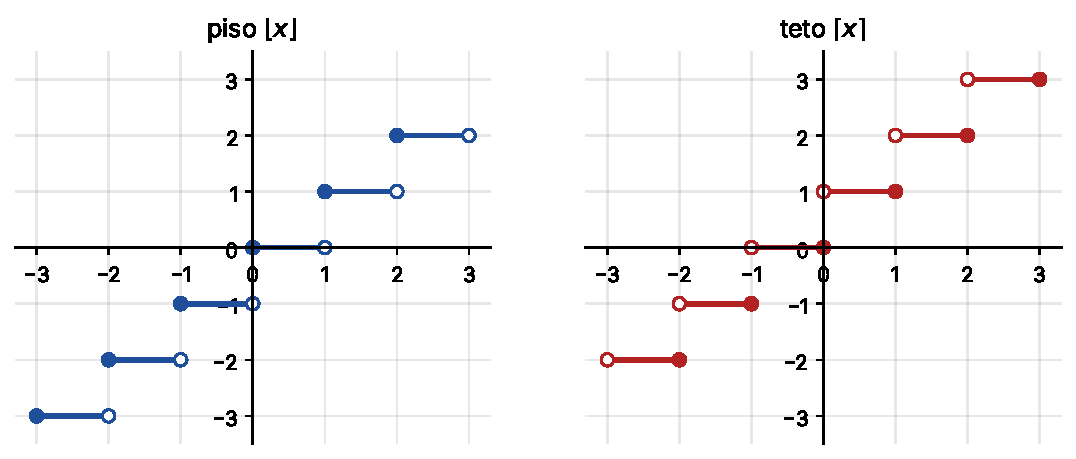
\includegraphics[width=0.85\linewidth]{aula03-piso-teto}
\caption{Gráficos das funções piso e teto. A bolinha cheia indica o valor da função no ponto de salto.}
\end{figure}

\begin{entrada}
for x in [2.1, 2.7, -2.1, -2.7, 3.0]:
    print(f"x = {x:5}  piso = {math.floor(x):3}  teto = {math.ceil(x):3}"
          f"  trunc = {math.trunc(x):3}  round = {round(x):3}")
\end{entrada}
\begin{saida}
x =   2.1  piso =   2  teto =   3  trunc =   2  round =   2
x =   2.7  piso =   2  teto =   3  trunc =   2  round =   3
x =  -2.1  piso =  -3  teto =  -2  trunc =  -2  round =  -2
x =  -2.7  piso =  -3  teto =  -2  trunc =  -2  round =  -3
x =   3.0  piso =   3  teto =   3  trunc =   3  round =   3
\end{saida}

Observe que para números negativos o piso e o \py{trunc} (que apenas descarta a parte decimal, como \py{int()})
são diferentes.

\begin{observacao}
O \py{round} do Python usa o ``arredondamento do banqueiro'': quando o número está exatamente no meio, arredonda
para o \emph{par} mais próximo. Assim \py{round(2.5)} dá \py{2} e \py{round(3.5)} dá \py{4}.
\end{observacao}

\subsection{Raízes, exponenciais e logaritmos}

\begin{entrada}
print(math.sqrt(16), math.sqrt(2), math.cbrt(-8))
print(math.isqrt(50))                 # maior inteiro k com k*k <= 50
print(math.exp(1), math.e)
print(math.log(math.e), math.log(100, 10), math.log10(0.001), math.log2(1024))
\end{entrada}
\begin{saida}
4.0 1.4142135623730951 -2.0
7
2.718281828459045 2.718281828459045
1.0 2.0 -3.0 10.0
\end{saida}

Fora do domínio, as funções do \py{math} geram erro:

% erro
\begin{entrada}
math.sqrt(-4)
\end{entrada}
\begin{saida}
ValueError: math domain error
\end{saida}

Para raízes de números negativos (resultados complexos) existe o módulo \py{cmath}, com as mesmas funções:

\begin{entrada}
import cmath
print(cmath.sqrt(-4), (-4)**0.5)
\end{entrada}
\begin{saida}
2j (1.2246467991473532e-16+2j)
\end{saida}

\paragraph{Exemplo: juros compostos.} Um capital aplicado a uma taxa de 1\% ao mês dobra quando $(1{,}01)^n=2$,
isto é, $n=\dfrac{\ln 2}{\ln 1{,}01}$.

\begin{entrada}
n = math.log(2) / math.log(1.01)
print(f"n = {n:.2f} meses, ou seja, {math.ceil(n)} meses")
\end{entrada}
\begin{saida}
n = 69.66 meses, ou seja, 70 meses
\end{saida}

\subsection{Trigonometria}

As funções trigonométricas usam o ângulo em \textbf{radianos}. Para trabalhar em graus, converta com
\py{math.radians}.

\begin{entrada}
print(math.sin(math.pi/2), math.cos(math.pi))
print(math.sin(30))                     # 30 RADIANOS, não graus!
print(math.sin(math.radians(30)))       # sen(30°)
print(math.degrees(math.atan(1)))       # arctan(1) em graus
print(math.sin(math.pi))                # deveria ser 0...
\end{entrada}
\begin{saida}
1.0 -1.0
-0.9880316240928618
0.49999999999999994
45.0
1.2246467991473532e-16
\end{saida}

O último valor, $1{,}22\times10^{-16}$, é ``zero com erro de arredondamento'': \py{math.pi} é apenas uma
aproximação de $\pi$. Valores muito pequenos como esse devem ser lidos como zero.

\begin{entrada}
print(" graus    sen      cos      tg")
for g in [0, 30, 45, 60]:
    r = math.radians(g)
    print(f"{g:5d} {math.sin(r):8.4f} {math.cos(r):8.4f} {math.tan(r):8.4f}")
\end{entrada}
\begin{saida}
 graus    sen      cos      tg
    0   0.0000   1.0000   0.0000
   30   0.5000   0.8660   0.5774
   45   0.7071   0.7071   1.0000
   60   0.8660   0.5000   1.7321
\end{saida}

\subsection{Funções para inteiros}

\begin{entrada}
print(math.factorial(10), math.factorial(25))
print(math.comb(60, 6))           # jogos possíveis na Mega-Sena
print(math.perm(5, 2))            # arranjos de 5 tomados 2 a 2
print(math.gcd(252, 198), math.lcm(4, 6, 10))
\end{entrada}
\begin{saida}
3628800 15511210043330985984000000
50063860
20
18 60
\end{saida}

% ------------------------------------------------------------
\section{Aplicações em geometria}
% ------------------------------------------------------------

\paragraph{Teorema de Pitágoras.} Em um triângulo retângulo de catetos $a$, $b$ e hipotenusa $c$, vale
$c^2=a^2+b^2$. O exemplo abaixo é o do livro da SBM.

% entradas: 10 | 11
\begin{entrada}
from math import sqrt
a = float(input("Digite o primeiro cateto: "))
b = float(input("Digite o segundo cateto: "))
c = sqrt(a**2 + b**2)          # ou math.hypot(a, b)
print("Hipotenusa:", c)
\end{entrada}
\begin{saida}
Digite o primeiro cateto: 10
Digite o segundo cateto: 11
Hipotenusa: 14.866068747318506
\end{saida}

\paragraph{Lei dos cossenos e fórmula de Herão.} Para um triângulo de lados $a,b,c$, o ângulo $\gamma$ oposto a
$c$ satisfaz $c^2=a^2+b^2-2ab\cos\gamma$, e a área é
$A=\sqrt{s(s-a)(s-b)(s-c)}$, com $s=\frac{a+b+c}{2}$.

\begin{entrada}
def angulos(a, b, c):
    """Ângulos (em graus) opostos aos lados a, b, c."""
    alfa = math.degrees(math.acos((b**2 + c**2 - a**2) / (2*b*c)))
    beta = math.degrees(math.acos((a**2 + c**2 - b**2) / (2*a*c)))
    gama = 180 - alfa - beta
    return alfa, beta, gama

def area_herao(a, b, c):
    s = (a + b + c) / 2
    return math.sqrt(s*(s - a)*(s - b)*(s - c))

print(angulos(3, 4, 5))
print(area_herao(3, 4, 5), area_herao(5, 5, 5))
\end{entrada}
\begin{saida}
(36.86989764584401, 53.13010235415599, 90.0)
6.0 10.825317547305483
\end{saida}

% ------------------------------------------------------------
\section{Atividade: a raiz quadrada pelo método babilônico}
% ------------------------------------------------------------

Como uma calculadora (ou o \py{math.sqrt}) calcula $\sqrt{2}$? Uma ideia muito antiga, atribuída aos
babilônios e descrita por Herão de Alexandria, é a seguinte.

\paragraph{Ideia geométrica.} Queremos um \emph{quadrado} de área $x$; seu lado é $\sqrt{x}$. Começamos com um
\emph{retângulo} de área $x$ e lados $y$ e $x/y$. Se $y$ for menor que $\sqrt x$, então $x/y$ é maior que
$\sqrt x$, e vice-versa: a raiz está sempre entre os dois lados. Tomamos como novo lado a \textbf{média} dos dois,
obtendo um retângulo ``mais quadrado''. Repetindo:
\[
\boxed{\,y_{k+1}=\frac{1}{2}\left(y_k+\frac{x}{y_k}\right)\,},\qquad y_0>0 \text{ qualquer.}
\]

\begin{figure}[ht]
\centering
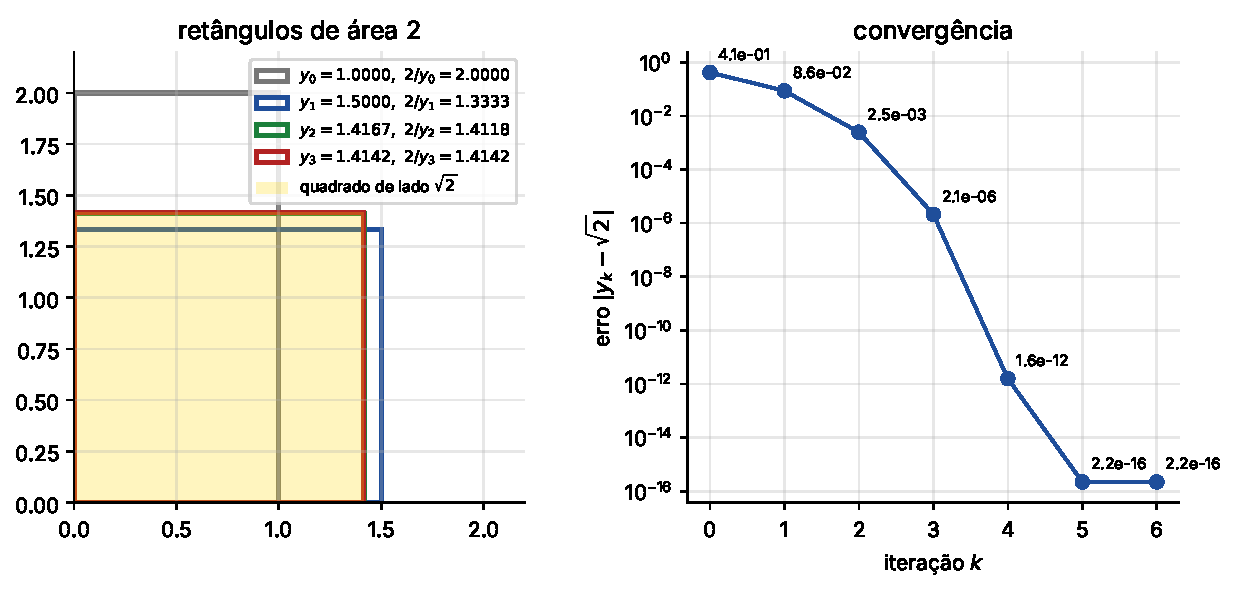
\includegraphics[width=\linewidth]{aula03-babilonico}
\caption{Método babilônico para $\sqrt{2}$, começando com $y_0=1$. À esquerda: os retângulos de área 2 e lados
$y_k$ e $2/y_k$ vão se aproximando de um quadrado. À direita: o erro $|y_k-\sqrt2|$ em escala logarítmica; o número
de casas decimais corretas praticamente dobra a cada passo.}
\label{fig:babilonico}
\end{figure}

\paragraph{Primeira versão.} Seguindo o tutorial do R. Miranda, fazemos um número fixo de repetições:

\begin{entrada}
def minharaizquadrada(x):
    y = 1
    for k in range(1, 10):      # 9 iterações
        y = (y + x/y) / 2
    return y

print(minharaizquadrada(2), math.sqrt(2))
\end{entrada}
\begin{saida}
1.414213562373095 1.4142135623730951
\end{saida}

\paragraph{Acompanhando as iterações.} Vamos imprimir cada aproximação e o seu erro.

\begin{entrada}
x = 2
y = 1.0
for k in range(1, 7):
    y = (y + x/y) / 2
    print(f"k = {k}   y = {y:.16f}   erro = {abs(y - math.sqrt(x)):.2e}")
\end{entrada}
\begin{saida}
k = 1   y = 1.5000000000000000   erro = 8.58e-02
k = 2   y = 1.4166666666666665   erro = 2.45e-03
k = 3   y = 1.4142156862745097   erro = 2.12e-06
k = 4   y = 1.4142135623746899   erro = 1.59e-12
k = 5   y = 1.4142135623730949   erro = 2.22e-16
k = 6   y = 1.4142135623730949   erro = 2.22e-16
\end{saida}

Em apenas 5 passos chegamos ao limite de precisão do \py{float}. Esse método é um caso particular do
\textbf{método de Newton} aplicado a $f(y)=y^2-x$ (que será visto em Cálculo Numérico).

\paragraph{Segunda versão: com critério de parada.} Em vez de um número fixo de passos, paramos quando duas
aproximações consecutivas ficam muito próximas (diferença menor que uma tolerância). Também tratamos os casos
$x<0$ e $x=0$.

\begin{entrada}
def raiz(x, tol=1e-12):
    """Raiz quadrada de x pelo método babilônico."""
    if x < 0:
        print("Erro: x deve ser não negativo")
        return None
    if x == 0:
        return 0.0
    y = x if x > 1 else 1.0          # chute inicial
    passos = 0
    while True:
        novo = (y + x/y) / 2
        passos += 1
        if abs(novo - y) < tol:
            break
        y = novo
    print(f"  ({passos} passos)")
    return novo

for valor in [2, 10, 1e6, 0.0001]:
    r = raiz(valor)
    print(f"raiz({valor}) = {r}   math.sqrt = {math.sqrt(valor)}")
\end{entrada}
\begin{saida}
  (6 passos)
raiz(2) = 1.414213562373095   math.sqrt = 1.4142135623730951
  (7 passos)
raiz(10) = 3.162277660168379   math.sqrt = 3.1622776601683795
  (16 passos)
raiz(1000000.0) = 1000.0   math.sqrt = 1000.0
  (12 passos)
raiz(0.0001) = 0.01   math.sqrt = 0.01
\end{saida}

\begin{desafio}
\begin{enumerate}[label=(\alph*)]
  \item O que acontece se o chute inicial for negativo, por exemplo $y_0=-1$?
  \item Adapte o método para a raiz cúbica, usando $y_{k+1}=\frac{1}{3}\left(2y_k+\frac{x}{y_k^2}\right)$.
  \item (Herão) Calcule $\sqrt{720}$ começando com $y_0=27$ e veja quantos passos são necessários.
\end{enumerate}
\end{desafio}

\begin{professor}
Sugestão: deixar a turma escrever a primeira versão sozinha (10 min) a partir da fórmula no quadro, e só depois
mostrar a tabela de erros. Pergunta para a turma: ``por que o erro para de diminuir em $2{,}22\times10^{-16}$?''
(resposta: é a precisão do \texttt{float}, cerca de 16 algarismos). Para o item (a) do desafio, a sequência
converge para $-\sqrt{x}$.
\end{professor}

% ------------------------------------------------------------
\section{Aplicação: teste de primalidade}
% ------------------------------------------------------------

Na Aula 2 vimos que, para testar se $n$ é primo, basta procurar divisores $d$ com $d\le\sqrt n$. No tutorial do
R. Miranda isso é feito com \py{range(3, int(math.sqrt(n)), 2)}. Vamos testar essa versão:

\begin{entrada}
def checaprimo2(n):
    if n == 2:
        return True
    if n % 2 == 0 or n <= 1:
        return False
    for divisor in range(3, int(math.sqrt(n)), 2):
        if n % divisor == 0:
            return False
    return True

print([n for n in range(2, 60) if checaprimo2(n)])
\end{entrada}
\begin{saida}
[2, 3, 5, 7, 9, 11, 13, 15, 17, 19, 23, 25, 29, 31, 35, 37, 41, 43, 47, 49, 53, 59]
\end{saida}

Há um erro: 9, 15, 25, 35 e 49 aparecem como primos! Como o \py{range} \textbf{não inclui o fim}, o maior
divisor candidato nunca é testado: para $n=15$, \py{int(math.sqrt(15))} vale 3 e \py{range(3, 3, 2)} é vazio;
para $n=49$, o divisor 7 fica de fora. A correção é ir até \py{math.isqrt(n) + 1}:

\begin{entrada}
def eh_primo(n):
    if n == 2:
        return True
    if n % 2 == 0 or n <= 1:
        return False
    for divisor in range(3, math.isqrt(n) + 1, 2):
        if n % divisor == 0:
            return False
    return True

primos = [n for n in range(2, 60) if eh_primo(n)]
print(primos)
print(len([n for n in range(2, 10**5) if eh_primo(n)]), "primos menores que 100000")
\end{entrada}
\begin{saida}
[2, 3, 5, 7, 11, 13, 17, 19, 23, 29, 31, 37, 41, 43, 47, 53, 59]
9592 primos menores que 100000
\end{saida}

\begin{observacao}
O Teorema dos Números Primos diz que a quantidade de primos menores que $N$ é aproximadamente $N/\ln N$. Para
$N=10^5$, \py{1e5 / math.log(1e5)} $\approx 8686$; compare com 9592.
\end{observacao}

% ------------------------------------------------------------
\section{Aplicação: o método da bissecção}
% ------------------------------------------------------------

O Teorema do Valor Intermediário garante: se $f$ é contínua em $[a,b]$ e $f(a)$ e $f(b)$ têm sinais opostos, então
existe $c\in(a,b)$ com $f(c)=0$. O \textbf{método da bissecção} usa isso repetidamente: calcula o ponto médio
$m=\frac{a+b}{2}$ e fica com a metade do intervalo onde a troca de sinal acontece. A cada passo, o
comprimento do intervalo cai pela metade.

\begin{figure}[ht]
\centering
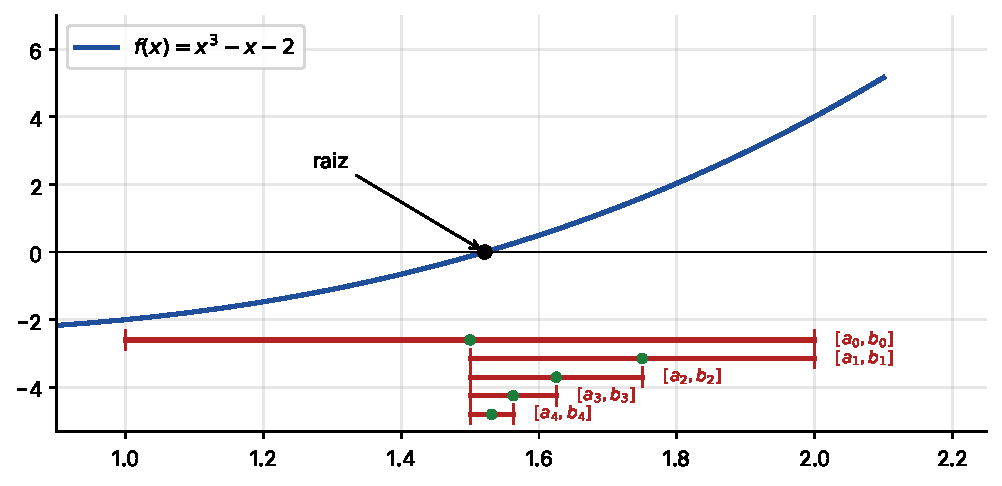
\includegraphics[width=0.9\linewidth]{aula03-bisseccao}
\caption{Bissecção para $f(x)=x^3-x-2$ em $[1,2]$: os intervalos $[a_k,b_k]$ encolhem em torno da raiz.}
\end{figure}

\begin{entrada}
def bisseccao(f, a, b, tol=1e-10):
    if f(a) * f(b) > 0:
        print("f(a) e f(b) têm o mesmo sinal: escolha outro intervalo.")
        return None
    n = 0
    while (b - a) / 2 > tol:
        m = (a + b) / 2
        if f(m) == 0:
            return m
        if f(a) * f(m) < 0:      # a raiz está em [a, m]
            b = m
        else:                    # a raiz está em [m, b]
            a = m
        n += 1
    print(f"  {n} iterações")
    return (a + b) / 2

f = lambda x: x**3 - x - 2
r = bisseccao(f, 1, 2)
print("raiz ~", r, "  f(raiz) =", f(r))

g = lambda x: math.cos(x) - x
print("cos(x) = x  para x ~", bisseccao(g, 0, 1))
\end{entrada}
\begin{saida}
  33 iterações
raiz ~ 1.5213797068572603   f(raiz) = 3.131943593359665e-10
  33 iterações
cos(x) = x  para x ~ 0.7390851332456805
\end{saida}

Como o intervalo é dividido por 2 a cada passo, depois de $n$ passos o erro é no máximo
$\frac{b-a}{2^{n+1}}$. Para garantir erro menor que $10^{-10}$ partindo de $[1,2]$, são necessários
$n\ge \log_2(10^{10})-1\approx 32{,}2$ passos, o que confere com o programa.

% ------------------------------------------------------------
\section{Exercícios}
% ------------------------------------------------------------

\begin{exercicio}[distância e ponto médio]{ex:3-dist}
Escreva uma função \py{distancia(P, Q)} que receba dois pontos do plano como tuplas e devolva a distância entre
eles. Use-a para calcular o perímetro do triângulo de vértices $(0,0)$, $(4,0)$ e $(1,3)$.
\end{exercicio}

\begin{exercicio}[ângulo entre ponteiros]{ex:3-relogio}
Às $h$ horas e $m$ minutos, o ponteiro das horas está a $30h+0{,}5m$ graus da posição das 12h e o dos minutos a
$6m$ graus. Escreva uma função que devolva o menor ângulo entre os ponteiros. Teste com 3h00, 9h45 e 12h30.
\end{exercicio}

\begin{exercicio}[aproximando $e$ e $\pi$]{ex:3-series}
(a) Calcule $\sum_{k=0}^{n}\frac{1}{k!}$ para $n=5,10,15$ e compare com \py{math.e}.
(b) Calcule a série de Leibniz $4\sum_{k=0}^{n}\frac{(-1)^k}{2k+1}$ para $n=10, 1000, 100000$ e compare com
\py{math.pi}. Qual das séries converge mais rápido?
\end{exercicio}

\begin{exercicio}[série de Taylor do seno]{ex:3-seno}
Escreva uma função \py{seno(x, n)} que calcule $\displaystyle\sum_{k=0}^{n}\frac{(-1)^k x^{2k+1}}{(2k+1)!}$ e compare
com \py{math.sin(x)} para $x=1$ e $x=10$, com $n=5$ e $n=20$.
\end{exercicio}

\begin{exercicio}[raiz cúbica]{ex:3-cubica}
Adapte a função \py{raiz} para calcular $\sqrt[3]{x}$ com a iteração $y_{k+1}=\frac{1}{3}\left(2y_k+\frac{x}{y_k^2}\right)$
e compare com \py{math.cbrt}.
\end{exercicio}

\begin{exercicio}[extra: bissecção]{ex:3-bissec}
Use a bissecção para encontrar: (a) a raiz positiva de $x^2-2$ (compare com $\sqrt2$); (b) a solução de
$e^{-x}=x$; (c) a raiz de $x^7+x-1$ em $[0,1]$ (exemplo do tutorial do R. Miranda).
\end{exercicio}

% ============================================================
\chapter{NumPy I: vetores (\emph{arrays}) e cálculo numérico}
\label{cap:aula4}
% ============================================================

\begin{objetivos}
\begin{itemize}
  \item entender a diferença entre uma lista do Python e um \emph{array} do NumPy;
  \item criar \emph{arrays} com \py{np.array}, \py{np.zeros}, \py{np.ones}, \py{np.arange} e \py{np.linspace};
  \item fazer operações elemento a elemento e aplicar funções (\py{np.sin}, \py{np.exp}, ...) a vetores inteiros;
  \item selecionar elementos com índices, fatias e máscaras lógicas;
  \item usar somas, médias, máximos e somas acumuladas; aplicar a regra dos trapézios para integrais.
\end{itemize}
\end{objetivos}

\begin{roteiro}
0--10 min & Por que NumPy? Lista \emph{versus} \emph{array}.\\
10--25 min & Criando \emph{arrays}: \py{array}, \py{zeros}, \py{ones}, \py{arange}, \py{linspace}.\\
25--40 min & Operações elemento a elemento e funções universais; tabela de valores de uma função.\\
40--55 min & Índices, fatias e máscaras; \py{sum}, \py{mean}, \py{max}, \py{argmax}, \py{cumsum}.\\
55--75 min & Aplicações: séries, regra dos trapézios, Monte Carlo.\\
75--90 min & Exercícios.\\
\end{roteiro}

% ------------------------------------------------------------
\section{Por que NumPy?}
% ------------------------------------------------------------

O NumPy (\emph{Numerical Python}) é a biblioteca básica de computação científica em Python. Seu objeto principal é o
\textbf{\emph{array}} (vetor $n$-dimensional): uma sequência de números \emph{do mesmo tipo} com a qual se pode
fazer contas como se fosse um vetor da matemática. Por convenção, importa-se com o apelido \py{np}:

\begin{entrada}
import numpy as np

L = [1, 2, 3, 4]
v = np.array([1, 2, 3, 4])
print(L * 2)          # lista: repete
print(v * 2)          # array: multiplica cada elemento
print(L + [10])       # lista: concatena
print(v + 10)         # array: soma 10 a cada elemento
\end{entrada}
\begin{saida}
[1, 2, 3, 4, 1, 2, 3, 4]
[2 4 6 8]
[1, 2, 3, 4, 10]
[11 12 13 14]
\end{saida}

Repare que o \py{print} de um \emph{array} não tem vírgulas. Além de mais natural para a matemática, o NumPy é
muito mais rápido que as listas para grandes quantidades de números, pois as contas são feitas em código
compilado.

\begin{dica}
Se \py{import numpy} gerar \py{ModuleNotFoundError}, instale com \py{%pip install numpy} em uma célula do Jupyter
e reinicie o kernel.
\end{dica}

% ------------------------------------------------------------
\section{Criando \emph{arrays}}
% ------------------------------------------------------------

\begin{center}
\begin{tabular}{@{}ll@{}}
\toprule
\textbf{Comando} & \textbf{Resultado}\\
\midrule
\py{np.array([1, 2, 3])} & a partir de uma lista\\
\py{np.zeros(n)}, \py{np.ones(n)} & $n$ zeros / $n$ uns (\py{float})\\
\py{np.full(n, c)} & $n$ cópias do valor $c$\\
\py{np.arange(a, b, h)} & $a, a+h, a+2h, \dots$ (menores que $b$), como o \py{range}\\
\py{np.linspace(a, b, n)} & $n$ pontos igualmente espaçados de $a$ até $b$ (\textbf{inclui} $b$)\\
\bottomrule
\end{tabular}
\end{center}

\begin{entrada}
print(np.zeros(3), np.ones(4), np.full(3, 7))
print(np.arange(5))
print(np.arange(2, 9, 2))
print(np.arange(0, 1, 0.25))
print(np.linspace(0, 1, 5))
print(np.linspace(0, 10, num=5))
\end{entrada}
\begin{saida}
[0. 0. 0.] [1. 1. 1. 1.] [7 7 7]
[0 1 2 3 4]
[2 4 6 8]
[0.   0.25 0.5  0.75]
[0.   0.25 0.5  0.75 1.  ]
[ 0.   2.5  5.   7.5 10. ]
\end{saida}

\begin{figure}[ht]
\centering
\begin{tikzpicture}[x=11cm, font=\small]
  \draw[-{Stealth}] (-0.03,0) -- (1.06,0);
  \foreach \t in {0,0.25,0.5,0.75} { \fill[azul] (\t,0) circle (2.6pt); }
  \draw[vermelho, thick] (1,0) circle (3pt);
  \node[anchor=west, font=\ttfamily] at (1.07,0) {arange(0, 1, 0.25)};
  \node[below, font=\scriptsize] at (0,-0.1) {0};  \node[below, font=\scriptsize] at (1,-0.1) {1};
  \node[above, font=\scriptsize, text=azul] at (0.125,0.08) {passo $h=0{,}25$};
  \begin{scope}[yshift=-1.1cm]
  \draw[-{Stealth}] (-0.03,0) -- (1.06,0);
  \foreach \t in {0,0.25,0.5,0.75,1} { \fill[verde] (\t,0) circle (2.6pt); }
  \node[anchor=west, font=\ttfamily] at (1.07,0) {linspace(0, 1, 5)};
  \node[below, font=\scriptsize] at (0,-0.1) {0};  \node[below, font=\scriptsize] at (1,-0.1) {1};
  \node[above, font=\scriptsize, text=verde!70!black] at (0.5,0.08) {5 pontos, extremos incluídos};
  \end{scope}
\end{tikzpicture}
\caption{\texttt{arange} usa o \emph{passo} e exclui o fim; \texttt{linspace} usa a \emph{quantidade de pontos} e inclui o fim.}
\label{fig:arange-linspace}
\end{figure}

\begin{dica}
Para dividir um intervalo $[a,b]$ em pontos (para gráficos, tabelas e integrais), prefira \py{np.linspace}: com
passos decimais o \py{arange} pode incluir ou não o último ponto por causa de arredondamentos.
\end{dica}

Todo \emph{array} tem um tipo (\py{dtype}), uma forma (\py{shape}) e um tamanho (\py{size}):

\begin{entrada}
v = np.array([1, 2, 3])
w = np.array([1, 2.5, 3])
print(v.dtype, w.dtype, v.shape, v.size, v.ndim)
print(np.array([1, 2, 3], dtype=float))
\end{entrada}
\begin{saida}
int64 float64 (3,) 3 1
[1. 2. 3.]
\end{saida}

% ------------------------------------------------------------
\section{Operações elemento a elemento}
% ------------------------------------------------------------

As operações \py{+}, \py{-}, \py{*}, \py{/}, \py{**} entre \emph{arrays} do mesmo tamanho são feitas
\textbf{posição por posição}. Entre um \emph{array} e um número, o número é operado com cada elemento.

\begin{entrada}
u = np.array([1, 2, 3])
v = np.array([4, 5, 6])
print(u + v, u - v, u * v, v / u, u ** 2, 2 ** u)
print(np.dot(u, v), u @ v)       # produto escalar: 1*4 + 2*5 + 3*6
print(np.linalg.norm(u))         # norma: sqrt(1 + 4 + 9)
\end{entrada}
\begin{saida}
[5 7 9] [-3 -3 -3] [ 4 10 18] [4.  2.5 2. ] [1 4 9] [2 4 8]
32 32
3.7416573867739413
\end{saida}

\begin{atencao}
\py{u * v} \textbf{não} é o produto escalar: é o vetor dos produtos $(u_1v_1, u_2v_2, u_3v_3)$. O produto escalar
é \py{np.dot(u, v)} ou \py{u @ v}.
\end{atencao}

\subsection{Funções universais}

O NumPy tem suas próprias versões das funções matemáticas, que funcionam com \emph{arrays} inteiros:
\py{np.sqrt}, \py{np.exp}, \py{np.log}, \py{np.log10}, \py{np.sin}, \py{np.cos}, \py{np.tan},
\py{np.arcsin}, \py{np.arctan}, \py{np.abs}, \py{np.floor}, \py{np.ceil}, além das constantes \py{np.pi} e
\py{np.e}. Isso permite escrever uma função matemática e aplicá-la a muitos pontos de uma vez.

\begin{entrada}
x = np.linspace(0, np.pi, 5)
print(x)
print(np.sin(x))
print(np.round(np.sin(x), 4))
\end{entrada}
\begin{saida}
[0.         0.78539816 1.57079633 2.35619449 3.14159265]
[0.00000000e+00 7.07106781e-01 1.00000000e+00 7.07106781e-01
 1.22464680e-16]
[0.     0.7071 1.     0.7071 0.    ]
\end{saida}

% erro
\begin{entrada}
import math
math.sin(x)
\end{entrada}
\begin{saida}
TypeError: only 0-dimensional arrays can be converted to Python scalars
\end{saida}

As funções do \py{math} só aceitam \emph{um} número; para \emph{arrays}, use as do NumPy.

\paragraph{Tabela de valores.} Definindo uma função com operações do NumPy, ela pode receber um \emph{array}:

\begin{entrada}
def f(x):
    return x**2 * np.exp(-x)

x = np.linspace(0, 4, 9)
y = f(x)
for xi, yi in zip(x, y):
    print(f"{xi:5.2f}  {yi:8.5f}")
\end{entrada}
\begin{saida}
 0.00   0.00000
 0.50   0.15163
 1.00   0.36788
 1.50   0.50204
 2.00   0.54134
 2.50   0.51303
 3.00   0.44808
 3.50   0.36992
 4.00   0.29305
\end{saida}

Esse é exatamente o processo usado para fazer gráficos (Aula 6): calcula-se $f$ em muitos pontos e
ligam-se os pontos.

% ------------------------------------------------------------
\section{Índices, fatias e máscaras}
% ------------------------------------------------------------

Índices e fatias funcionam como nas listas (começando em 0). A novidade são as \textbf{máscaras}: uma condição
aplicada a um \emph{array} produz um \emph{array} de \py{True}/\py{False}, que pode ser usado para selecionar
elementos.

\begin{entrada}
v = np.array([3, -1, 4, -1, 5, -9, 2, 6])
print(v[0], v[-1], v[2:5], v[::2])
print(v > 0)
print(v[v > 0])                 # só os positivos
print(np.sum(v > 0))            # quantos são positivos (True conta 1)
v[v < 0] = 0                    # zera os negativos
print(v)
print(np.where(v > 3, 1, -1))   # 1 onde v > 3, -1 nos outros
\end{entrada}
\begin{saida}
3 6 [ 4 -1  5] [3 4 5 2]
[ True False  True False  True False  True  True]
[3 4 5 2 6]
5
[3 0 4 0 5 0 2 6]
[-1 -1  1 -1  1 -1 -1  1]
\end{saida}

Condições podem ser combinadas com \py{&} (``e'') e \py{|} (``ou''), \textbf{sempre entre parênteses}:

\begin{entrada}
n = np.arange(1, 31)
print(n[(n % 2 == 0) & (n % 3 == 0)])    # múltiplos de 2 e de 3
print(n[(n < 4) | (n > 27)])
\end{entrada}
\begin{saida}
[ 6 12 18 24 30]
[ 1  2  3 28 29 30]
\end{saida}

\begin{atencao}
Com \emph{arrays} não se usa \py{and}/\py{or}, e sim \py{&}/\py{|} com parênteses em cada condição.
\end{atencao}

% ------------------------------------------------------------
\section{Somas, médias e outras reduções}
% ------------------------------------------------------------

\begin{center}
\begin{tabular}{@{}ll@{}}
\toprule
\textbf{Comando} & \textbf{Resultado}\\
\midrule
\py{np.sum(v)}, \py{np.prod(v)} & soma e produto de todos os elementos\\
\py{np.mean(v)}, \py{np.std(v)}, \py{np.median(v)} & média, desvio padrão, mediana\\
\py{np.min(v)}, \py{np.max(v)} & menor e maior valor\\
\py{np.argmin(v)}, \py{np.argmax(v)} & \emph{índice} do menor e do maior valor\\
\py{np.cumsum(v)} & somas acumuladas $v_0,\ v_0+v_1,\ v_0+v_1+v_2, \dots$\\
\py{np.diff(v)} & diferenças $v_1-v_0,\ v_2-v_1,\dots$\\
\py{np.sort(v)} & cópia ordenada\\
\bottomrule
\end{tabular}
\end{center}

Também se pode escrever \py{v.sum()}, \py{v.mean()}, \py{v.max()} etc.

\begin{entrada}
notas = np.array([9.5, 7.5, 10, 8.0, 6.5])
print(notas.mean(), notas.std(), np.median(notas))
print(notas.max(), notas.argmax())
k = np.arange(1, 11)
print(np.cumsum(k))
print(np.diff(k**2))           # diferenças entre quadrados consecutivos
\end{entrada}
\begin{saida}
8.3 1.2884098726725126 8.0
10.0 2
[ 1  3  6 10 15 21 28 36 45 55]
[ 3  5  7  9 11 13 15 17 19]
\end{saida}

\paragraph{Máximo de uma função (aproximado).} Com um \emph{array} de muitos pontos, \py{argmax} dá o ponto onde
$f$ é maior. Para $f(x)=x^2e^{-x}$ em $[0,4]$, o máximo exato ocorre em $x=2$ (Aula 8):

\begin{entrada}
x = np.linspace(0, 4, 4001)
y = f(x)
i = np.argmax(y)
print(f"máximo aproximado em x = {x[i]:.4f}, f(x) = {y[i]:.6f}")
\end{entrada}
\begin{saida}
máximo aproximado em x = 2.0000, f(x) = 0.541341
\end{saida}

% ------------------------------------------------------------
\section{Aplicações}
% ------------------------------------------------------------

\subsection{Somas de séries sem laços}

Com \emph{arrays}, uma soma $\sum_{k=1}^{n} a_k$ se escreve em uma linha, sem \py{for}:

\begin{entrada}
k = np.arange(1, 100001)
print(np.sum(1 / k**2), np.pi**2 / 6)               # série de Basileia
j = np.arange(0, 100000)
print(4 * np.sum((-1)**j / (2*j + 1)), np.pi)        # série de Leibniz
\end{entrada}
\begin{saida}
1.6449240668982266 1.6449340668482264
3.1415826535897926 3.141592653589793
\end{saida}

As somas parciais (para ver a convergência) saem de \py{np.cumsum}:

\begin{entrada}
parciais = np.cumsum(1 / k**2)
for n in [10, 100, 1000, 10000, 100000]:
    print(n, parciais[n-1], np.pi**2/6 - parciais[n-1])
\end{entrada}
\begin{saida}
10 1.5497677311665408 0.09516633568168564
100 1.6349839001848923 0.009950166663334148
1000 1.6439345666815615 0.0009995001666649461
10000 1.6448340718480652 9.999500016122376e-05
100000 1.6449240668982423 9.999949984074163e-06
\end{saida}

O erro se comporta como $1/n$, o que se prova comparando a série com a integral $\int_n^\infty \frac{dx}{x^2}$.

\subsection{Integrais pela regra dos trapézios}

Para aproximar $\int_a^b f(x)\,dx$, dividimos $[a,b]$ em $n$ subintervalos de largura $h=\frac{b-a}{n}$, com pontos
$x_0=a, x_1,\dots,x_n=b$, e somamos as áreas dos trapézios:
\[
\int_a^b f(x)\,dx \approx h\left[\frac{f(x_0)}{2}+f(x_1)+\cdots+f(x_{n-1})+\frac{f(x_n)}{2}\right].
\]

\begin{figure}[ht]
\centering
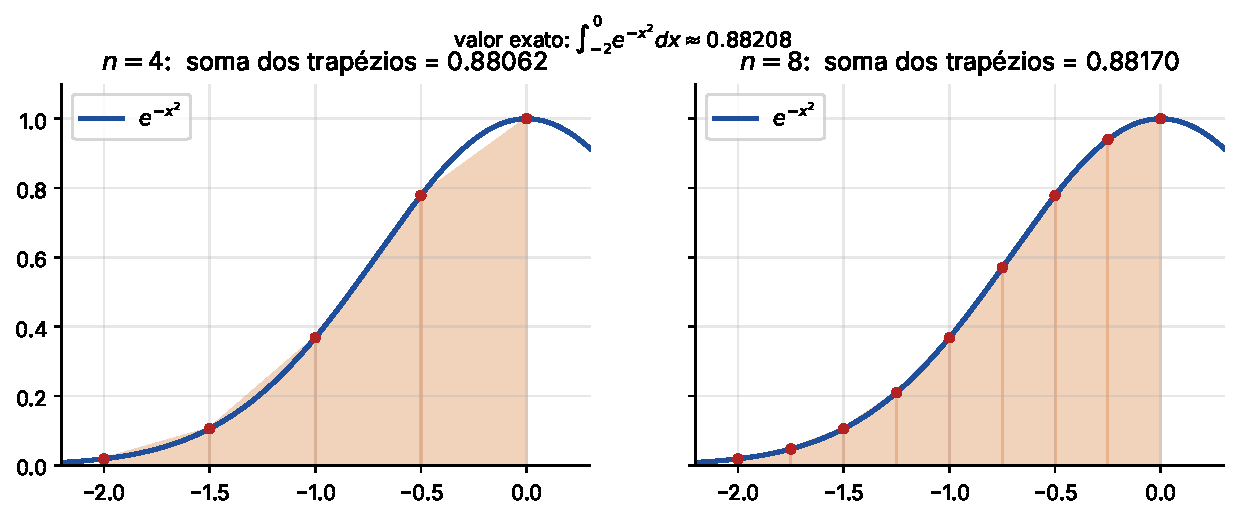
\includegraphics[width=0.95\linewidth]{aula04-trapezios}
\caption{Regra dos trapézios para $f(x)=e^{-x^2}$ em $[-2,0]$ com $n=4$ e $n=8$ subintervalos.}
\end{figure}

Seguindo o livro da SBM, calculamos $\int_{-\infty}^0 e^{-x^2}\,dx=\frac{\sqrt\pi}{2}$, aproximando $-\infty$ por
$-5$ (pois $e^{-25}\approx 10^{-11}$):

\begin{entrada}
def trapezios(f, a, b, n=100):
    x = np.linspace(a, b, n + 1)
    h = x[1] - x[0]
    y = f(x)
    return h * (np.sum(y) - (y[0] + y[-1]) / 2)

g = lambda x: np.exp(-x**2)
exato = np.sqrt(np.pi) / 2
for n in [10, 100, 1000]:
    I = trapezios(g, -5, 0, n)
    print(f"n = {n:5d}   I = {I:.12f}   erro = {abs(I - exato):.2e}")
\end{entrada}
\begin{saida}
n =    10   I = 0.886226925449   erro = 3.51e-12
n =   100   I = 0.886226925451   erro = 1.39e-12
n =  1000   I = 0.886226925451   erro = 1.38e-12
\end{saida}

Já com $n=10$ o resultado é excelente (isso acontece com funções muito ``suaves'' que se anulam nas pontas).
O erro que sobra, da ordem de $10^{-12}$, vem de termos trocado $-\infty$ por $-5$: a área desprezada é
$\int_{-\infty}^{-5}e^{-x^2}dx\approx 1{,}4\times10^{-12}$. Um exemplo mais típico é
$\int_0^1 \frac{4}{1+x^2}\,dx=\pi$:

\begin{entrada}
for n in [10, 20, 40, 80]:
    I = trapezios(lambda x: 4/(1 + x**2), 0, 1, n)
    print(f"n = {n:3d}   I = {I:.10f}   erro = {abs(I - np.pi):.2e}")
\end{entrada}
\begin{saida}
n =  10   I = 3.1399259889   erro = 1.67e-03
n =  20   I = 3.1411759870   erro = 4.17e-04
n =  40   I = 3.1414884869   erro = 1.04e-04
n =  80   I = 3.1415666119   erro = 2.60e-05
\end{saida}

Cada vez que $n$ dobra, o erro cai para $\frac14$: o erro da regra dos trapézios é proporcional a $h^2$.

\begin{observacao}
O NumPy já tem a regra dos trapézios pronta: \py{np.trapezoid(y, x)} (em versões antigas, \py{np.trapz}).
\end{observacao}

\subsection{Números aleatórios: estimando $\pi$ por Monte Carlo}

Sorteando pontos $(x,y)$ uniformemente no quadrado $[0,1]\times[0,1]$, a proporção dos que caem dentro do quarto
de círculo $x^2+y^2\le 1$ se aproxima da razão entre as áreas, $\frac{\pi/4}{1}$.

\begin{figure}[ht]
\centering
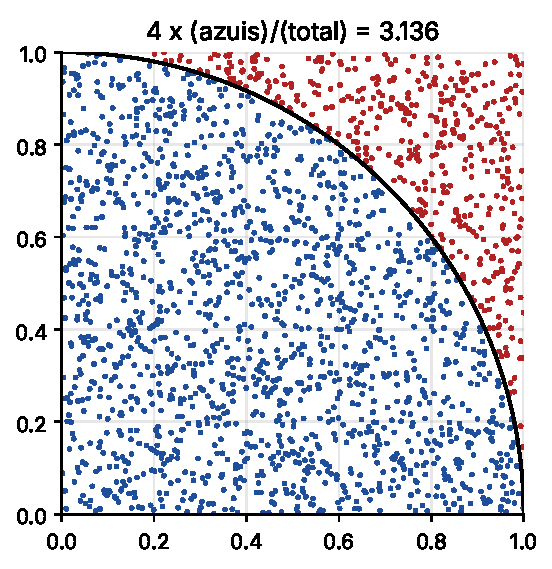
\includegraphics[width=0.42\linewidth]{aula04-montecarlo}
\caption{2000 pontos sorteados: em azul, os que caem dentro do quarto de círculo.}
\end{figure}

\begin{entrada}
rng = np.random.default_rng(2024)      # gerador com "semente" fixa
for n in [100, 10_000, 1_000_000]:
    x = rng.random(n)
    y = rng.random(n)
    dentro = np.sum(x**2 + y**2 <= 1)
    print(f"n = {n:8d}   pi ~ {4 * dentro / n:.5f}")
\end{entrada}
\begin{saida}
n =      100   pi ~ 3.36000
n =    10000   pi ~ 3.13760
n =  1000000   pi ~ 3.14259
\end{saida}

(Com outra semente os valores mudam; o erro típico é da ordem de $1/\sqrt{n}$.)

\subsection{Notação científica}

\begin{entrada}
c = (12 - 3)**100 * 100**100
print(np.format_float_scientific(c, precision=4))
print(f"{float(c):.4e}")
\end{entrada}
\begin{saida}
2.6561e+295
2.6561e+295
\end{saida}

\begin{professor}
O exemplo de Monte Carlo é uma boa oportunidade para discutir o que é uma ``semente'' e por que resultados
aleatórios variam. Se o tempo permitir, peça aos alunos que troquem a semente e comparem os resultados entre si.
\end{professor}

% ------------------------------------------------------------
\section{Exercícios}
% ------------------------------------------------------------

\begin{exercicio}[criando arrays]{ex:4-criar}
Crie, sem usar \py{for}: (a) os 20 primeiros ímpares; (b) 11 pontos igualmente espaçados em $[-1,1]$;
(c) as potências $2^0, 2^1,\dots,2^{10}$; (d) o vetor $\left(1,\frac12,\frac13,\dots,\frac1{10}\right)$.
\end{exercicio}

\begin{exercicio}[tabela]{ex:4-tabela}
Faça uma tabela de $\sin x$, $\cos x$ e $\sin^2x+\cos^2x$ para 7 pontos igualmente espaçados em $[0, \pi]$.
\end{exercicio}

\begin{exercicio}[estatística]{ex:4-estat}
Dadas as alturas (em m) \py{h = np.array([1.72, 1.65, 1.80, 1.58, 1.75, 1.69, 1.83, 1.61])}: calcule a média, o
desvio padrão, quantas pessoas têm mais de 1{,}70\,m e a média apenas dessas pessoas.
\end{exercicio}

\begin{exercicio}[série harmônica]{ex:4-harmonica}
Usando \py{np.cumsum}, encontre o menor $n$ tal que $1+\frac12+\cdots+\frac1n>10$. Compare
$\sum_{k=1}^n\frac1k - \ln n$ para $n=10^6$ com a constante de Euler--Mascheroni $\gamma\approx0{,}5772$.
\end{exercicio}

\begin{exercicio}[regra de Simpson]{ex:4-simpson}
A regra de Simpson (com $n$ par) é
\[\int_a^b f\approx \frac h3\left[f(x_0)+4f(x_1)+2f(x_2)+4f(x_3)+\cdots+4f(x_{n-1})+f(x_n)\right].\]
Implemente-a usando fatias (\py{y[1:-1:2]} e \py{y[2:-1:2]}) e compare com os trapézios em
$\int_0^1\frac{4}{1+x^2}dx$ para $n=10, 20, 40$.
\end{exercicio}

\begin{exercicio}[extra: Monte Carlo para integrais]{ex:4-mc}
Se $x_1,\dots,x_n$ são sorteados uniformemente em $[0,1]$, então $\frac1n\sum f(x_i)\approx\int_0^1 f$. Use isso
para estimar $\int_0^1 e^{-x^2}dx$ e compare com a regra dos trapézios.
\end{exercicio}

% ============================================================
\chapter{NumPy II: matrizes, sistemas lineares e polinômios}
\label{cap:aula5}
% ============================================================

\begin{objetivos}
\begin{itemize}
  \item criar matrizes como \emph{arrays} bidimensionais e acessar linhas, colunas e submatrizes;
  \item distinguir o produto elemento a elemento (\py{*}) do produto de matrizes (\py{@});
  \item calcular transposta, determinante, inversa, posto, autovalores e autovetores com \py{np.linalg};
  \item resolver sistemas lineares com \py{np.linalg.solve} e programar a eliminação de Gauss;
  \item trabalhar com polinômios: raízes, avaliação e ajuste de curvas (\py{np.roots}, \py{np.polyval}, \py{np.polyfit}).
\end{itemize}
\end{objetivos}

\begin{roteiro}
0--15 min & Matrizes no NumPy: criação, \py{shape}, índices, linhas, colunas, matrizes especiais.\\
15--30 min & Operações: soma, \py{*} \emph{versus} \py{@}, transposta, potências.\\
30--45 min & \py{np.linalg}: \py{det}, \py{inv}, \py{solve}, \texttt{matrix\_rank}; sistemas lineares.\\
45--60 min & Eliminação de Gauss programada (exercício do livro da SBM).\\
60--75 min & Autovalores e autovetores; polinômios e ajuste por mínimos quadrados.\\
75--90 min & Exercícios.\\
\end{roteiro}

% ------------------------------------------------------------
\section{Matrizes como \emph{arrays} bidimensionais}
% ------------------------------------------------------------

Uma matriz é criada a partir de uma lista de linhas:

\begin{entrada}
import numpy as np
A = np.array([[1, 2, 3],
              [4, 5, 6]])
print(A)
print("forma:", A.shape, " elementos:", A.size, " dimensões:", A.ndim)
\end{entrada}
\begin{saida}
[[1 2 3]
 [4 5 6]]
forma: (2, 3)  elementos: 6  dimensões: 2
\end{saida}

O elemento da linha $i$ e coluna $j$ é \py{A[i, j]} (contando a partir de 0). O símbolo \py{:} sozinho
significa ``todos'': \py{A[i, :]} é a linha $i$ e \py{A[:, j]} é a coluna $j$.

\begin{figure}[ht]
\centering
\begin{tikzpicture}[font=\ttfamily\small, cel/.style={draw=gray!60, minimum size=0.8cm}]
  \newcommand{\matriz}[3]{%
    \begin{scope}[shift={(#1,0)}]
    \foreach \v [count=\k from 0] in {1,2,3,4,5,6,7,8,9} {
       \pgfmathtruncatemacro{\i}{\k/3} \pgfmathtruncatemacro{\j}{mod(\k,3)}
       \node[cel] at (\j*0.8, -\i*0.8) {\v};
    }
    #2
    \node[font=\ttfamily] at (0.8,-2.7) {#3};
    \end{scope}}
  \matriz{0}{\draw[azul, very thick, fill=azul, fill opacity=0.15] (-0.4,-0.4) rectangle (2.0,-1.2);}{M[1, :]}
  \matriz{3.4}{\draw[verde, very thick, fill=verde, fill opacity=0.15] (1.2,0.4) rectangle (2.0,-2.0);}{M[:, 2]}
  \matriz{6.8}{\draw[vermelho, very thick, fill=vermelho, fill opacity=0.15] (-0.4,0.4) rectangle (1.2,-1.2);}{M[:2, :2]}
  \matriz{10.2}{\draw[laranja, very thick, fill=laranja, fill opacity=0.15] (0.4,-0.4) rectangle (1.2,-1.2);}{M[1, 1]}
\end{tikzpicture}
\caption{Seleção de linha, coluna, submatriz e elemento em \texttt{M = np.arange(1, 10).reshape(3, 3)}.}
\label{fig:fatias-matriz}
\end{figure}

\begin{entrada}
M = np.arange(1, 10).reshape(3, 3)   # 1..9 arrumados em 3 x 3
print(M)
print(M[1, 1], M[0, 2], M[-1, -1])
print(M[1, :], M[:, 2])
print(M[:2, :2])
\end{entrada}
\begin{saida}
[[1 2 3]
 [4 5 6]
 [7 8 9]]
5 3 9
[4 5 6] [3 6 9]
[[1 2]
 [4 5]]
\end{saida}

\begin{maxima}
No Maxima: \texttt{M: matrix([1,2,3],[4,5,6],[7,8,9])}, o elemento é \texttt{M[2,2]} (contando a partir de 1),
a linha é \texttt{row(M,2)} e a coluna \texttt{col(M,3)}. No NumPy a contagem começa em 0: \py{M[1, 1]},
\py{M[1, :]}, \py{M[:, 2]}.
\end{maxima}

\paragraph{Matrizes especiais.}

\begin{entrada}
print(np.eye(3))                  # identidade
print(np.zeros((2, 3)))           # nula 2 x 3 (note os parênteses duplos)
print(np.diag([1, 2, 3]))         # diagonal
print(np.ones((2, 2), dtype=int))
\end{entrada}
\begin{saida}
[[1. 0. 0.]
 [0. 1. 0.]
 [0. 0. 1.]]
[[0. 0. 0.]
 [0. 0. 0.]]
[[1 0 0]
 [0 2 0]
 [0 0 3]]
[[1 1]
 [1 1]]
\end{saida}

Também podemos construir uma matriz a partir de uma fórmula para $a_{ij}$. Por exemplo, a matriz de Hilbert
$h_{ij}=\frac{1}{i+j-1}$ (com $i,j$ começando em 1):

\begin{entrada}
n = 4
i = np.arange(1, n + 1).reshape(n, 1)    # coluna
j = np.arange(1, n + 1).reshape(1, n)    # linha
H = 1 / (i + j - 1)                      # "broadcasting": vira n x n
print(np.round(H, 4))
\end{entrada}
\begin{saida}
[[1.     0.5    0.3333 0.25  ]
 [0.5    0.3333 0.25   0.2   ]
 [0.3333 0.25   0.2    0.1667]
 [0.25   0.2    0.1667 0.1429]]
\end{saida}

% ------------------------------------------------------------
\section{Operações com matrizes}
% ------------------------------------------------------------

\begin{center}
\begin{tabular}{@{}lll@{}}
\toprule
\textbf{Matemática} & \textbf{NumPy} & \textbf{Observação}\\
\midrule
$A+B$, $A-B$, $kA$ & \py{A + B}, \py{A - B}, \py{k * A} & \\
$AB$ (produto de matrizes) & \py{A @ B} ou \py{np.dot(A, B)} & \textbf{não} é \py{A * B}\\
$A^T$ & \py{A.T} ou \py{np.transpose(A)} & \\
$A^n$ & \py{np.linalg.matrix_power(A, n)} & \textbf{não} é \py{A**n}\\
$\det A$ & \py{np.linalg.det(A)} & resultado aproximado\\
$A^{-1}$ & \py{np.linalg.inv(A)} & \\
$\operatorname{posto}(A)$ & \py{np.linalg.matrix_rank(A)} & \\
$\operatorname{tr}(A)$ & \py{np.trace(A)} & \\
solução de $Ax=b$ & \py{np.linalg.solve(A, b)} & $A$ quadrada e invertível\\
autovalores/autovetores & \py{np.linalg.eig(A)} & \\
\bottomrule
\end{tabular}
\end{center}

\begin{entrada}
A = np.array([[1, 2], [-3, 1]])
B = np.array([[2, 5], [4, 10]])
print("A * B =\n", A * B)      # elemento a elemento
print("A @ B =\n", A @ B)      # produto de matrizes
print("B @ A =\n", B @ A)      # em geral AB != BA
print("A^T =\n", A.T)
\end{entrada}
\begin{saida}
A * B =
 [[  2  10]
 [-12  10]]
A @ B =
 [[10 25]
 [-2 -5]]
B @ A =
 [[-13   9]
 [-26  18]]
A^T =
 [[ 1 -3]
 [ 2  1]]
\end{saida}

\begin{atencao}
\py{A * B} e \py{A ** 2} operam \textbf{elemento a elemento}. Para o produto matricial use \py{A @ B}; para
potências, \py{A @ A} ou \py{np.linalg.matrix_power(A, n)}. Multiplicar matrizes de tamanhos incompatíveis
gera \py{ValueError}.
\end{atencao}

\begin{entrada}
print(np.linalg.det(A), np.linalg.det(B))
Ainv = np.linalg.inv(A)
print(Ainv)
print(A @ Ainv)
print(np.allclose(A @ Ainv, np.eye(2)))
\end{entrada}
\begin{saida}
7.000000000000001 0.0
[[ 0.14285714 -0.28571429]
 [ 0.42857143  0.14285714]]
[[1. 0.]
 [0. 1.]]
True
\end{saida}

Note o pequeno erro de arredondamento: $\det A=7$, mas apareceu \py{7.000000000000001}. Erros desse tipo
(da ordem de $10^{-16}$) podem aparecer em qualquer conta com \py{float}; por isso, para comparar matrizes,
usa-se \py{np.allclose}, que admite uma pequena tolerância. Os cálculos \emph{exatos} (como no Maxima) serão feitos com o SymPy na Aula 10.

% erro
\begin{entrada}
np.linalg.inv(B)            # det(B) = 0
\end{entrada}
\begin{saida}
LinAlgError: Singular matrix
\end{saida}

\paragraph{Exemplo: Fibonacci por potências de matriz.} Como
$\begin{pmatrix}F_{n+1}\\F_n\end{pmatrix}=\begin{pmatrix}1&1\\1&0\end{pmatrix}\begin{pmatrix}F_{n}\\F_{n-1}\end{pmatrix}$,
temos $\begin{pmatrix}1&1\\1&0\end{pmatrix}^n=\begin{pmatrix}F_{n+1}&F_n\\F_n&F_{n-1}\end{pmatrix}$.

\begin{entrada}
Q = np.array([[1, 1], [1, 0]])
print(np.linalg.matrix_power(Q, 10))
\end{entrada}
\begin{saida}
[[89 55]
 [55 34]]
\end{saida}

% ------------------------------------------------------------
\section{Sistemas lineares}
% ------------------------------------------------------------

O sistema
\[
\begin{cases} x_0+2x_1=1\\ 3x_0+5x_1=2\end{cases}
\qquad\Longleftrightarrow\qquad
\underbrace{\begin{pmatrix}1&2\\3&5\end{pmatrix}}_{A}\begin{pmatrix}x_0\\x_1\end{pmatrix}=\underbrace{\begin{pmatrix}1\\2\end{pmatrix}}_{b}
\]
(exemplo do livro da SBM) se resolve com \py{np.linalg.solve(A, b)}. Geometricamente, a solução é o ponto de
encontro das duas retas (Figura~\ref{fig:retas}).

\begin{figure}[ht]
\centering
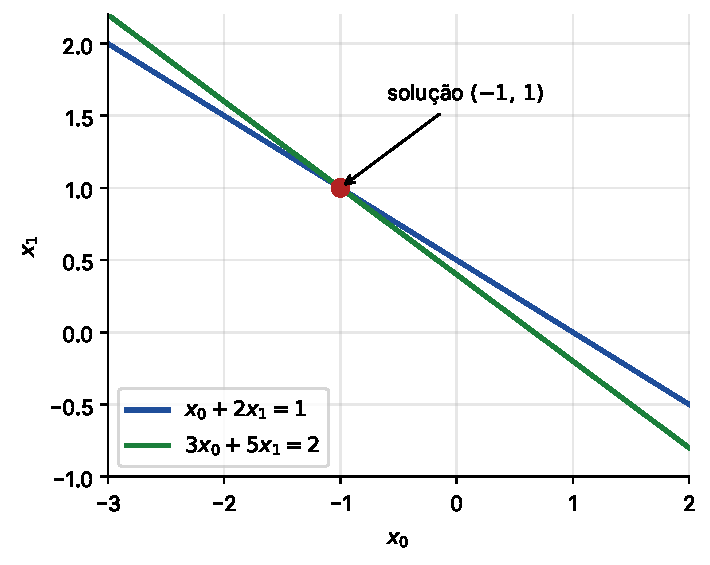
\includegraphics[width=0.55\linewidth]{aula05-retas}
\caption{As retas $x_0+2x_1=1$ e $3x_0+5x_1=2$ se encontram em $(-1,1)$.}
\label{fig:retas}
\end{figure}

\begin{entrada}
A = np.array([[1, 2], [3, 5]])
b = np.array([1, 2])
x = np.linalg.solve(A, b)
print(x)
print(np.allclose(A @ x, b))        # verificação: Ax = b ?
\end{entrada}
\begin{saida}
[-1.  1.]
True
\end{saida}

Um sistema $3\times3$:
\[
\begin{cases} x+y-2z=1\\ x+y-z=3\\ 3x+y-z=3 \end{cases}
\]

\begin{entrada}
A = np.array([[1, 1, -2], [1, 1, -1], [3, 1, -1]])
b = np.array([1, 3, 3])
print(np.linalg.det(A))
print(np.linalg.solve(A, b))
\end{entrada}
\begin{saida}
2.0000000000000004
[0. 5. 2.]
\end{saida}

\begin{observacao}
\py{np.linalg.solve} só funciona para matrizes quadradas invertíveis. Se o sistema for impossível ou
indeterminado ($\det A=0$), ele gera \py{LinAlgError}. Para analisar esses casos, compare o posto da matriz dos
coeficientes com o da matriz ampliada (Teorema de Rouché--Capelli), usando \py{np.linalg.matrix_rank}, ou use o
SymPy (Aula 10).
\end{observacao}

\begin{entrada}
A = np.array([[1, 2], [2, 4]])
for b in [np.array([3, 6]), np.array([3, 7])]:
    Ab = np.column_stack([A, b])            # matriz ampliada [A | b]
    print(b, np.linalg.matrix_rank(A), np.linalg.matrix_rank(Ab))
\end{entrada}
\begin{saida}
[3 6] 1 1
[3 7] 1 2
\end{saida}

No primeiro caso os postos são iguais (1) e menores que o número de incógnitas: sistema possível e
indeterminado. No segundo, os postos diferem: sistema impossível.

% ------------------------------------------------------------
\section{Programando a eliminação de Gauss}
% ------------------------------------------------------------

O livro da SBM (Exemplo 3.35 e Exercício 3) propõe programar o método de eliminação de Gauss. Com o NumPy as
operações com linhas ficam bem mais simples, pois \py{M[i]} é a linha $i$ inteira e podemos fazer
\py{M[j] = M[j] - fator * M[i]}.

O método tem duas etapas:
\begin{enumerate}
  \item \textbf{Escalonamento}: para cada coluna $i$, escolhe-se como pivô o elemento de maior módulo na coluna
  (da linha $i$ para baixo), troca-se a sua linha com a linha $i$, e zeram-se os elementos abaixo do pivô com
  $L_j \leftarrow L_j - \frac{a_{ji}}{a_{ii}}L_i$.
  \item \textbf{Retrossubstituição}: no sistema triangular $Ux=c$, calcula-se $x_{n-1}$, depois $x_{n-2}$, e assim
  por diante: $x_i=\dfrac{c_i-\sum_{j>i}u_{ij}x_j}{u_{ii}}$.
\end{enumerate}

\begin{entrada}
def escalona(A, b):
    """Escalona a matriz ampliada [A | b] (com pivoteamento parcial)."""
    M = np.column_stack([A, b]).astype(float)
    n = len(b)
    for i in range(n - 1):
        p = i + np.argmax(np.abs(M[i:, i]))   # linha do maior pivô
        if M[p, i] == 0:
            raise ValueError("matriz singular")
        M[[i, p]] = M[[p, i]]                 # troca as linhas i e p
        for j in range(i + 1, n):
            fator = M[j, i] / M[i, i]
            M[j] = M[j] - fator * M[i]
    return M

def retrossubstituicao(M):
    n = M.shape[0]
    x = np.zeros(n)
    for i in range(n - 1, -1, -1):            # i = n-1, ..., 1, 0
        x[i] = (M[i, -1] - M[i, i+1:n] @ x[i+1:]) / M[i, i]
    return x

def gauss(A, b):
    return retrossubstituicao(escalona(A, b))
\end{entrada}

Vamos testar com o sistema do livro da SBM, cuja matriz ampliada é
\[
\left(\begin{array}{rrrr|r}
1 & -1 & 2 & -1 & -8\\
2 & -2 & 3 & -3 & -20\\
1 & 1 & 1 & 0 & -2\\
1 & -1 & 4 & -3 & 4
\end{array}\right).
\]
Repare que, depois do primeiro passo, aparece um zero na posição do segundo pivô: sem a troca de linhas o método
falharia.

\begin{entrada}
A = np.array([[1, -1, 2, -1], [2, -2, 3, -3], [1, 1, 1, 0], [1, -1, 4, -3]])
b = np.array([-8, -20, -2, 4])
np.set_printoptions(precision=3, suppress=True)
print(escalona(A, b))
x = gauss(A, b)
print("x =", x)
print("conferindo com solve:", np.linalg.solve(A, b))
\end{entrada}
\begin{saida}
[[  2.   -2.    3.   -3.  -20. ]
 [  0.    2.   -0.5   1.5   8. ]
 [  0.    0.    2.5  -1.5  14. ]
 [  0.    0.    0.    0.8  -0.8]]
x = [-13.   6.   5.  -1.]
conferindo com solve: [-13.   6.   5.  -1.]
\end{saida}

\begin{observacao}
O comando \py{np.set_printoptions(precision=3, suppress=True)} faz o NumPy mostrar 3 casas decimais e não usar
notação científica para números muito pequenos. Ele vale para o resto do notebook; para voltar ao padrão, use
\py{np.set_printoptions(precision=8, suppress=False)}.
\end{observacao}

% ------------------------------------------------------------
\section{Autovalores e autovetores}
% ------------------------------------------------------------

Um número $\lambda$ é autovalor de $A$ se existe $v\neq0$ com $Av=\lambda v$. O comando \py{np.linalg.eig(A)}
devolve os autovalores e uma matriz cujas \textbf{colunas} são autovetores (normalizados, com norma 1). Para
matrizes \textbf{simétricas} há o \py{np.linalg.eigh}, que devolve os autovalores reais e em ordem crescente.

\begin{entrada}
A = np.array([[2, 1], [1, 2]])
autovalores, V = np.linalg.eigh(A)     # A é simétrica
print(autovalores)
print(V)
v = V[:, 1]                          # autovetor da coluna 1 (lambda = 3)
print(A @ v, autovalores[1] * v)     # A v = lambda v
\end{entrada}
\begin{saida}
[1. 3.]
[[-0.707  0.707]
 [ 0.707  0.707]]
[2.121 2.121] [2.121 2.121]
\end{saida}

\begin{figure}[ht]
\centering
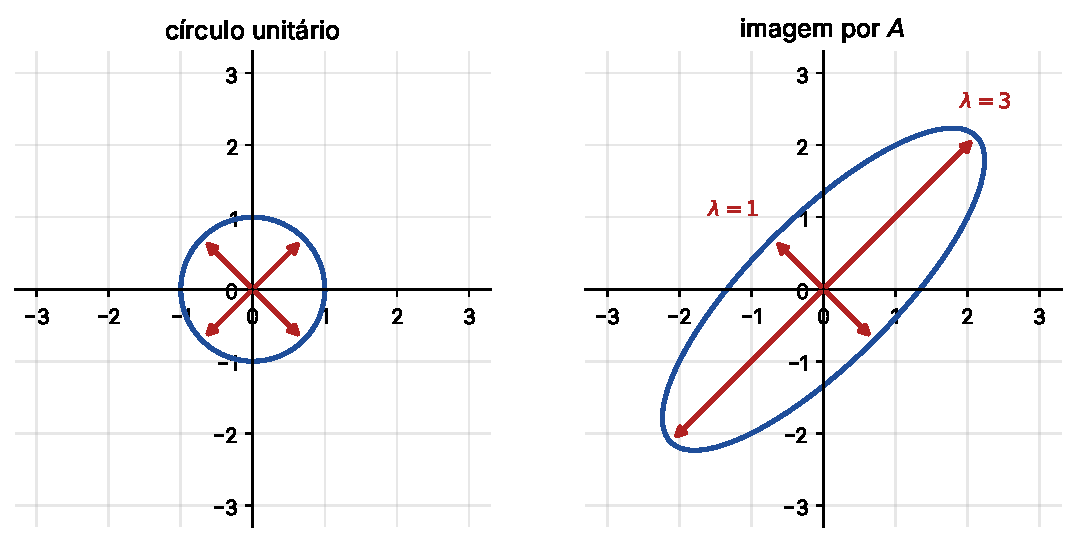
\includegraphics[width=0.8\linewidth]{aula05-transformacao}
\caption{A matriz $A=\begin{pmatrix}2&1\\1&2\end{pmatrix}$ transforma o círculo unitário em uma elipse. Os
autovetores (em vermelho) são as direções que não giram: são apenas esticadas, pelos fatores $\lambda=3$ e $\lambda=1$.}
\end{figure}

Para uma matriz de rotação de $90^\circ$ nenhuma direção é preservada, e os autovalores são complexos:

\begin{entrada}
R = np.array([[0, -1], [1, 0]])
print(np.linalg.eig(R)[0])
\end{entrada}
\begin{saida}
[0.+1.j 0.-1.j]
\end{saida}

% ------------------------------------------------------------
\section{Polinômios}
% ------------------------------------------------------------

No NumPy, um polinômio é representado pela lista de coeficientes, \textbf{do maior grau para o menor}:
$p(x)=x^3-6x^2+11x-6$ é \py{[1, -6, 11, -6]}.

\begin{entrada}
p = [1, -6, 11, -6]
print(np.roots(p))                    # raízes
print(np.polyval(p, [0, 1, 4]))       # p(0), p(1), p(4)
print(np.roots([1, 0, 1]))            # x^2 + 1: raízes complexas
print(np.poly([1, 2, 3]))             # polinômio com raízes 1, 2, 3
\end{entrada}
\begin{saida}
[3. 2. 1.]
[-6  0  6]
[-0.+1.j  0.-1.j]
[ 1. -6. 11. -6.]
\end{saida}

\paragraph{Ajuste de curvas (mínimos quadrados).} Dados pontos $(x_i,y_i)$ experimentais, \py{np.polyfit(x, y, grau)}
encontra o polinômio do grau pedido que melhor se ajusta aos dados (minimizando $\sum (p(x_i)-y_i)^2$).

\begin{entrada}
x = np.array([0, 1, 2, 3, 4, 5])
y = np.array([1.1, 2.9, 5.2, 7.1, 8.8, 11.2])
a, b = np.polyfit(x, y, 1)            # reta y = a x + b
print(f"y = {a:.3f} x + {b:.3f}")
print(f"previsão para x = 6: {np.polyval([a, b], 6):.2f}")
\end{entrada}
\begin{saida}
y = 2.003 x + 1.043
previsão para x = 6: 13.06
\end{saida}

O gráfico desses dados com a reta ajustada é feito na Aula~6.

\begin{professor}
Se a turma já viu escalonamento em Álgebra Linear, vale fazer o primeiro passo da eliminação no quadro e comparar
com a saída de \texttt{escalona}. A função usa \texttt{M[[i, p]] = M[[p, i]]} para trocar linhas, um recurso
(``indexação por lista'') que pode precisar de explicação.
\end{professor}

% ------------------------------------------------------------
\section{Exercícios}
% ------------------------------------------------------------

\begin{exercicio}[operações]{ex:5-ops}
Sejam $A=\begin{pmatrix}1&2&0\\0&1&3\\4&0&1\end{pmatrix}$ e $B=\begin{pmatrix}2&0&1\\1&1&0\\0&3&1\end{pmatrix}$.
Calcule $A+B$, $AB$, $BA$, $A^TB$, $\det(AB)$ e $\det A\cdot\det B$. Verifique que $(AB)^T=B^TA^T$.
\end{exercicio}

\begin{exercicio}[sistema]{ex:5-sistema}
Resolva com \py{np.linalg.solve} e com a função \py{gauss}:
$\begin{cases}2x+y-z=8\\-3x-y+2z=-11\\-2x+y+2z=-3\end{cases}$.
\end{exercicio}

\begin{exercicio}[matriz de Hilbert]{ex:5-hilbert}
Para $n=4, 8, 12$, crie a matriz de Hilbert $H_n$, tome $x=(1,1,\dots,1)$, calcule $b=H_nx$ e resolva $H_ny=b$.
Compare $y$ com $x$. O que acontece? (Pesquise ``matriz mal condicionada'' e use \py{np.linalg.cond}.)
\end{exercicio}

\begin{exercicio}[autovalores]{ex:5-autov}
Calcule os autovalores e autovetores de $\begin{pmatrix}4&1\\2&3\end{pmatrix}$ e verifique $Av=\lambda v$ para cada par.
Confira que a soma dos autovalores é o traço e o produto é o determinante.
\end{exercicio}

\begin{exercicio}[polinômios]{ex:5-poli}
Encontre as raízes de $x^4-5x^2+4$ e de $x^3-2x-5$. Use \py{np.polyval} para conferir que são raízes.
\end{exercicio}

\begin{exercicio}[extra: ajuste de parábola]{ex:5-ajuste}
Um objeto é lançado e sua altura (m) é medida nos instantes $t=0, 0{,}5, 1, 1{,}5, 2, 2{,}5$\,s:
$h=1{,}0;\ 7{,}9;\ 12{,}4;\ 14{,}6;\ 14{,}3;\ 11{,}7$. Ajuste uma parábola $h(t)=at^2+bt+c$ e estime a aceleração da
gravidade ($g\approx-2a$) e o instante de altura máxima.
\end{exercicio}

% ============================================================
\chapter{Gráficos com Matplotlib}
\label{cap:aula6}
% ============================================================

\begin{objetivos}
\begin{itemize}
  \item entender como o computador desenha o gráfico de uma função (pontos ligados por segmentos);
  \item fazer gráficos com \py{plt.plot} e personalizar cores, estilos, legendas, títulos e eixos;
  \item colocar vários gráficos em uma mesma figura (\py{plt.subplots});
  \item desenhar curvas paramétricas, curvas em coordenadas polares e curvas de nível;
  \item desenhar superfícies e curvas no espaço; salvar figuras em arquivo.
\end{itemize}
\end{objetivos}

\begin{roteiro}
0--15 min & Primeiro gráfico; discretização com \py{linspace}; poucos \emph{versus} muitos pontos.\\
15--30 min & Personalização: cores, estilos, legenda, título, eixos, grade; vários gráficos.\\
30--40 min & \py{subplots}; gráficos de dados (\py{scatter}) e reta ajustada.\\
40--55 min & Curvas paramétricas e polares; descontinuidades.\\
55--70 min & \py{meshgrid}, curvas de nível e curvas implícitas.\\
70--85 min & Superfícies e curvas em 3D. Salvando figuras.\\
85--90 min & Exercícios para casa.\\
\end{roteiro}

% ------------------------------------------------------------
\section{O primeiro gráfico}
% ------------------------------------------------------------

O Matplotlib é a biblioteca de gráficos mais usada em Python. Usamos seu submódulo \py{pyplot}, importado com o
apelido \py{plt}, junto com o NumPy:

\begin{codigo}
import numpy as np
import matplotlib.pyplot as plt
\end{codigo}

Para o computador, o gráfico de $y=f(x)$ é um conjunto de pontos $(x_i, f(x_i))$ ligados por segmentos de reta.
Os passos são sempre os mesmos:
\begin{enumerate}
  \item \textbf{discretizar} o intervalo: \py{x = np.linspace(a, b, n)};
  \item calcular \py{y = f(x)} (com funções do NumPy);
  \item desenhar com \py{plt.plot(x, y)} e mostrar com \py{plt.show()}.
\end{enumerate}

% figura: aula06-primeiro
\begin{entrada}
import numpy as np
import matplotlib.pyplot as plt

x = np.linspace(-3, 3, 50)     # 50 pontos entre -3 e 3
y = x**2 + 1
plt.plot(x, y)
plt.show()
\end{entrada}
\saidafig[0.5]{aula06-primeiro}

Com poucos pontos, o ``gráfico'' vira uma poligonal. É por isso que um esboço com 4 pontos não é um bom gráfico:

% figura: aula06-poucos
\begin{entrada}
x = np.linspace(-3, 3, 4)
plt.plot(x, x**2 + 1, "o-")    # "o-": bolinhas ligadas por linhas
plt.show()
\end{entrada}
\saidafig[0.5]{aula06-poucos}

\begin{dica}
No JupyterLab o gráfico aparece logo abaixo da célula. O \py{plt.show()} no fim evita que apareçam linhas de
texto como \py{[<matplotlib.lines.Line2D at 0x...>]} antes da figura.
\end{dica}

% ------------------------------------------------------------
\section{Personalizando o gráfico}
% ------------------------------------------------------------

O terceiro argumento de \py{plt.plot} é uma \emph{string de formato} que combina cor, marcador e tipo de linha:

\begin{center}
\begin{tabular}{@{}llllll@{}}
\toprule
\multicolumn{2}{c}{\textbf{Cores}} & \multicolumn{2}{c}{\textbf{Linhas}} & \multicolumn{2}{c}{\textbf{Marcadores}}\\
\cmidrule(r){1-2}\cmidrule(lr){3-4}\cmidrule(l){5-6}
\py{"b"} & azul & \py{"-"} & contínua & \py{"o"} & círculo\\
\py{"r"} & vermelho & \py{"--"} & tracejada & \py{"s"} & quadrado\\
\py{"g"} & verde & \py{":"} & pontilhada & \py{"^"} & triângulo\\
\py{"k"} & preto & \py{"-."} & traço-ponto & \py{"*"} & estrela\\
\py{"m"}, \py{"c"}, \py{"y"} & magenta, ciano, amarelo & & & \py{"."} & ponto\\
\bottomrule
\end{tabular}
\end{center}

Exemplos: \py{"r--"} (vermelho tracejado), \py{"bo"} (só bolinhas azuis), \py{"k-o"} (linha preta com bolinhas).
Também se pode usar os parâmetros \py{color="purple"}, \py{linestyle="--"}, \py{linewidth=2}, \py{marker="o"}.

\begin{center}
\begin{tabular}{@{}ll@{}}
\toprule
\textbf{Comando} & \textbf{Efeito}\\
\midrule
\py{plt.plot(x, y, label="f")}, \py{plt.legend()} & legenda\\
\py{plt.title("...")}, \py{plt.xlabel("x")}, \py{plt.ylabel("y")} & título e eixos\\
\py{plt.xlim(a, b)}, \py{plt.ylim(c, d)} & janela de visualização\\
\py{plt.grid(True)} & grade\\
\py{plt.axhline(0)}, \py{plt.axvline(0)} & retas $y=0$ e $x=0$\\
\py{plt.axis("equal")} & mesma escala nos dois eixos\\
\py{plt.figure(figsize=(8, 4))} & tamanho da figura (em polegadas)\\
\bottomrule
\end{tabular}
\end{center}

Textos entre \verb|$...$| são escritos como fórmulas do \LaTeX: \py{label=r"$\sin(x)$"} (o \py{r} antes das aspas
evita problemas com a barra invertida).

% figura: aula06-personalizado
\begin{entrada}
x = np.linspace(-2*np.pi, 2*np.pi, 400)
plt.figure(figsize=(8, 4))
plt.plot(x, np.sin(x), "b-", label=r"$\sin x$")
plt.plot(x, np.cos(x), "r--", label=r"$\cos x$")
plt.plot(x, np.sin(x)**2, color="green", linewidth=2.5, label=r"$\sin^2 x$")
plt.axhline(0, color="black", linewidth=0.8)
plt.axvline(0, color="black", linewidth=0.8)
plt.title("Funções trigonométricas")
plt.xlabel("x")
plt.ylabel("y")
plt.ylim(-1.5, 1.5)
plt.grid(True)
plt.legend()
plt.show()
\end{entrada}
\saidafig[0.85]{aula06-personalizado}

\paragraph{Dados \emph{versus} posição.} Se \py{plt.plot} receber apenas um \emph{array}, os valores são colocados
no eixo $y$ e o eixo $x$ é a posição $0,1,2,\dots$ (exemplo do livro da SBM):

% figura: aula06-sbm
\begin{entrada}
a = np.array([2, 1, 5, 7, 4, 6, 8, 14, 10, 9, 18, 20, 22])
b = np.sort(a)
plt.plot(a, "o-", label="dados")
plt.plot(b, color="red", label="dados ordenados")
plt.legend()
plt.show()
\end{entrada}
\saidafig[0.5]{aula06-sbm}

\begin{maxima}
No Maxima: \texttt{plot2d([sin(x), cos(x)], [x, -2*\%pi, 2*\%pi], [y, -1.5, 1.5])}. No Matplotlib não se passa a
\emph{fórmula}, e sim os \emph{pontos}; por isso é preciso criar o \py{x} com \py{linspace}. Na Aula 7 veremos o
\py{sp.plot} do SymPy, que funciona como o \texttt{plot2d}.
\end{maxima}

% ------------------------------------------------------------
\section{Vários gráficos em uma figura}
% ------------------------------------------------------------

Para colocar gráficos lado a lado, usamos \py{fig, ax = plt.subplots(linhas, colunas)}. A variável \py{ax} passa
a ser uma tabela de ``eixos'', e cada gráfico é desenhado com \py{ax[i, j].plot(...)}. Com os eixos os comandos de
personalização têm o prefixo \py{set_}: \py{ax.set_title}, \py{ax.set_xlabel}, \py{ax.set_ylim}...

% figura: aula06-subplots
\begin{entrada}
x = np.linspace(-2, 2, 200)
fig, ax = plt.subplots(2, 2, figsize=(8, 6))
ax[0, 0].plot(x, x**3 - x)
ax[0, 0].set_title(r"$x^3 - x$")
ax[0, 1].plot(x, np.exp(x), "r")
ax[0, 1].set_title(r"$e^x$")
ax[1, 0].plot(x, np.abs(x), "g")
ax[1, 0].set_title(r"$|x|$")
ax[1, 1].plot(x, np.floor(x), "m.")
ax[1, 1].set_title(r"$\lfloor x \rfloor$")
for eixo in ax.flat:          # aplica a todos os quatro
    eixo.grid(True)
plt.tight_layout()            # evita sobreposição dos títulos
plt.show()
\end{entrada}
\saidafig[0.75]{aula06-subplots}

\paragraph{Famílias de curvas.} Um \py{for} desenha várias curvas de uma vez, por exemplo $y=x^n$ para vários $n$:

% figura: aula06-familia
\begin{entrada}
x = np.linspace(0, 1.5, 200)
for n in [1, 2, 3, 4]:
    plt.plot(x, x**n, label=f"$x^{n}$")
plt.ylim(0, 3)
plt.legend()
plt.grid(True)
plt.show()
\end{entrada}
\saidafig[0.5]{aula06-familia}

\paragraph{Dados experimentais e reta ajustada.} Pontos isolados são desenhados com \py{plt.scatter} (ou com
\py{"o"}). Retomando os dados da Aula 5:

% figura: aula06-ajuste
\begin{entrada}
xd = np.array([0, 1, 2, 3, 4, 5])
yd = np.array([1.1, 2.9, 5.2, 7.1, 8.8, 11.2])
a, b = np.polyfit(xd, yd, 1)
xs = np.linspace(0, 5, 2)
plt.scatter(xd, yd, color="red", label="dados")
plt.plot(xs, a*xs + b, label=f"y = {a:.2f}x + {b:.2f}")
plt.legend()
plt.show()
\end{entrada}
\saidafig[0.5]{aula06-ajuste}

% ------------------------------------------------------------
\section{Descontinuidades e assíntotas}
% ------------------------------------------------------------

O Matplotlib liga \emph{todos} os pontos consecutivos. Em uma assíntota vertical, isso produz uma reta ``falsa''
ligando $+\infty$ a $-\infty$. Uma solução é limitar o eixo $y$ e trocar por \py{np.nan} (``não é número'') os
valores muito grandes: pontos \py{nan} não são ligados.

% figura: aula06-tangente
\begin{entrada}
x = np.linspace(-np.pi, np.pi, 1000)
y = np.tan(x)
fig, ax = plt.subplots(1, 2, figsize=(9, 3.5))
ax[0].plot(x, y)
ax[0].set_ylim(-10, 10)
ax[0].set_title("sem tratamento")
y[np.abs(y) > 10] = np.nan          # remove os valores enormes
ax[1].plot(x, y)
ax[1].set_ylim(-10, 10)
ax[1].set_title("com np.nan")
plt.show()
\end{entrada}
\saidafig[0.85]{aula06-tangente}

% ------------------------------------------------------------
\section{Curvas paramétricas e polares}
% ------------------------------------------------------------

Uma curva parametrizada $\gamma(t)=(x(t),y(t))$, $t\in[a,b]$, é desenhada da mesma forma: discretiza-se o
\emph{parâmetro} $t$ e liga-se os pontos $(x(t_i), y(t_i))$. Use \py{plt.axis("equal")} para não deformar a figura.

% figura: aula06-parametricas
\begin{entrada}
t = np.linspace(0, 2*np.pi, 400)
fig, ax = plt.subplots(1, 3, figsize=(10, 3.4))
ax[0].plot(np.cos(t), np.sin(t))                       # círculo
ax[0].set_title("círculo")
ax[1].plot(np.cos(t), np.sin(2*t), "r")                 # Lissajous
ax[1].set_title(r"$(\cos t, \sin 2t)$")
s = np.linspace(0, 4*np.pi, 400)
ax[2].plot(s - np.sin(s), 1 - np.cos(s), "g")          # cicloide
ax[2].set_title("cicloide")
for eixo in ax:
    eixo.set_aspect("equal")
plt.tight_layout()
plt.show()
\end{entrada}
\saidafig[0.95]{aula06-parametricas}

\paragraph{Coordenadas polares.} Uma curva $r=r(\theta)$ é a curva paramétrica
$x=r(\theta)\cos\theta$, $y=r(\theta)\sin\theta$. Também é possível usar eixos polares com
\py{subplot_kw={"projection": "polar"}}.

% figura: aula06-polares
\begin{entrada}
th = np.linspace(0, 2*np.pi, 500)
fig, ax = plt.subplots(1, 3, figsize=(10, 3.4), subplot_kw={"projection": "polar"})
ax[0].plot(th, np.cos(3*th))
ax[0].set_title(r"rosácea $r=\cos 3\theta$")
ax[1].plot(th, 1 + np.cos(th), "r")
ax[1].set_title(r"cardioide $r=1+\cos\theta$")
th2 = np.linspace(0, 6*np.pi, 800)
ax[2].plot(th2, th2, "g")
ax[2].set_title(r"espiral $r=\theta$")
plt.tight_layout()
plt.show()
\end{entrada}
\saidafig[0.95]{aula06-polares}

% ------------------------------------------------------------
\section{Funções de duas variáveis: curvas de nível}
% ------------------------------------------------------------

Para $z=f(x,y)$ precisamos de uma \emph{malha} de pontos $(x_i, y_j)$. O comando \py{np.meshgrid} faz o ``produto
cartesiano'' de dois vetores, devolvendo as matrizes \py{X} e \py{Y} com as coordenadas de cada ponto da malha:

\begin{entrada}
x = np.array([0, 1, 2])
y = np.array([10, 20])
X, Y = np.meshgrid(x, y)
print(X)
print(Y)
print(X + Y)        # f(x, y) = x + y calculada em todos os pontos da malha
\end{entrada}
\begin{saida}
[[0 1 2]
 [0 1 2]]
[[10 10 10]
 [20 20 20]]
[[10 11 12]
 [20 21 22]]
\end{saida}

Com a malha, \texttt{plt.contour(X, Y, Z, níveis)} desenha as \textbf{curvas de nível} $f(x,y)=c$ e
\py{plt.contourf} pinta as regiões entre elas.

% figura: aula06-nivel
\begin{entrada}
x = np.linspace(-2, 2, 200)
y = np.linspace(-2, 2, 200)
X, Y = np.meshgrid(x, y)
Z = X**2 - Y**2                    # sela

fig, ax = plt.subplots(1, 2, figsize=(9, 4))
curvas = ax[0].contour(X, Y, Z, levels=[-3, -2, -1, 0, 1, 2, 3])
ax[0].clabel(curvas)                # escreve os valores nas curvas
ax[0].set_title(r"curvas de nível de $x^2-y^2$")
preench = ax[1].contourf(X, Y, Z, levels=20, cmap="viridis")
fig.colorbar(preench, ax=ax[1])
ax[1].set_title("contourf")
for eixo in ax:
    eixo.set_aspect("equal")
plt.show()
\end{entrada}
\saidafig[0.9]{aula06-nivel}

\paragraph{Curvas implícitas.} Para desenhar uma curva dada por uma equação $F(x,y)=0$ (como uma cônica), basta
desenhar a curva de nível 0 de $F$. Exemplo (tutorial do R. Miranda): $x^2+2xy-3y^2+x+2y-4=0$.

% figura: aula06-conica
\begin{entrada}
x = np.linspace(-6, 6, 400)
X, Y = np.meshgrid(x, x)
F = X**2 + 2*X*Y - 3*Y**2 + X + 2*Y - 4
plt.contour(X, Y, F, levels=[0], colors="red")
plt.contour(X, Y, X**2 + Y**2 - 4, levels=[0], colors="blue")   # círculo x² + y² = 4
plt.axhline(0, color="gray", lw=0.6)
plt.axvline(0, color="gray", lw=0.6)
plt.axis("equal")
plt.title("hipérbole (vermelho) e círculo (azul)")
plt.show()
\end{entrada}
\saidafig[0.5]{aula06-conica}

% ------------------------------------------------------------
\section{Gráficos em três dimensões}
% ------------------------------------------------------------

Para gráficos 3D, cria-se um eixo com \py{projection="3d"}. O gráfico de $z=f(x,y)$ é feito com
\py{ax.plot_surface(X, Y, Z)} (superfície colorida) ou \py{ax.plot_wireframe(X, Y, Z)} (malha). Exemplo do livro
da SBM, $z=\cos\sqrt{x^2+y^2}$, e um paraboloide:

% figura: aula06-superficies
\begin{entrada}
x = np.linspace(-5, 5, 80)
X, Y = np.meshgrid(x, x)
Z = np.cos(np.sqrt(X**2 + Y**2))

fig = plt.figure(figsize=(10, 4.5))
ax1 = fig.add_subplot(1, 2, 1, projection="3d")
ax1.plot_surface(X, Y, Z, cmap="viridis")
ax1.set_title(r"$z=\cos\sqrt{x^2+y^2}$")

ax2 = fig.add_subplot(1, 2, 2, projection="3d")
x = np.linspace(-2, 2, 25)
X, Y = np.meshgrid(x, x)
ax2.plot_wireframe(X, Y, X**2 + Y**2, color="purple")
ax2.set_xlabel("x"); ax2.set_ylabel("y"); ax2.set_zlabel("z")
ax2.set_title(r"$z=x^2+y^2$")
plt.show()
\end{entrada}
\saidafig[0.95]{aula06-superficies}

\begin{dica}
Para girar o gráfico 3D com o mouse no JupyterLab, execute \py{%matplotlib widget} no início do notebook (requer
o pacote \texttt{ipympl}). Sem ele, pode-se escolher o ponto de vista com \py{ax.view_init(elev=30, azim=45)}.
\end{dica}

\paragraph{Superfícies e curvas parametrizadas.} Uma superfície parametrizada $(x(u,v), y(u,v), z(u,v))$ é feita
com uma malha nos parâmetros $(u,v)$. Abaixo, o toro (tutorial do R. Miranda) e a hélice $(\cos t, \sin t, t/5)$:

% figura: aula06-toro
\begin{entrada}
u = np.linspace(0, 2*np.pi, 40)
U, V = np.meshgrid(u, u)
r, R = 0.35, 1
X = (R + r*np.cos(V)) * np.cos(U)
Y = (R + r*np.cos(V)) * np.sin(U)
Z = r * np.sin(V)

fig = plt.figure(figsize=(10, 4.5))
ax1 = fig.add_subplot(1, 2, 1, projection="3d")
ax1.plot_surface(X, Y, Z, cmap="plasma", edgecolor="k", linewidth=0.2)
ax1.set_zlim(-1, 1)
ax1.set_title("toro")

ax2 = fig.add_subplot(1, 2, 2, projection="3d")
t = np.linspace(0, 6*np.pi, 500)
ax2.plot(np.cos(t), np.sin(t), t/5, "r")
ax2.set_title("hélice")
plt.show()
\end{entrada}
\saidafig[0.95]{aula06-toro}

% ------------------------------------------------------------
\section{Salvando figuras}
% ------------------------------------------------------------

Para salvar a figura em um arquivo (para um relatório ou trabalho), use \py{plt.savefig} \textbf{antes} do
\py{plt.show()}. O formato é escolhido pela extensão: \texttt{.png} (imagem), \texttt{.pdf} ou \texttt{.svg}
(vetoriais, ideais para documentos \LaTeX).

\begin{codigo}
x = np.linspace(0, 2*np.pi, 200)
plt.plot(x, np.sin(x))
plt.savefig("seno.png", dpi=200)     # dpi: resolução
plt.savefig("seno.pdf")
plt.show()
\end{codigo}

O arquivo é gravado na mesma pasta do notebook e aparece no painel de arquivos do JupyterLab.

\begin{professor}
Esta aula é a mais ``visual'' e costuma render bem se os alunos alterarem os exemplos: trocar a função, o
intervalo, o número de pontos. Uma sugestão de dinâmica: projetar a Figura do exemplo dos 4 pontos e perguntar o
que está errado. Os exemplos 3D podem ser lentos em máquinas antigas; se necessário, reduza o número de pontos da
malha.
\end{professor}

% ------------------------------------------------------------
\section{Exercícios}
% ------------------------------------------------------------

\begin{exercicio}[função e derivada]{ex:6-derivada}
Em um mesmo gráfico, desenhe $f(x)=x^3-3x$ e $f'(x)=3x^2-3$ em $[-2{,}5;\ 2{,}5]$, com cores e legendas diferentes,
eixos e grade. Marque com bolinhas vermelhas os pontos críticos de $f$.
\end{exercicio}

\begin{exercicio}[exponenciais e logaritmos]{ex:6-explog}
Desenhe, em uma figura com 1 linha e 2 colunas: (a) $2^x$, $e^x$ e $10^x$ em $[-2,2]$; (b) $\log_2 x$, $\ln x$ e
$\log_{10}x$ em $(0, 10]$. Use \py{plt.axis("equal")} em um deles e compare com $y=x$ para ver a simetria entre
$e^x$ e $\ln x$.
\end{exercicio}

\begin{exercicio}[família de parábolas]{ex:6-parabolas}
Desenhe $y=x^2+bx+1$ para $b=-3,-2,\dots,3$ e marque o vértice de cada parábola. Que curva os vértices descrevem?
\end{exercicio}

\begin{exercicio}[curvas paramétricas e polares]{ex:6-param}
Desenhe: (a) a astroide $(\cos^3t, \sin^3t)$; (b) a lemniscata $r^2=\cos 2\theta$ (use a curva de nível 0 de
$(x^2+y^2)^2-(x^2-y^2)$); (c) a rosácea $r=\sin 4\theta$.
\end{exercicio}

\begin{exercicio}[superfície e curvas de nível]{ex:6-sup}
Para $f(x,y)=x\,e^{-x^2-y^2}$, faça o gráfico 3D e o mapa de curvas de nível lado a lado. Pelo mapa, estime onde
ficam o máximo e o mínimo de $f$.
\end{exercicio}

\begin{exercicio}[extra: tangente e secantes]{ex:6-secantes}
Para $f(x)=\sqrt{x}$ e $a=1$, desenhe o gráfico de $f$ e as retas secantes por $(1, f(1))$ e $(1+h, f(1+h))$ para
$h=2, 1, 0{,}5, 0{,}1$. Desenhe também a reta tangente $y=1+\frac{1}{2}(x-1)$. (Essa figura antecipa a Aula 8.)
\end{exercicio}

% ============================================================
\chapter{SymPy I: cálculo simbólico, álgebra e equações}
\label{cap:aula7}
% ============================================================

\begin{objetivos}
\begin{itemize}
  \item entender a diferença entre cálculo numérico (\py{math}, NumPy) e simbólico (SymPy);
  \item criar símbolos e expressões; obter valores exatos e aproximados (\py{evalf}, \py{N});
  \item manipular expressões: \py{expand}, \py{factor}, \py{simplify}, \py{collect}, \py{apart}, \py{subs};
  \item resolver equações, sistemas e inequações com \py{solve}, \py{solveset}, \py{linsolve} e \py{nsolve};
  \item calcular somatórios simbólicos e fazer gráficos com o próprio SymPy.
\end{itemize}
\end{objetivos}

\begin{roteiro}
0--15 min & Simbólico \emph{versus} numérico; \py{symbols}; valores exatos e \py{evalf}.\\
15--35 min & Manipulação de expressões: expandir, fatorar, simplificar, frações parciais, substituir.\\
35--60 min & Equações: \py{solve}, \py{Eq}, \py{solveset}, sistemas, \py{nsolve}; inequações.\\
60--70 min & Somatórios e números inteiros (primos, fatoração).\\
70--80 min & Gráficos com \py{sp.plot} e \py{sp.plot_implicit}.\\
80--90 min & Exercícios.\\
\end{roteiro}

% ------------------------------------------------------------
\section{Cálculo simbólico}
% ------------------------------------------------------------

Até aqui, todas as contas foram \textbf{numéricas}: $\sqrt{2}$ era \py{1.4142135623730951}, um número aproximado.
O \textbf{SymPy} faz cálculo \textbf{simbólico}, como o Maxima: trabalha com $\sqrt2$, $\pi$, frações e variáveis
de forma exata.

\begin{entrada}
import math
import sympy as sp

print(math.sqrt(8), sp.sqrt(8))
print(1/3 + 1/6, sp.Rational(1, 3) + sp.Rational(1, 6))
print(sp.sqrt(2)**2, math.sqrt(2)**2)
\end{entrada}
\begin{saida}
2.8284271247461903 2*sqrt(2)
0.5 1/2
2 2.0000000000000004
\end{saida}

Quando a última linha da célula é uma expressão do SymPy, o Jupyter a mostra formatada como fórmula
matemática:

\begin{entrada}
sp.sqrt(8) + sp.pi/2 + sp.Rational(3, 4)
\end{entrada}
\begin{saidamat}
$\displaystyle \frac{3}{4} + \frac{\pi}{2} + 2 \sqrt{2}$
\end{saidamat}

\begin{atencao}
\py{1/3} é calculado pelo Python \emph{antes} de chegar ao SymPy, e vira o \py{float} \py{0.333...}. Para frações
exatas use \py{sp.Rational(1, 3)} ou \py{sp.S(1)/3}. O mesmo vale para \py{x**(1/2)}: prefira
\py{sp.sqrt(x)} ou \py{x**sp.Rational(1, 2)}.
\end{atencao}

\paragraph{Valores aproximados.} O método \py{.evalf(n)} (ou a função \py{sp.N(expr, n)}) calcula o valor
numérico com $n$ algarismos significativos, quantos quisermos:

\begin{entrada}
print(sp.pi.evalf())
print(sp.N(sp.pi, 50))
print(sp.N(sp.E, 30), sp.sqrt(2).evalf(20))
\end{entrada}
\begin{saida}
3.14159265358979
3.1415926535897932384626433832795028841971693993751
2.71828182845904523536028747135 1.4142135623730950488
\end{saida}

\begin{center}\small
\begin{tabular}{@{}lll@{}}
\toprule
\textbf{Matemática} & \textbf{SymPy} & \textbf{Maxima}\\
\midrule
$\pi$, $e$, $i$, $\infty$ & \py{sp.pi}, \py{sp.E}, \py{sp.I}, \py{sp.oo} & \texttt{\%pi}, \texttt{\%e}, \texttt{\%i}, \texttt{inf}\\
$\sqrt{x}$, $e^x$, $\ln x$ & \py{sp.sqrt(x)}, \py{sp.exp(x)}, \py{sp.log(x)} & \texttt{sqrt(x)}, \texttt{exp(x)}, \texttt{log(x)}\\
$\sin x$, $\arctan x$ & \py{sp.sin(x)}, \py{sp.atan(x)} & \texttt{sin(x)}, \texttt{atan(x)}\\
$|x|$, $n!$, $\binom nk$ & \py{sp.Abs(x)}, \py{sp.factorial(n)}, & \texttt{abs(x)}, \texttt{n!},\\
 & \py{sp.binomial(n, k)} & \texttt{binomial(n,k)}\\
valor numérico & \py{expr.evalf()}, \py{sp.N(expr, 30)} & \texttt{float(expr)}, \texttt{bfloat(expr)}\\
\bottomrule
\end{tabular}
\end{center}

% ------------------------------------------------------------
\section{Símbolos e expressões}
% ------------------------------------------------------------

O Python não sabe o que é $x$. Antes de usar uma letra como variável matemática, é preciso declará-la como
\textbf{símbolo}:

\begin{entrada}
x, y, z = sp.symbols('x y z')
expr = (x + 2*y)**2 - x
expr
\end{entrada}
\begin{saidamat}
$\displaystyle - x + \left(x + 2 y\right)^{2}$
\end{saidamat}

% erro
\begin{entrada}
w + 1          # w não foi declarado
\end{entrada}
\begin{saida}
NameError: name 'w' is not defined
\end{saida}

Símbolos podem ter \emph{hipóteses}, que ajudam nas simplificações: \py{positive=True}, \py{real=True},
\py{integer=True}.

\begin{entrada}
a = sp.symbols('a')
b = sp.symbols('b', positive=True)
print(sp.sqrt(a**2), sp.sqrt(b**2))
\end{entrada}
\begin{saida}
sqrt(a**2) b
\end{saida}

Como $a$ pode ser negativo, $\sqrt{a^2}=|a|$ e o SymPy não pode simplificar para $a$; já para $b>0$ vale
$\sqrt{b^2}=b$.

\begin{maxima}
No Maxima as letras já são símbolos e não precisam ser declaradas. Hipóteses são feitas com
\texttt{assume(t > 0)}. No SymPy, com \py{sp.symbols('t', positive=True)}.
\end{maxima}

% ------------------------------------------------------------
\section{Manipulando expressões}
% ------------------------------------------------------------

\begin{center}\small
\begin{tabularx}{\linewidth}{@{}l>{\raggedright\arraybackslash}Xl@{}}
\toprule
\textbf{SymPy} & \textbf{O que faz} & \textbf{Maxima}\\
\midrule
\py{sp.expand(e)} & expande produtos e potências & \texttt{expand}\\
\py{sp.factor(e)} & fatora & \texttt{factor}\\
\py{sp.simplify(e)} & tenta simplificar (escolhe a forma ``mais simples'') & \texttt{ratsimp}\\
\py{sp.collect(e, x)} & agrupa os termos por potências de $x$ & \texttt{collectterms}\\
\py{sp.cancel(e)} & cancela fatores comuns de uma fração & \texttt{ratsimp}\\
\py{sp.apart(e, x)} & decompõe em frações parciais & \texttt{partfrac}\\
\py{sp.together(e)} & junta em uma só fração & \texttt{ratsimp}\\
\py{sp.trigsimp(e)} & simplifica expressões trigonométricas & \texttt{trigsimp}\\
\py{sp.expand_trig(e)} & expande expressões trigonométricas & \texttt{trigexpand}\\
\py{e.subs(x, valor)} & substitui $x$ por um valor ou expressão & \texttt{subst}, \texttt{ev}\\
\bottomrule
\end{tabularx}
\end{center}

\begin{entrada}
sp.expand((x + 1)**5)
\end{entrada}
\begin{saidamat}
$\displaystyle x^{5} + 5 x^{4} + 10 x^{3} + 10 x^{2} + 5 x + 1$
\end{saidamat}

\begin{entrada}
sp.factor(x**3 - 6*x**2 + 11*x - 6)
\end{entrada}
\begin{saidamat}
$\displaystyle \left(x - 3\right) \left(x - 2\right) \left(x - 1\right)$
\end{saidamat}

\begin{entrada}
sp.factor(x**4 - y**4), sp.factor(x**4 + 4)
\end{entrada}
\begin{saidamat}
$\displaystyle \left( \left(x - y\right) \left(x + y\right) \left(x^{2} + y^{2}\right), \  \left(x^{2} - 2 x + 2\right) \left(x^{2} + 2 x + 2\right)\right)$
\end{saidamat}

\begin{entrada}
f = (x**2 - 1) / (x**2 + 2*x + 1)
sp.simplify(f)
\end{entrada}
\begin{saidamat}
$\displaystyle \frac{x - 1}{x + 1}$
\end{saidamat}

\begin{entrada}
g = (4*x**2 + 3) / (x**3 - x)
sp.apart(g)                     # frações parciais
\end{entrada}
\begin{saidamat}
$\displaystyle \frac{7}{2 \left(x + 1\right)} + \frac{7}{2 \left(x - 1\right)} - \frac{3}{x}$
\end{saidamat}

\begin{entrada}
sp.together(1/x + 1/(x + 1))
\end{entrada}
\begin{saidamat}
$\displaystyle \frac{2 x + 1}{x \left(x + 1\right)}$
\end{saidamat}

\begin{entrada}
p = sp.expand((x + y + 1)**2)
print(p)
sp.collect(p, x)                # agrupa por potências de x
\end{entrada}
\begin{saida}
x**2 + 2*x*y + 2*x + y**2 + 2*y + 1
\end{saida}
\begin{saidamat}
$\displaystyle x^{2} + x \left(2 y + 2\right) + y^{2} + 2 y + 1$
\end{saidamat}

\begin{entrada}
sp.simplify(sp.sin(x)**2 + sp.cos(x)**2), sp.expand_trig(sp.sin(2*x)), sp.trigsimp(2*sp.sin(x)*sp.cos(x))
\end{entrada}
\begin{saidamat}
$\displaystyle \left( 1, \  2 \sin{\left(x \right)} \cos{\left(x \right)}, \  \sin{\left(2 x \right)}\right)$
\end{saidamat}

\paragraph{Substituição.} O método \py{subs} troca um símbolo por um número ou por outra expressão. Para várias
substituições, passa-se um dicionário.

\begin{entrada}
F = x**2 + y**3 - 2
print(F.subs(x, 1))
print(F.subs({x: 1, y: 2}))
print(F.subs(x, sp.sqrt(y)))
print(F.subs(x, sp.pi).evalf(5))
\end{entrada}
\begin{saida}
y**3 - 1
7
y**3 + y - 2
y**3 + 7.8696
\end{saida}

\paragraph{Funções.} Uma função matemática pode ser guardada como expressão e avaliada com \py{subs}, ou definida
com \py{def}/\py{lambda}. Para fazer gráficos com o Matplotlib ou calcular muitos valores rapidamente,
\py{sp.lambdify} converte a expressão em uma função do NumPy.

\begin{entrada}
f = x**3 - 2*x + 1
print(f.subs(x, 2))
def g(t):
    return t**3 - 2*t + 1
print(g(sp.Rational(1, 2)), g(x + 1))
import numpy as np
f_num = sp.lambdify(x, f, "numpy")
print(f_num(np.array([0, 1, 2, 3])))
\end{entrada}
\begin{saida}
5
1/8 -2*x + (x + 1)**3 - 1
[ 1  0  5 22]
\end{saida}

\begin{maxima}
\texttt{f(x) := x\^{}3 - 2*x + 1;} e \texttt{f(2);} no Maxima correspondem a \py{def f(x): return x**3 - 2*x + 1} e
\py{f(2)}. A substituição \texttt{ev(expr, x=2)} ou \texttt{subst(2, x, expr)} é \py{expr.subs(x, 2)}.
\end{maxima}

% ------------------------------------------------------------
\section{Equações}
% ------------------------------------------------------------

\subsection{\texttt{solve}}

O comando \py{sp.solve(expr, x)} resolve a equação $\text{expr}=0$ na variável $x$ e devolve a \textbf{lista}
de soluções. Para equações da forma ``lado esquerdo = lado direito'', use \py{sp.Eq(esquerdo, direito)}.

\begin{entrada}
sp.solve(x**2 - 5*x + 6, x)
\end{entrada}
\begin{saidamat}
$\displaystyle \left[ 2, \  3\right]$
\end{saidamat}

\begin{entrada}
sp.solve(sp.Eq(x**2, 2*x + 1), x)
\end{entrada}
\begin{saidamat}
$\displaystyle \left[ 1 - \sqrt{2}, \  1 + \sqrt{2}\right]$
\end{saidamat}

\begin{entrada}
sp.solve(x**2 + 1, x), sp.solve(x**3 - 1, x)
\end{entrada}
\begin{saidamat}
$\displaystyle \left( \left[ - i, \  i\right], \  \left[ 1, \  - \frac{1}{2} - \frac{\sqrt{3} i}{2}, \  - \frac{1}{2} + \frac{\sqrt{3} i}{2}\right]\right)$
\end{saidamat}

\paragraph{Equações com parâmetros.} Resolvendo $ax^2+bx+c=0$ ``em geral'', reencontramos a fórmula de Bhaskara:

\begin{entrada}
a, b, c = sp.symbols('a b c')
sp.solve(a*x**2 + b*x + c, x)
\end{entrada}
\begin{saidamat}
$\displaystyle \left[ \frac{- b - \sqrt{- 4 a c + b^{2}}}{2 a}, \  \frac{- b + \sqrt{- 4 a c + b^{2}}}{2 a}\right]$
\end{saidamat}

Também podemos isolar uma variável em uma fórmula. Por exemplo, isolar $r$ em $V=\frac43\pi r^3$:

\begin{entrada}
V, r = sp.symbols('V r', positive=True)
sp.solve(sp.Eq(V, sp.Rational(4, 3)*sp.pi*r**3), r)
\end{entrada}
\begin{saidamat}
$\displaystyle \left[ \frac{\sqrt[3]{6} \sqrt[3]{V}}{2 \sqrt[3]{\pi}}\right]$
\end{saidamat}

\paragraph{Usando as soluções.} Como \py{solve} devolve uma lista, cada solução é acessada por índice:

\begin{entrada}
sol = sp.solve(x**2 - 3*x - 1, x)
for s in sol:
    print(s, "~", s.evalf(6), "  verificação:", sp.simplify((x**2 - 3*x - 1).subs(x, s)))
\end{entrada}
\begin{saida}
3/2 - sqrt(13)/2 ~ -0.302776   verificação: 0
3/2 + sqrt(13)/2 ~ 3.30278   verificação: 0
\end{saida}

\subsection{\texttt{solveset}: soluções em um conjunto}

O \texttt{sp.solveset(equação, x, domínio)} devolve um \emph{conjunto}, permite escolher o domínio
(\py{sp.S.Reals}, \py{sp.S.Complexes}) e descreve corretamente conjuntos infinitos de soluções:

\begin{entrada}
sp.solveset(x**2 + 1, x, sp.S.Reals), sp.solveset(sp.sin(x), x, sp.S.Reals)
\end{entrada}
\begin{saidamat}
$\displaystyle \left( \emptyset, \  \left\{2 n \pi\; \middle|\; n \in \mathbb{Z}\right\} \cup \left\{2 n \pi + \pi\; \middle|\; n \in \mathbb{Z}\right\}\right)$
\end{saidamat}

Isto é: $x^2+1=0$ não tem solução real e $\sin x = 0$ para $x = k\pi$, $k\in\ZZ$.

\paragraph{Inequações.} Com \py{solveset} no domínio real também se resolvem inequações:

\begin{entrada}
sp.solveset(x**2 - 4 > 0, x, sp.S.Reals), sp.solveset((x - 1)/(x + 2) <= 0, x, sp.S.Reals)
\end{entrada}
\begin{saidamat}
$\displaystyle \left( \left(-\infty, -2\right) \cup \left(2, \infty\right), \  \left(-2, 1\right]\right)$
\end{saidamat}

\subsection{Sistemas de equações}

Para um sistema, passa-se uma lista de equações e uma lista de incógnitas. Com \py{dict=True} as soluções vêm
como dicionários \{variável: valor\}.

\begin{entrada}
sp.solve([x + y - 2, x**2 + y**2 + x - 10], [x, y], dict=True)
\end{entrada}
\begin{saidamat}
$\displaystyle \left[ \left\{ x : \frac{3}{4} - \frac{\sqrt{57}}{4}, \  y : \frac{5}{4} + \frac{\sqrt{57}}{4}\right\}, \  \left\{ x : \frac{3}{4} + \frac{\sqrt{57}}{4}, \  y : \frac{5}{4} - \frac{\sqrt{57}}{4}\right\}\right]$
\end{saidamat}

Para sistemas \textbf{lineares} há o \py{sp.linsolve}, que também descreve sistemas indeterminados:

\begin{entrada}
eq1 = sp.Eq(x + y - 2*z, 1)
eq2 = sp.Eq(x + y - z, 3)
eq3 = sp.Eq(3*x + y - z, 3)
sp.linsolve([eq1, eq2, eq3], [x, y, z])
\end{entrada}
\begin{saidamat}
$\displaystyle \left\{\left( 0, \  5, \  2\right)\right\}$
\end{saidamat}

\begin{entrada}
sp.linsolve([x + y + z - 1, x - y + 2*z - 3], [x, y, z])     # 2 equações, 3 incógnitas
\end{entrada}
\begin{saidamat}
$\displaystyle \left\{\left( 2 - \frac{3 z}{2}, \  \frac{z}{2} - 1, \  z\right)\right\}$
\end{saidamat}

A solução depende de $z$ (variável livre): o sistema é possível e indeterminado, e o conjunto solução é uma reta
no espaço.

\subsection{Quando não há fórmula: \texttt{nsolve}}

Pelo teorema de Abel--Ruffini (e pela teoria de Galois), não existe fórmula com radicais para as raízes de
polinômios gerais de grau $\ge5$. Nesses casos, e em equações como $\cos x = x$, o SymPy não encontra a solução
exata e precisamos de métodos \textbf{numéricos}. O \py{sp.nsolve(expr, x, chute)} procura uma solução perto de
um valor inicial (usando o método de Newton):

\begin{entrada}
raizes = sp.solve(x**7 - x**6 + x**3 - 9, x)
print(len(raizes), "raízes")
raizes[0]
\end{entrada}
\begin{saida}
7 raízes
\end{saida}
\begin{saidamat}
$\displaystyle \operatorname{CRootOf} {\left(x^{7} - x^{6} + x^{3} - 9, 0\right)}$
\end{saidamat}

O SymPy sabe que há 7 raízes, mas a resposta apenas diz ``a raiz de índice 0 do polinômio''. Pedimos os valores numéricos:

\begin{entrada}
print(sp.nsolve(x**7 - x**6 + x**3 - 9, x, 1))
print(sp.real_roots(x**7 - x**6 + x**3 - 9))
print([r.evalf(6) for r in sp.Poly(x**7 - x**6 + x**3 - 9).nroots()])
print(sp.nsolve(sp.cos(x) - x, x, 0.5))
\end{entrada}
\begin{saida}
1.49827540261252
[CRootOf(x**7 - x**6 + x**3 - 9, 0)]
[1.49828, -1.10809 - 0.623891*I, -1.10809 + 0.623891*I, -0.221851 - 1.27147*I, -0.221851 + 1.27147*I, 1.0808 - 1.03041*I, 1.0808 + 1.03041*I]
0.739085133215161
\end{saida}

O \py{nsolve} também resolve sistemas não lineares, com um chute para cada incógnita:

\begin{entrada}
sp.nsolve([x**5 + y**6 + x**3 - 1, x + y - 1], [x, y], [0.5, 0])
\end{entrada}
\begin{saidamat}
$\displaystyle \left[\begin{matrix}0.837615759482675\\0.162384240517325\end{matrix}\right]$
\end{saidamat}

\begin{dica}
Para escolher um bom chute, faça antes um gráfico (próxima seção): as soluções de $f(x)=0$ são os pontos onde o
gráfico corta o eixo $x$.
\end{dica}

\begin{maxima}
\texttt{solve}, \texttt{linsolve} e \texttt{realroots}/\texttt{allroots} do Maxima correspondem a \py{sp.solve},
\py{sp.linsolve} e \py{sp.real_roots}/\py{sp.Poly(p).nroots()}. O \texttt{find\_root(cos(x) = x, x, 0, 1)} do
Maxima corresponde a \py{sp.nsolve(sp.cos(x) - x, x, 0.5)}.
\end{maxima}

% ------------------------------------------------------------
\section{Somatórios e números inteiros}
% ------------------------------------------------------------

O SymPy calcula somatórios de forma \emph{simbólica}, isto é, encontra fórmulas fechadas:

\begin{entrada}
k, n = sp.symbols('k n', integer=True, positive=True)
sp.factor(sp.summation(k**2, (k, 1, n)))
\end{entrada}
\begin{saidamat}
$\displaystyle \frac{n \left(n + 1\right) \left(2 n + 1\right)}{6}$
\end{saidamat}

\begin{entrada}
sp.factor(sp.summation(k**3, (k, 1, n))), sp.summation(1/k**2, (k, 1, sp.oo)), sp.summation(sp.Rational(1, 2)**k, (k, 1, sp.oo))
\end{entrada}
\begin{saidamat}
$\displaystyle \left( \frac{n^{2} \left(n + 1\right)^{2}}{4}, \  \frac{\pi^{2}}{6}, \  1\right)$
\end{saidamat}

\begin{entrada}
print(sp.isprime(2**31 - 1), sp.factorint(360), sp.divisors(60))
print(sp.prime(100), list(sp.primerange(1, 30)))
\end{entrada}
\begin{saida}
True {2: 3, 3: 2, 5: 1} [1, 2, 3, 4, 5, 6, 10, 12, 15, 20, 30, 60]
541 [2, 3, 5, 7, 11, 13, 17, 19, 23, 29]
\end{saida}

O dicionário \py{{2: 3, 3: 2, 5: 1}} significa $360=2^3\cdot3^2\cdot5$, e \py{sp.prime(100)} é o centésimo primo.
(O \py{primerange} gera os primos de um intervalo; o \py{list} serve para vê-los todos.)

% ------------------------------------------------------------
\section{Gráficos com o SymPy}
% ------------------------------------------------------------

O SymPy tem seus próprios comandos de gráfico, que recebem diretamente a \emph{expressão} (como o
\texttt{plot2d} do Maxima). São práticos para gráficos rápidos; para gráficos elaborados, use o Matplotlib
(Aula~6) com \py{sp.lambdify}.

% figura: aula07-plot
\begin{entrada}
sp.plot(x**7 - x**6 + x**3 - 9, (x, -2, 2), ylim=(-50, 50), title="Uma raiz real perto de 1,5")
\end{entrada}
\saidafig[0.55]{aula07-plot}

% figura: aula07-plot2
\begin{entrada}
sp.plot(sp.sin(x), sp.cos(x), x/2, (x, -2*sp.pi, 2*sp.pi), legend=True)
\end{entrada}
\saidafig[0.55]{aula07-plot2}

Curvas definidas implicitamente, como as do sistema resolvido acima com \py{nsolve}, são feitas com
\py{sp.plot_implicit}:

% figura: aula07-implicit
\begin{entrada}
sp.plot_implicit(sp.Or(sp.Eq(x**5 + y**6 + x**3, 1), sp.Eq(x + y, 1)), (x, -2, 2), (y, -2, 2))
\end{entrada}
\saidafig[0.45]{aula07-implicit}

O ponto de encontro das duas curvas perto de $(0{,}84;\ 0{,}16)$ é a solução encontrada pelo \py{nsolve}.

\begin{observacao}
Os gráficos do SymPy também aceitam curvas paramétricas (\py{sp.plot_parametric}) e superfícies
(\py{from sympy.plotting import plot3d}).
\end{observacao}

\begin{professor}
Como o material de Maxima da disciplina tem atividades de simplificação, fatoração e resolução de equações,
sugere-se retomar aqui duas ou três delas, pedindo que os alunos as resolvam com o SymPy usando a tabela do
Apêndice~\ref{ap:maxima}. Um ponto de atenção recorrente: \py{1/2*x} no SymPy é \py{0.5*x} (float); use
\py{x/2} ou \py{sp.Rational(1, 2)*x}.
\end{professor}

% ------------------------------------------------------------
\section{Exercícios}
% ------------------------------------------------------------

\begin{exercicio}[exato \emph{versus} aproximado]{ex:7-exato}
Calcule de forma exata e com 30 algarismos: (a) $\sqrt{12}+\sqrt{27}$; (b) $\frac{1}{3}+\frac{2}{7}$;
(c) $e^{\pi\sqrt{163}}$ (está muito perto de um inteiro!).
\end{exercicio}

\begin{exercicio}[manipulação]{ex:7-manip}
(a) Expanda $(x-2y)^6$. (b) Fatore $x^6-1$ e $x^4-5x^2+4$. (c) Simplifique $\frac{x^3-8}{x^2-4}$.
(d) Decomponha $\frac{x+1}{x^2(x-1)}$ em frações parciais.
\end{exercicio}

\begin{exercicio}[equações]{ex:7-eqs}
Resolva: (a) $x^3-6x^2+11x-6=0$; (b) $2^x=32$; (c) $\sqrt{x+3}=x-3$ (verifique as soluções!);
(d) $x^4+x^2-12=0$ nos reais e nos complexos; (e) $|2x-1|<3$.
\end{exercicio}

\begin{exercicio}[sistemas]{ex:7-sist}
Resolva: (a) $\begin{cases}x+2y-z=4\\2x-y+z=1\\x+y+z=6\end{cases}$; (b) $\begin{cases}x^2+y^2=25\\x-y=1\end{cases}$;
(c) Encontre $a,b,c$ tais que a parábola $y=ax^2+bx+c$ passe por $(1,2)$, $(2,3)$ e $(3,6)$.
\end{exercicio}

\begin{exercicio}[numérico]{ex:7-nsolve}
Faça o gráfico de $f(x)=e^{-x}-x^2+2$ e use \py{nsolve} para encontrar todas as raízes reais.
\end{exercicio}

\begin{exercicio}[somatórios]{ex:7-somas}
Encontre fórmulas fechadas para $\sum_{k=1}^n (2k-1)$, $\sum_{k=1}^n k(k+1)$ e $\sum_{k=0}^n 2^k$. Calcule
$\sum_{k=1}^\infty\frac{1}{k(k+1)}$ e $\sum_{k=0}^\infty \frac{1}{k!}$.
\end{exercicio}

% ============================================================
\chapter{SymPy II: limites, derivadas e séries de Taylor}
\label{cap:aula8}
% ============================================================

\begin{objetivos}
\begin{itemize}
  \item calcular limites (em um ponto, laterais e no infinito) com \py{sp.limit};
  \item calcular derivadas pela definição e com \py{sp.diff}: ordem superior, derivadas parciais, derivação implícita;
  \item encontrar retas tangentes, pontos críticos, máximos e mínimos, e resolver problemas de otimização;
  \item obter polinômios de Taylor com \py{sp.series} e visualizar as aproximações.
\end{itemize}
\end{objetivos}

\begin{roteiro}
0--20 min & Limites: \py{sp.limit}, limites laterais, no infinito, limites que não existem.\\
20--30 min & Derivada pela definição; \py{sp.diff}; ordem superior; derivadas parciais.\\
30--45 min & Reta tangente (com gráfico); derivação implícita.\\
45--65 min & Pontos críticos, máximos e mínimos; um problema de otimização.\\
65--80 min & Polinômios de Taylor e gráficos das aproximações.\\
80--90 min & Exercícios.\\
\end{roteiro}

Em todas as células desta aula supomos executado:

\begin{entrada}
import sympy as sp
import numpy as np
import matplotlib.pyplot as plt
x, h = sp.symbols('x h')
\end{entrada}

% ------------------------------------------------------------
\section{Limites}
% ------------------------------------------------------------

\begin{sintaxe}
sp.limit(expressão, variável, ponto)          # sem direção: pela direita (ver Atenção)
sp.limit(expressão, variável, ponto, '+-')    # bilateral
sp.limit(expressão, variável, ponto, '+')     # pela direita
sp.limit(expressão, variável, ponto, '-')     # pela esquerda
sp.limit(expressão, variável, sp.oo)          # x -> infinito
\end{sintaxe}

\paragraph{Motivação numérica.} Uma tabela de valores sugere que $\frac{\sin x}{x}\to1$ quando $x\to0$, mas não
prova nada; o SymPy calcula o limite \emph{exato}.

\begin{entrada}
for xv in [0.1, 0.01, 0.001, 0.0001]:
    print(xv, np.sin(xv) / xv)
sp.limit(sp.sin(x)/x, x, 0)
\end{entrada}
\begin{saida}
0.1 0.9983341664682815
0.01 0.9999833334166665
0.001 0.9999998333333416
0.0001 0.9999999983333334
\end{saida}
\begin{saidamat}
$\displaystyle 1$
\end{saidamat}

\begin{entrada}
sp.limit((x**2 - 4)/(x - 2), x, 2), sp.limit((1 - sp.cos(x))/x**2, x, 0), sp.limit((sp.exp(x) - 1)/x, x, 0)
\end{entrada}
\begin{saidamat}
$\displaystyle \left( 4, \  \frac{1}{2}, \  1\right)$
\end{saidamat}

\paragraph{Limites no infinito.} O infinito é \py{sp.oo} (dois ``o'' minúsculos).

\begin{entrada}
n = sp.symbols('n')
sp.limit((1 + 1/n)**n, n, sp.oo), sp.limit((3*x**2 + x)/(2*x**2 - 5), x, sp.oo), sp.limit(x*sp.exp(-x), x, sp.oo)
\end{entrada}
\begin{saidamat}
$\displaystyle \left( e, \  \frac{3}{2}, \  0\right)$
\end{saidamat}

\paragraph{Limites laterais e limites que não existem.}

\begin{entrada}
sp.limit(1/x, x, 0, '+'), sp.limit(1/x, x, 0, '-'), sp.limit(sp.Abs(x)/x, x, 0, '+'), sp.limit(sp.Abs(x)/x, x, 0, '-')
\end{entrada}
\begin{saidamat}
$\displaystyle \left( \infty, \  -\infty, \  1, \  -1\right)$
\end{saidamat}

\begin{atencao}
Sem o quarto argumento, o \py{sp.limit} calcula o limite \textbf{pela direita} (o padrão é \py{'+'}). Para o
limite bilateral use \py{'+-'}: se os limites laterais forem diferentes, o SymPy avisa com um erro.
\end{atencao}

\begin{entrada}
print(sp.limit(1/x, x, 0))          # padrão: pela direita!
print(sp.limit(x**2, x, 3, '+-'))
\end{entrada}
\begin{saida}
oo
9
\end{saida}

% erro
\begin{entrada}
sp.limit(sp.Abs(x)/x, x, 0, '+-')
\end{entrada}
\begin{saida}
ValueError: The limit does not exist since left hand limit = -1 and right hand limit = 1
\end{saida}

\paragraph{Funções definidas por partes e continuidade.} O comando \py{sp.Piecewise} define funções por partes.
Vamos verificar se
$g(x)=\begin{cases}x^2+1, & x<1\\ 3x-1, & x\ge1\end{cases}$ é contínua em $x=1$:

\begin{entrada}
g = sp.Piecewise((x**2 + 1, x < 1), (3*x - 1, True))
sp.limit(g, x, 1, '-'), sp.limit(g, x, 1, '+'), g.subs(x, 1)
\end{entrada}
\begin{saidamat}
$\displaystyle \left( 2, \  2, \  2\right)$
\end{saidamat}

Os limites laterais e o valor coincidem: $g$ é contínua em $x=1$.

\paragraph{Escrevendo o limite sem calcular.} \py{sp.Limit} (com L maiúsculo) cria o limite ``por extenso'', útil
para mostrar a pergunta e a resposta; \py{.doit()} o calcula.

\begin{entrada}
L = sp.Limit(sp.sin(3*x)/sp.tan(5*x), x, 0)
sp.Eq(L, L.doit())
\end{entrada}
\begin{saidamat}
$\displaystyle \lim_{x \to 0^+}\left(\frac{\sin{\left(3 x \right)}}{\tan{\left(5 x \right)}}\right) = \frac{3}{5}$
\end{saidamat}

\begin{maxima}
\texttt{limit(sin(x)/x, x, 0)}, \texttt{limit(1/x, x, 0, plus)} e \texttt{limit(f, x, inf)} do Maxima
correspondem a \py{sp.limit(sp.sin(x)/x, x, 0)}, \py{sp.limit(1/x, x, 0, '+')} e \py{sp.limit(f, x, sp.oo)}.
Atenção: no Maxima, \texttt{limit} sem direção é bilateral; no SymPy, é pela direita.
\end{maxima}

% ------------------------------------------------------------
\section{Derivadas}
% ------------------------------------------------------------

\subsection{Pela definição}

A derivada é o limite $f'(x)=\displaystyle\lim_{h\to0}\frac{f(x+h)-f(x)}{h}$. Com o SymPy:

\begin{entrada}
f = x**3
sp.limit((f.subs(x, x + h) - f)/h, h, 0)
\end{entrada}
\begin{saidamat}
$\displaystyle 3 x^{2}$
\end{saidamat}

\begin{entrada}
f = sp.sqrt(x)
quociente = (f.subs(x, x + h) - f)/h
print(quociente)
sp.limit(quociente, h, 0)
\end{entrada}
\begin{saida}
(-sqrt(x) + sqrt(h + x))/h
\end{saida}
\begin{saidamat}
$\displaystyle \frac{1}{2 \sqrt{x}}$
\end{saidamat}

\subsection{O comando \texttt{diff}}

\begin{sintaxe}
sp.diff(f, x)          # f'(x)
sp.diff(f, x, 2)       # f''(x)   (ou sp.diff(f, x, x))
sp.diff(f, x, y)       # derivada parcial mista: primeiro em x, depois em y
f.diff(x)              # forma alternativa
\end{sintaxe}

\begin{entrada}
sp.diff(x**2 + x, x), sp.diff(sp.exp(x**3 + x) + 1/x, x), sp.diff(sp.atan(x), x)
\end{entrada}
\begin{saidamat}
$\displaystyle \left( 2 x + 1, \  \left(3 x^{2} + 1\right) e^{x^{3} + x} - \frac{1}{x^{2}}, \  \frac{1}{x^{2} + 1}\right)$
\end{saidamat}

\begin{entrada}
f = x**2 * sp.sin(x)
[sp.diff(f, x, k) for k in range(1, 4)]
\end{entrada}
\begin{saidamat}
$\displaystyle \left[ x^{2} \cos{\left(x \right)} + 2 x \sin{\left(x \right)}, \  - x^{2} \sin{\left(x \right)} + 4 x \cos{\left(x \right)} + 2 \sin{\left(x \right)}, \  - x^{2} \cos{\left(x \right)} - 6 x \sin{\left(x \right)} + 6 \cos{\left(x \right)}\right]$
\end{saidamat}

\paragraph{Derivada em um ponto.} Deriva-se primeiro e depois substitui-se o ponto:

\begin{entrada}
f = x**3 - 2*x
df = sp.diff(f, x)
df, df.subs(x, 2)
\end{entrada}
\begin{saidamat}
$\displaystyle \left( 3 x^{2} - 2, \  10\right)$
\end{saidamat}

\begin{atencao}
\py{sp.diff(f.subs(x, 2), x)} dá 0: substituindo antes, $f$ vira um número, e a derivada de uma constante é zero.
\end{atencao}

\paragraph{Simplificando o resultado.} As derivadas costumam vir ``feias''. Para melhorar a
forma do resultado, use \py{sp.simplify} ou \py{sp.factor}:

\begin{entrada}
f = (x**2 - 1)/(x**2 + 1)
d = sp.diff(f, x)
d, sp.simplify(d)
\end{entrada}
\begin{saidamat}
$\displaystyle \left( - \frac{2 x \left(x^{2} - 1\right)}{\left(x^{2} + 1\right)^{2}} + \frac{2 x}{x^{2} + 1}, \  \frac{4 x}{\left(x^{2} + 1\right)^{2}}\right)$
\end{saidamat}

\paragraph{Derivadas parciais.}

\begin{entrada}
y = sp.symbols('y')
F = sp.cos(x*y) + (3*x + y)/(y**2 + 1)
sp.diff(F, x), sp.diff(F, x, y)        # F_x e F_xy
\end{entrada}
\begin{saidamat}
$\displaystyle \left( - y \sin{\left(x y \right)} + \frac{3}{y^{2} + 1}, \  - (x y \cos{\left(x y \right)} + \frac{6 y}{\left(y^{2} + 1\right)^{2}} + \sin{\left(x y \right)})\right)$
\end{saidamat}

\paragraph{Derivação implícita.} Para uma curva $F(x,y)=0$, o comando \py{sp.idiff(F, y, x)} calcula
$\frac{dy}{dx}$. Para o círculo $x^2+y^2=25$:

\begin{entrada}
dydx = sp.idiff(x**2 + y**2 - 25, y, x)
dydx, dydx.subs({x: 3, y: 4})
\end{entrada}
\begin{saidamat}
$\displaystyle \left( - \frac{x}{y}, \  - \frac{3}{4}\right)$
\end{saidamat}

\begin{maxima}
\texttt{diff(f, x)}, \texttt{diff(f, x, 2)} e \texttt{diff(f, x, 1, y, 1)} correspondem a \py{sp.diff(f, x)},
\py{sp.diff(f, x, 2)} e \py{sp.diff(f, x, y)}. A derivada em um ponto,
\texttt{at(diff(f,x), x=2)} ou \texttt{ev(diff(f,x), x=2)}, é \py{sp.diff(f, x).subs(x, 2)}.
\end{maxima}

% ------------------------------------------------------------
\section{Reta tangente}
% ------------------------------------------------------------

A reta tangente ao gráfico de $f$ em $x=a$ é $y=f(a)+f'(a)(x-a)$. Vamos escrever uma função que a calcula e
fazer o gráfico com o Matplotlib, convertendo as expressões com \py{sp.lambdify}.

% figura: aula08-tangente
\begin{entrada}
def tangente(f, a):
    return sp.expand(f.subs(x, a) + sp.diff(f, x).subs(x, a)*(x - a))

f = x**3 - 3*x + 1
T = tangente(f, 2)
print("reta tangente em x = 2:  y =", T)

xs = np.linspace(-2.5, 3, 300)
plt.plot(xs, sp.lambdify(x, f)(xs), label=r"$f(x)=x^3-3x+1$")
plt.plot(xs, sp.lambdify(x, T)(xs), "r--", label="tangente em $x=2$")
plt.plot(2, f.subs(x, 2), "ko")
plt.ylim(-5, 12)
plt.legend()
plt.grid(True)
plt.show()
\end{entrada}
\begin{saida}
reta tangente em x = 2:  y = 9*x - 15
\end{saida}
\saidafig[0.55]{aula08-tangente}

% ------------------------------------------------------------
\section{Máximos e mínimos}
% ------------------------------------------------------------

Os pontos críticos de $f$ são as soluções de $f'(x)=0$. Pelo teste da segunda derivada, se $f''(c)>0$ há um mínimo
local em $c$, e se $f''(c)<0$, um máximo local.

\begin{entrada}
f = x**3 - 3*x**2 - 9*x + 5
df = sp.diff(f, x)
d2f = sp.diff(f, x, 2)
criticos = sp.solve(df, x)
print("f'(x) =", df, "   pontos críticos:", criticos)
for c in criticos:
    tipo = "mínimo local" if d2f.subs(x, c) > 0 else "máximo local"
    print(f"x = {c}: f''(x) = {d2f.subs(x, c)},  f(x) = {f.subs(x, c)}  ->  {tipo}")
\end{entrada}
\begin{saida}
f'(x) = 3*x**2 - 6*x - 9    pontos críticos: [-1, 3]
x = -1: f''(x) = -12,  f(x) = 10  ->  máximo local
x = 3: f''(x) = 12,  f(x) = -22  ->  mínimo local
\end{saida}

% figura: aula08-extremos
\begin{entrada}
xs = np.linspace(-3, 5, 300)
plt.plot(xs, sp.lambdify(x, f)(xs), label="$f$")
plt.plot(xs, sp.lambdify(x, df)(xs), "--", label="$f'$")
for c in criticos:
    plt.plot(c, f.subs(x, c), "ro")
    plt.axvline(c, color="gray", lw=0.6)
plt.axhline(0, color="black", lw=0.8)
plt.legend()
plt.show()
\end{entrada}
\saidafig[0.55]{aula08-extremos}

Observe que $f'$ se anula exatamente nos pontos de máximo e de mínimo de $f$, que $f'>0$ onde $f$ cresce e
$f'<0$ onde $f$ decresce.

\paragraph{Extremos absolutos em um intervalo fechado.} Em $[a,b]$, compara-se o valor de $f$ nos pontos críticos
de $(a,b)$ e nos extremos $a$ e $b$:

\begin{entrada}
a, b = -2, 6
candidatos = [a, b] + [c for c in criticos if a < c < b]
valores = {c: f.subs(x, c) for c in candidatos}
print(valores)
print("máximo absoluto:", max(valores.values()), "  mínimo absoluto:", min(valores.values()))
\end{entrada}
\begin{saida}
{-2: 3, 6: 59, -1: 10, 3: -22}
máximo absoluto: 59   mínimo absoluto: -22
\end{saida}

\paragraph{Problema de otimização.} De uma folha quadrada de papelão de lado 30\,cm, cortam-se quadrados de lado
$x$ nos cantos e dobram-se as abas para formar uma caixa sem tampa. Qual $x$ dá o maior volume?

\begin{figure}[ht]
\centering
\begin{tikzpicture}[scale=0.09, font=\small]
  \draw[thick] (0,0) rectangle (30,30);
  \foreach \p in {(0,0),(25,0),(0,25),(25,25)} { \fill[vermelho!25] \p rectangle ++(5,5); \draw[vermelho] \p rectangle ++(5,5); }
  \draw[dashed] (5,0) -- (5,30); \draw[dashed] (25,0) -- (25,30); \draw[dashed] (0,5) -- (30,5); \draw[dashed] (0,25) -- (30,25);
  \node[below] at (15,0) {30}; \node at (2.5,27.5) {$x$}; \node at (15,15) {$30-2x$};
  \begin{scope}[xshift=45cm, yshift=4cm]
    \draw[thick] (0,0) -- (20,0) -- (20,8) -- (0,8) -- cycle;
    \draw[thick] (20,0) -- (28,6) -- (28,14) -- (20,8);
    \draw[thick] (0,8) -- (8,14) -- (28,14);
    \draw[dashed] (0,0) -- (8,6) -- (28,6); \draw[dashed] (8,6) -- (8,14);
    \node[below] at (10,0) {$30-2x$}; \node[right] at (28,10) {$x$};
  \end{scope}
\end{tikzpicture}
\end{figure}

O volume é $V(x)=x(30-2x)^2$, com $0<x<15$:

\begin{entrada}
V = x*(30 - 2*x)**2
crit = sp.solve(sp.diff(V, x), x)
print("pontos críticos:", crit)
print("V''(5) =", sp.diff(V, x, 2).subs(x, 5), "  V(5) =", V.subs(x, 5))
\end{entrada}
\begin{saida}
pontos críticos: [5, 15]
V''(5) = -120   V(5) = 2000
\end{saida}

O ponto $x=15$ está fora do domínio (volume nulo); em $x=5$\,cm a segunda derivada é negativa, e o volume máximo é
$2000\ \text{cm}^3$.

% ------------------------------------------------------------
\section{Polinômios de Taylor}
% ------------------------------------------------------------

O polinômio de Taylor de ordem $n$ de $f$ em torno de $x_0$ é
\[
P_n(x)=\sum_{k=0}^{n}\frac{f^{(k)}(x_0)}{k!}(x-x_0)^k .
\]
O comando \py{sp.series(f, x, x0, n)} devolve a expansão até a ordem $n-1$ mais o termo de erro
$O\big((x-x_0)^n\big)$; \py{.removeO()} retira o termo de erro, deixando o polinômio.

\begin{entrada}
sp.series(sp.exp(x), x, 0, 6)
\end{entrada}
\begin{saidamat}
$\displaystyle 1 + x + \frac{x^{2}}{2} + \frac{x^{3}}{6} + \frac{x^{4}}{24} + \frac{x^{5}}{120} + O\left(x^{6}\right)$
\end{saidamat}

\begin{entrada}
sp.series(sp.cos(x), x, 0, 10).removeO()
\end{entrada}
\begin{saidamat}
$\displaystyle \frac{x^{8}}{40320} - \frac{x^{6}}{720} + \frac{x^{4}}{24} - \frac{x^{2}}{2} + 1$
\end{saidamat}

\begin{entrada}
sp.series(sp.log(x), x, 1, 5)          # em torno de x0 = 1
\end{entrada}
\begin{saidamat}
$\displaystyle -1 - \frac{\left(x - 1\right)^{2}}{2} + \frac{\left(x - 1\right)^{3}}{3} - \frac{\left(x - 1\right)^{4}}{4} + x + O\left(\left(x - 1\right)^{5}; x\rightarrow 1\right)$
\end{saidamat}

\paragraph{Aproximando valores.} Como no tutorial do R. Miranda, usamos o polinômio de Taylor de $e^x$ para
aproximar $e^2$ por um número racional:

\begin{entrada}
P = sp.series(sp.exp(x), x, 0, 10).removeO()
aprox = P.subs(x, 2)
print(aprox, "~", aprox.evalf(10), "   e^2 =", sp.exp(2).evalf(10))
\end{entrada}
\begin{saida}
20947/2835 ~ 7.388712522    e^2 = 7.389056099
\end{saida}

\paragraph{Visualizando as aproximações.} Quanto maior a ordem, maior o intervalo em que $P_n$ se parece com $f$:

% figura: aula08-taylor
\begin{entrada}
xs = np.linspace(-2*np.pi, 2*np.pi, 400)
plt.plot(xs, np.cos(xs), "k", lw=2.5, label=r"$\cos x$")
for n in [2, 4, 8, 16]:
    Pn = sp.series(sp.cos(x), x, 0, n + 1).removeO()
    plt.plot(xs, sp.lambdify(x, Pn)(xs), label=f"$P_{{{n}}}$")
plt.ylim(-2, 2)
plt.legend(loc="lower center", ncol=5)
plt.title("Polinômios de Taylor de cos(x) em torno de 0")
plt.show()
\end{entrada}
\saidafig[0.65]{aula08-taylor}

\begin{observacao}
No f-string acima, \py{f"$P_{{{n}}}$"} produz o texto \texttt{\$P\_\{16\}\$}: as chaves duplas \texttt{\{\{} e
\texttt{\}\}} viram chaves literais, e \py{{n}} é substituído pelo valor de $n$.
\end{observacao}

\begin{maxima}
\texttt{taylor(cos(x), x, 0, 8)} do Maxima corresponde a \py{sp.series(sp.cos(x), x, 0, 9)}: no SymPy o último
argumento é a ordem do termo de erro, uma unidade acima do grau do polinômio.
\end{maxima}

\begin{professor}
Um erro comum é reutilizar o nome \texttt{f} ou \texttt{x} para coisas diferentes (por exemplo, \texttt{x} como
\emph{array} do NumPy e depois como símbolo). Nos códigos desta aula o \emph{array} é sempre \texttt{xs}, e
\texttt{x} é sempre o símbolo. Vale chamar a atenção para isso. Se sobrar tempo, o método de Newton
$x_{k+1}=x_k-f(x_k)/f'(x_k)$ é uma boa ponte com a Aula 3 (o método babilônico é o caso $f(x)=x^2-a$).
\end{professor}

% ------------------------------------------------------------
\section{Exercícios}
% ------------------------------------------------------------

\begin{exercicio}[limites]{ex:8-limites}
Calcule: (a) $\displaystyle\lim_{x\to0}\frac{\tan x - x}{x^3}$; (b) $\displaystyle\lim_{x\to\infty}\left(1+\frac{2}{x}\right)^{x}$;
(c) $\displaystyle\lim_{x\to 0^+}x\ln x$; (d) $\displaystyle\lim_{x\to\infty}\left(\sqrt{x^2+x}-x\right)$;
(e) $\displaystyle\lim_{x\to3}\frac{\sqrt{x+1}-2}{x-3}$.
\end{exercicio}

\begin{exercicio}[continuidade]{ex:8-cont}
Encontre o valor de $k$ que torna contínua em $x=2$ a função
$f(x)=\begin{cases}kx^2, & x\le2\\ 2x+k, & x>2\end{cases}$. (Dica: resolva com \py{sp.solve} a equação
``limite à esquerda = limite à direita''.)
\end{exercicio}

\begin{exercicio}[derivadas]{ex:8-derivadas}
Derive e simplifique: (a) $x^x$; (b) $\ln\!\left(\frac{1+x}{1-x}\right)$; (c) $e^{-x^2}\cos(3x)$;
(d) $\arcsin(\sqrt{x})$. Calcule também a derivada de (c) em $x=0$.
\end{exercicio}

\begin{exercicio}[tangente e normal]{ex:8-tangente}
Encontre as retas tangente e normal ao gráfico de $f(x)=\frac{x}{1+x^2}$ em $x=1$ e faça um gráfico com a curva e
as duas retas (use \py{plt.axis("equal")} para que a normal pareça perpendicular).
\end{exercicio}

\begin{exercicio}[estudo de função]{ex:8-estudo}
Para $f(x)=x^4-4x^3+10$: encontre pontos críticos, intervalos de crescimento, extremos locais, pontos de
inflexão (onde $f''$ muda de sinal) e faça o gráfico de $f$, $f'$ e $f''$.
\end{exercicio}

\begin{exercicio}[otimização]{ex:8-otim}
Uma lata cilíndrica deve ter volume de 1 litro (1000\,cm$^3$). Que raio e altura minimizam a área total de
material $A=2\pi r^2+2\pi r h$? (Use $h=\frac{1000}{\pi r^2}$.)
\end{exercicio}

\begin{exercicio}[extra: Taylor e erro]{ex:8-taylor}
Encontre o polinômio de Taylor de ordem 5 de $\sin x$ em torno de 0, use-o para aproximar $\sin(0{,}5)$ e
compare o erro com a estimativa $\frac{|x|^7}{7!}$.
\end{exercicio}

% ============================================================
\chapter{SymPy III: integrais e aplicações}
\label{cap:aula9}
% ============================================================

\begin{objetivos}
\begin{itemize}
  \item calcular integrais indefinidas, definidas e impróprias com \py{sp.integrate};
  \item reconhecer quando não há primitiva elementar e calcular o valor numérico da integral;
  \item calcular áreas entre curvas e volumes de sólidos de revolução;
  \item visualizar somas de Riemann e obter a integral como limite dessas somas;
  \item calcular integrais duplas em retângulos e em regiões mais gerais.
\end{itemize}
\end{objetivos}

\begin{roteiro}
0--20 min & Integrais indefinidas e definidas; verificação por derivação; o objeto \py{sp.Integral}.\\
20--30 min & Integrais impróprias; integrais sem primitiva elementar e valores numéricos.\\
30--45 min & Somas de Riemann (gráfico e limite).\\
45--65 min & Área entre curvas; volume de sólidos de revolução.\\
65--75 min & Integrais duplas.\\
75--90 min & Exercícios.\\
\end{roteiro}

\begin{entrada}
import sympy as sp
import numpy as np
import matplotlib.pyplot as plt
x, y = sp.symbols('x y')
\end{entrada}

% ------------------------------------------------------------
\section{Integrais indefinidas e definidas}
% ------------------------------------------------------------

\begin{sintaxe}
sp.integrate(f, x)               # primitiva (sem a constante C)
sp.integrate(f, (x, a, b))       # integral definida de a até b
sp.Integral(f, (x, a, b))        # integral "por extenso" (não calcula); .doit() calcula
\end{sintaxe}

\begin{entrada}
sp.integrate(x**2, x), sp.integrate(x*sp.exp(x), x), sp.integrate(sp.exp(x)*sp.cos(x), x)
\end{entrada}
\begin{saidamat}
$\displaystyle \left( \frac{x^{3}}{3}, \  \left(x - 1\right) e^{x}, \  \frac{e^{x} \sin{\left(x \right)}}{2} + \frac{e^{x} \cos{\left(x \right)}}{2}\right)$
\end{saidamat}

\begin{atencao}
O SymPy \textbf{não escreve a constante de integração}: a resposta é uma primitiva; a família de todas as
primitivas é $F(x)+C$.
\end{atencao}

\begin{entrada}
sp.integrate(1/(x**2 - 1), x), sp.integrate(sp.sin(x)**3, x), sp.integrate(1/sp.sqrt(1 - x**2), x)
\end{entrada}
\begin{saidamat}
$\displaystyle \left( \frac{\log{\left(x - 1 \right)}}{2} - \frac{\log{\left(x + 1 \right)}}{2}, \  \frac{\cos^{3}{\left(x \right)}}{3} - \cos{\left(x \right)}, \  \operatorname{asin}{\left(x \right)}\right)$
\end{saidamat}

\begin{observacao}
O SymPy escreve $\log$ para o logaritmo natural $\ln$. Também omite o módulo: $\int\frac{dx}{x}$ aparece como
$\log(x)$, e não $\ln|x|$.
\end{observacao}

\paragraph{Conferindo por derivação.} Uma forma de verificar uma primitiva é derivá-la:

\begin{entrada}
f = x**2 * sp.sin(x)
F = sp.integrate(f, x)
print(F)
sp.simplify(sp.diff(F, x) - f)
\end{entrada}
\begin{saida}
-x**2*cos(x) + 2*x*sin(x) + 2*cos(x)
\end{saida}
\begin{saidamat}
$\displaystyle 0$
\end{saidamat}

\paragraph{Integrais definidas.} Pelo Teorema Fundamental do Cálculo, $\int_a^b f(x)\,dx=F(b)-F(a)$. O SymPy faz
isso diretamente:

\begin{entrada}
sp.integrate(x**3 + x, (x, 0, 1)), sp.integrate(sp.sin(x), (x, 0, sp.pi)), sp.integrate(sp.log(x), (x, 1, sp.E))
\end{entrada}
\begin{saidamat}
$\displaystyle \left( \frac{3}{4}, \  2, \  1\right)$
\end{saidamat}

\begin{entrada}
I = sp.Integral(x * sp.sqrt(1 + x**2), (x, 0, 2))
sp.Eq(I, I.doit())
\end{entrada}
\begin{saidamat}
$\displaystyle \int\limits_{0}^{2} x \sqrt{x^{2} + 1}\, dx = - \frac{1}{3} + \frac{5 \sqrt{5}}{3}$
\end{saidamat}

\paragraph{Cuidado com descontinuidades.} O tutorial do R. Miranda propõe ``enganar'' o SymPy com
$\int_0^3\frac{dx}{x-2}$, cujo integrando tem uma assíntota vertical em $x=2$, dentro do intervalo. Aplicar a
fórmula $F(3)-F(0)=\ln|1|-\ln|-2|$ sem pensar daria $-\ln 2$, o que está \textbf{errado}: a integral imprópria
diverge.

\begin{entrada}
sp.integrate(1/(x - 2), (x, 0, 3))
\end{entrada}
\begin{saidamat}
$\displaystyle \text{NaN}$
\end{saidamat}

\begin{maxima}
\texttt{integrate(f, x)} e \texttt{integrate(f, x, a, b)} do Maxima correspondem a \py{sp.integrate(f, x)} e
\py{sp.integrate(f, (x, a, b))} (repare nos parênteses em volta de \py{(x, a, b)}). O Maxima às vezes pergunta
``Is x positive, negative or zero?''; no SymPy declaramos as hipóteses nos símbolos
(\py{sp.symbols('a', positive=True)}).
\end{maxima}

% ------------------------------------------------------------
\section{Integrais impróprias e valores numéricos}
% ------------------------------------------------------------

O infinito é \py{sp.oo}. Integrais impróprias divergentes resultam em \py{oo}.

\begin{entrada}
sp.integrate(sp.exp(-x**2), (x, -sp.oo, sp.oo)), sp.integrate(1/x**6, (x, 1, sp.oo)), sp.integrate(1/x, (x, 1, sp.oo))
\end{entrada}
\begin{saidamat}
$\displaystyle \left( \sqrt{\pi}, \  \frac{1}{5}, \  \infty\right)$
\end{saidamat}

\begin{entrada}
p = sp.symbols('p', positive=True)
sp.integrate(1/x**p, (x, 1, sp.oo))
\end{entrada}
\begin{saidamat}
$\displaystyle \begin{cases} \frac{1}{p - 1} & \text{for}\: p > 1 \\\int\limits_{1}^{\infty} x^{- p}\, dx & \text{otherwise} \end{cases}$
\end{saidamat}

O SymPy responde ``por casos'': a integral vale $\frac{1}{p-1}$ se $p>1$ (e diverge caso contrário).

\paragraph{Funções sem primitiva elementar.} Algumas funções simples, como $e^{-x^2}$ e $\frac{\sin x}{x}$, não têm
primitiva que se escreva com funções elementares. O SymPy responde com funções especiais (a função erro
$\operatorname{erf}$, o seno integral $\operatorname{Si}$) ou devolve a integral sem calcular. Em todos os casos, o
valor numérico de uma integral definida pode ser obtido com \py{evalf}:

\begin{entrada}
sp.integrate(sp.exp(-x**2), x), sp.integrate(sp.sin(x)/x, x)
\end{entrada}
\begin{saidamat}
$\displaystyle \left( \frac{\sqrt{\pi} \operatorname{erf}{\left(x \right)}}{2}, \  \operatorname{Si}{\left(x \right)}\right)$
\end{saidamat}

\begin{entrada}
J = sp.Integral(sp.sqrt(1 + x**4), (x, 0, 1))
print(J.doit())
print(J.evalf(15))
\end{entrada}
\begin{saida}
gamma(1/4)*hyper((-1/2, 1/4), (5/4,), -1)/(4*gamma(5/4))
1.08942941322482
\end{saida}

Para $\int_0^1\sqrt{1+x^4}\,dx$ o SymPy encontrou uma resposta em termos das funções gama ($\Gamma$) e
hipergeométrica, pouco úteis na prática; o valor numérico, por outro lado, é imediato.

% ------------------------------------------------------------
\section{Somas de Riemann}
% ------------------------------------------------------------

Dividindo $[a,b]$ em $n$ partes de largura $\Delta x=\frac{b-a}{n}$ e escolhendo um ponto $x_i^*$ em cada parte, a
soma de Riemann $\sum_{i=1}^n f(x_i^*)\,\Delta x$ aproxima $\int_a^b f$. O código abaixo, adaptado do tutorial do
R. Miranda (que por sua vez se baseia no \emph{Mathematical Python}, de P. Walls), desenha as somas pela esquerda,
pelo ponto médio e pela direita.

% figura: aula09-riemann
\begin{entrada}
def f(t):
    return t**2

a, b, N = 0, 2, 8
dx = (b - a) / N
xs = np.linspace(a, b, 200)
esq = np.linspace(a, b - dx, N)          # extremos esquerdos
pontos = {"esquerda": esq, "ponto médio": esq + dx/2, "direita": esq + dx}

fig, ax = plt.subplots(1, 3, figsize=(12, 3.6), sharey=True)
for eixo, (nome, xi) in zip(ax, pontos.items()):
    eixo.plot(xs, f(xs), "b", lw=2)
    eixo.bar(esq, f(xi), width=dx, align="edge", alpha=0.35, edgecolor="b")
    eixo.plot(xi, f(xi), "r.", ms=9)
    soma = np.sum(f(xi) * dx)
    eixo.set_title(f"{nome}: soma = {soma:.4f}")
plt.show()
print("valor exato:", sp.integrate(x**2, (x, 0, 2)))
\end{entrada}
\saidafig[1.0]{aula09-riemann}
\begin{saida}
valor exato: 8/3
\end{saida}

Aumentando $N$, as três somas se aproximam de $\frac83\approx2{,}6667$. O SymPy permite fazer a conta com $n$
genérico e calcular o limite, exatamente como na definição da integral:

\begin{entrada}
n, i = sp.symbols('n i', integer=True, positive=True)
dx = sp.Rational(2) / n
Sn = sp.summation(((i*dx)**2) * dx, (i, 1, n))       # soma pela direita
print(sp.factor(Sn))
sp.limit(Sn, n, sp.oo)
\end{entrada}
\begin{saida}
4*(n + 1)*(2*n + 1)/(3*n**2)
\end{saida}
\begin{saidamat}
$\displaystyle \frac{8}{3}$
\end{saidamat}

% ------------------------------------------------------------
\section{Área entre curvas}
% ------------------------------------------------------------

A área da região entre os gráficos de $f$ e $g$, para $x\in[a,b]$, é $\int_a^b |f(x)-g(x)|\,dx$. Os limites de
integração costumam ser os pontos de interseção, obtidos com \py{solve}. Exemplo: a região entre $y=x^2$ e $y=x+2$.

\begin{entrada}
f = x + 2
g = x**2
pts = sp.solve(sp.Eq(f, g), x)
print("interseções em x =", pts)
area = sp.integrate(f - g, (x, pts[0], pts[1]))
area
\end{entrada}
\begin{saida}
interseções em x = [-1, 2]
\end{saida}
\begin{saidamat}
$\displaystyle \frac{9}{2}$
\end{saidamat}

% figura: aula09-area
\begin{entrada}
xs = np.linspace(-1.5, 2.5, 300)
F, G = sp.lambdify(x, f), sp.lambdify(x, g)
plt.plot(xs, F(xs), label="$y=x+2$")
plt.plot(xs, G(xs), label="$y=x^2$")
xr = np.linspace(-1, 2, 200)
plt.fill_between(xr, G(xr), F(xr), alpha=0.3, label="área = 9/2")
plt.legend()
plt.grid(True)
plt.show()
\end{entrada}
\saidafig[0.5]{aula09-area}

\begin{atencao}
Se as curvas se cruzam dentro do intervalo, $\int_a^b (f-g)$ \emph{não} é a área: as partes em que $g>f$ entram
com sinal negativo. Divida o intervalo nos pontos de interseção ou integre \py{sp.Abs(f - g)}.
\end{atencao}

\begin{entrada}
# área entre sen(x) e cos(x) em [0, pi]: as curvas se cruzam em pi/4
errado = sp.integrate(sp.sin(x) - sp.cos(x), (x, 0, sp.pi))
certo = sp.integrate(sp.cos(x) - sp.sin(x), (x, 0, sp.pi/4)) + sp.integrate(sp.sin(x) - sp.cos(x), (x, sp.pi/4, sp.pi))
errado, certo
\end{entrada}
\begin{saidamat}
$\displaystyle \left( 2, \  2 \sqrt{2}\right)$
\end{saidamat}

% ------------------------------------------------------------
\section{Volumes de sólidos de revolução}
% ------------------------------------------------------------

Girando em torno do eixo $x$ a região sob o gráfico de $f\ge0$, $x\in[a,b]$, obtém-se um sólido cujas seções
transversais são discos de raio $f(x)$. Seu volume é
\[
V=\pi\int_a^b f(x)^2\,dx \qquad\text{(método dos discos).}
\]

\begin{figure}[ht]
\centering
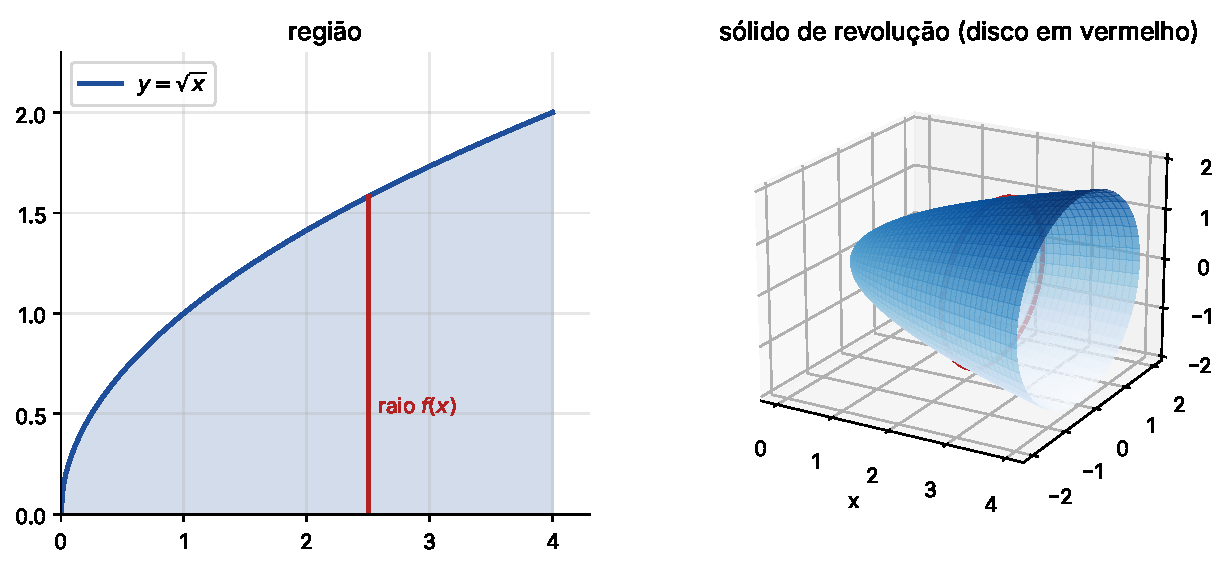
\includegraphics[width=0.8\linewidth]{aula09-revolucao}
\caption{Região sob $y=\sqrt{x}$, $0\le x\le4$, e o sólido obtido ao girá-la em torno do eixo $x$ (um paraboloide).}
\end{figure}

\begin{entrada}
V = sp.pi * sp.integrate(sp.sqrt(x)**2, (x, 0, 4))
V
\end{entrada}
\begin{saidamat}
$\displaystyle 8 \pi$
\end{saidamat}

Com um raio simbólico, deduzimos o volume da esfera girando o semicírculo $y=\sqrt{r^2-x^2}$:

\begin{entrada}
r = sp.symbols('r', positive=True)
sp.pi * sp.integrate(sp.sqrt(r**2 - x**2)**2, (x, -r, r))
\end{entrada}
\begin{saidamat}
$\displaystyle \frac{4 \pi r^{3}}{3}$
\end{saidamat}

\paragraph{Comprimento de arco.} O comprimento do gráfico de $f$ entre $a$ e $b$ é
$\int_a^b\sqrt{1+f'(x)^2}\,dx$. Para $y=\frac23x^{3/2}$, $0\le x\le3$:

\begin{entrada}
f = sp.Rational(2, 3) * x**sp.Rational(3, 2)
sp.integrate(sp.sqrt(1 + sp.diff(f, x)**2), (x, 0, 3))
\end{entrada}
\begin{saidamat}
$\displaystyle \frac{14}{3}$
\end{saidamat}

% ------------------------------------------------------------
\section{Integrais duplas}
% ------------------------------------------------------------

Integrais iteradas são feitas indicando várias variáveis, \textbf{da mais interna para a mais externa}:
\py{sp.integrate(f, (y, c, d), (x, a, b))} calcula $\int_a^b\!\left(\int_c^d f\,dy\right)dx$.

\begin{entrada}
sp.integrate(x*y**2, (y, 0, 2), (x, 0, 3))         # retângulo [0,3] x [0,2]
\end{entrada}
\begin{saidamat}
$\displaystyle 12$
\end{saidamat}

Em uma região do tipo $\{(x,y): a\le x\le b,\ g_1(x)\le y\le g_2(x)\}$, os limites da integral interna dependem
de $x$. Por exemplo, a região entre $y=x^2$ e $y=x$:

\begin{entrada}
sp.integrate(x + y, (y, x**2, x), (x, 0, 1))
\end{entrada}
\begin{saidamat}
$\displaystyle \frac{3}{20}$
\end{saidamat}

A área de uma região é a integral dupla de 1. Em coordenadas polares, $dA=r\,dr\,d\theta$: a área do círculo de raio
$R$ é

\begin{entrada}
rho, theta, R = sp.symbols('rho theta R', positive=True)
sp.integrate(rho, (rho, 0, R), (theta, 0, 2*sp.pi))
\end{entrada}
\begin{saidamat}
$\displaystyle \pi R^{2}$
\end{saidamat}

\begin{professor}
A comparação ``errado \emph{versus} certo'' na área entre seno e cosseno costuma gerar uma boa discussão. Se a
turma ainda não viu integrais duplas, a última seção pode ser omitida ou apenas mostrada. Uma atividade
alternativa é retomar a regra dos trapézios da Aula 4 e compará-la com o valor exato do SymPy.
\end{professor}

% ------------------------------------------------------------
\section{Exercícios}
% ------------------------------------------------------------

\begin{exercicio}[primitivas]{ex:9-primitivas}
Calcule e confira derivando: (a) $\int x^2e^{-x}\,dx$; (b) $\int\frac{x+3}{x^2+x-2}\,dx$; (c) $\int\sec^2 x\,dx$;
(d) $\int x\ln x\,dx$; (e) $\int\frac{dx}{1+4x^2}$.
\end{exercicio}

\begin{exercicio}[definidas e impróprias]{ex:9-definidas}
Calcule: (a) $\int_0^{\pi/2}\sin^2x\,dx$; (b) $\int_1^e\frac{\ln x}{x}\,dx$; (c) $\int_0^\infty xe^{-x}\,dx$;
(d) $\int_0^1\frac{dx}{\sqrt x}$; (e) $\int_0^1 \frac{dx}{x}$.
\end{exercicio}

\begin{exercicio}[área]{ex:9-area}
Calcule a área da região limitada por $y=x^3-x$ e $y=3x$ e faça um gráfico da região.
\end{exercicio}

\begin{exercicio}[Riemann]{ex:9-riemann}
Para $f(x)=\sqrt{x}$ em $[0,4]$, calcule numericamente as somas pela esquerda, direita e ponto médio para
$N=10, 100, 1000$ e compare com o valor exato $\frac{16}{3}$. Qual converge mais rápido?
\end{exercicio}

\begin{exercicio}[volume]{ex:9-volume}
Calcule o volume do sólido obtido girando em torno do eixo $x$ a região sob $y=e^{-x}$, $x\ge0$. Calcule também
o volume do cone obtido girando $y=\frac{R}{h}x$, $0\le x\le h$, e confira que é $\frac13\pi R^2h$.
\end{exercicio}

\begin{exercicio}[extra: valor médio e integral dupla]{ex:9-extra}
(a) O valor médio de $f$ em $[a,b]$ é $\frac{1}{b-a}\int_a^bf$. Calcule o valor médio de $\sin x$ em $[0,\pi]$.
(b) Calcule $\iint_D xy\,dA$, em que $D$ é o triângulo de vértices $(0,0)$, $(1,0)$ e $(1,1)$.
\end{exercicio}

% ============================================================
\chapter{SymPy IV: matrizes simbólicas e equações diferenciais}
\label{cap:aula10}
% ============================================================

\begin{objetivos}
\begin{itemize}
  \item trabalhar com matrizes exatas no SymPy: determinante, inversa, escalonamento (\py{rref}), posto, núcleo,
        autovalores, autovetores e diagonalização;
  \item discutir sistemas lineares com parâmetros;
  \item resolver equações diferenciais ordinárias com \py{sp.dsolve}, com e sem condições iniciais;
  \item visualizar campos de direções e soluções; conhecer a solução numérica de sistemas (\emph{extra}).
\end{itemize}
\end{objetivos}

\begin{roteiro}
0--25 min & \py{sp.Matrix}: operações exatas, \py{det}, \py{inv}, \py{rref}, \py{rank}, \py{nullspace}.\\
25--40 min & Autovalores, autovetores e diagonalização; sistemas com parâmetros.\\
40--65 min & EDOs com \py{dsolve}: 1ª e 2ª ordem, condições iniciais, verificação.\\
65--75 min & Campo de direções; gráfico de soluções.\\
75--90 min & Atividade de encerramento do curso.\\
\end{roteiro}

\begin{entrada}
import sympy as sp
import numpy as np
import matplotlib.pyplot as plt
x, y, z, t = sp.symbols('x y z t')
\end{entrada}

% ------------------------------------------------------------
\section{Matrizes no SymPy}
% ------------------------------------------------------------

Na Aula 5 usamos o NumPy, que faz contas \emph{aproximadas}. O \py{sp.Matrix} faz contas \emph{exatas}, com frações,
raízes e símbolos, como a função \texttt{matrix} do Maxima.

\begin{entrada}
A = sp.Matrix([[1, 2], [-3, 1]])
B = sp.Matrix([[2], [4]])
C = sp.Matrix([[2, 5], [4, 10]])
A, B, C
\end{entrada}
\begin{saidamat}
$\displaystyle \left( \left[\begin{matrix}1 & 2\\-3 & 1\end{matrix}\right], \  \left[\begin{matrix}2\\4\end{matrix}\right], \  \left[\begin{matrix}2 & 5\\4 & 10\end{matrix}\right]\right)$
\end{saidamat}

\begin{atencao}
No SymPy, \py{A * B} é o \textbf{produto de matrizes} (no NumPy era elemento a elemento) e \py{A**n} é a potência
de matrizes. \py{A @ B} também funciona nos dois.
\end{atencao}

\begin{center}\small
\begin{tabular}{@{}lll@{}}
\toprule
\textbf{Matemática} & \textbf{SymPy} & \textbf{Maxima}\\
\midrule
$AB$, $A^n$, $A^T$ & \py{A*B}, \py{A**n}, \py{A.T} & \texttt{A.B}, \texttt{A\^{}\^{}n}, \texttt{transpose(A)}\\
$\det A$, $A^{-1}$ & \py{A.det()}, \py{A.inv()} ou \py{A**-1} & \texttt{determinant(A)}, \texttt{invert(A)}\\
forma escalonada reduzida & \py{A.rref()} & \texttt{echelon(A)} (escalonada)\\
posto, núcleo & \py{A.rank()}, \py{A.nullspace()} & \texttt{rank(A)}, \texttt{nullspace(A)}\\
autovalores, autovetores & \py{A.eigenvals()}, \py{A.eigenvects()} & \texttt{eigenvalues(A)}, \texttt{eigenvectors(A)}\\
polinômio característico & \py{A.charpoly(x)} & \texttt{charpoly(A, x)}\\
identidade, nula & \py{sp.eye(n)}, \py{sp.zeros(m, n)} & \texttt{ident(n)}, \texttt{zeromatrix(m,n)}\\
\bottomrule
\end{tabular}
\end{center}

\begin{entrada}
A*B, A*C - C*A, A.det(), A.inv()
\end{entrada}
\begin{saidamat}
$\displaystyle \left( \left[\begin{matrix}10\\-2\end{matrix}\right], \  \left[\begin{matrix}23 & 16\\24 & -23\end{matrix}\right], \  7, \  \left[\begin{matrix}\frac{1}{7} & - \frac{2}{7}\\\frac{3}{7} & \frac{1}{7}\end{matrix}\right]\right)$
\end{saidamat}

Compare com a Aula 5: o determinante é exatamente 7 e a inversa tem frações exatas.

\paragraph{Matrizes com símbolos.} Podemos obter fórmulas gerais:

\begin{entrada}
a, b, c, d = sp.symbols('a b c d')
M = sp.Matrix([[a, b], [c, d]])
M.det(), M.inv()
\end{entrada}
\begin{saidamat}
$\displaystyle \left( a d - b c, \  \left[\begin{matrix}\frac{d}{a d - b c} & - \frac{b}{a d - b c}\\- \frac{c}{a d - b c} & \frac{a}{a d - b c}\end{matrix}\right]\right)$
\end{saidamat}

\begin{entrada}
k = sp.symbols('k')
K = sp.Matrix([[1, 2, 3], [0, k, 1], [2, 4, k]])
dK = sp.factor(K.det())
print("det =", dK, "   singular para k =", sp.solve(dK, k))
\end{entrada}
\begin{saida}
det = k*(k - 6)    singular para k = [0, 6]
\end{saida}

\paragraph{Escalonamento.} O método \py{rref()} devolve a forma escalonada reduzida e as colunas dos pivôs. Aplicado
à matriz ampliada de um sistema, resolve o sistema ``à mão'', como em Álgebra Linear:

\begin{entrada}
Ab = sp.Matrix([[1, 1, -2, 1],
                [1, 1, -1, 3],
                [3, 1, -1, 3]])       # sistema x+y-2z=1, x+y-z=3, 3x+y-z=3
Ab.rref()
\end{entrada}
\begin{saidamat}
$\displaystyle \left( \left[\begin{matrix}1 & 0 & 0 & 0\\0 & 1 & 0 & 5\\0 & 0 & 1 & 2\end{matrix}\right], \  \left( 0, \  1, \  2\right)\right)$
\end{saidamat}

A última coluna dá a solução $x=0$, $y=5$, $z=2$ (a mesma das Aulas 5 e 7).

\paragraph{Sistemas com parâmetro.} Para que valores de $k$ o sistema
$\begin{cases}x+2y+3z=1\\ ky+z=2\\ 2x+4y+kz=3\end{cases}$ tem solução única? Pelo cálculo acima, $\det K=k(k-6)$:
há solução única para $k\neq0$ e $k\neq6$. Nos casos $k=0$ e $k=6$, comparamos os postos:

\begin{entrada}
bvec = sp.Matrix([1, 2, 3])
for kv in [0, 6]:
    Kk = K.subs(k, kv)
    ampliada = Kk.row_join(bvec)
    print(f"k = {kv}: posto(K) = {Kk.rank()}, posto(ampliada) = {ampliada.rank()}")
sp.simplify(K.LUsolve(bvec))           # solução para k diferente de 0 e 6
\end{entrada}
\begin{saida}
k = 0: posto(K) = 2, posto(ampliada) = 3
k = 6: posto(K) = 2, posto(ampliada) = 3
\end{saida}
\begin{saidamat}
$\displaystyle \left[\begin{matrix}\frac{k^{2} - 13 k + 26}{k \left(k - 6\right)}\\\frac{2 k - 13}{k \left(k - 6\right)}\\\frac{1}{k - 6}\end{matrix}\right]$
\end{saidamat}

Para $k=0$ e $k=6$ os postos são diferentes: o sistema é impossível.

\paragraph{Núcleo, imagem e autovetores.}

\begin{entrada}
C.nullspace(), C.columnspace(), C.rank()
\end{entrada}
\begin{saidamat}
$\displaystyle \left( \left[ \left[\begin{matrix}- \frac{5}{2}\\1\end{matrix}\right]\right], \  \left[ \left[\begin{matrix}2\\4\end{matrix}\right]\right], \  1\right)$
\end{saidamat}

\begin{entrada}
M = sp.Matrix([[3, 0, 0], [0, 3, 0], [0, 1, 1]])
print(M.charpoly(x).as_expr(), "  autovalores:", M.eigenvals())
M.eigenvects()
\end{entrada}
\begin{saida}
x**3 - 7*x**2 + 15*x - 9   autovalores: {3: 2, 1: 1}
\end{saida}
\begin{saidamat}
$\displaystyle \left[ \left( 1, \  1, \  \left[ \left[\begin{matrix}0\\0\\1\end{matrix}\right]\right]\right), \  \left( 3, \  2, \  \left[ \left[\begin{matrix}1\\0\\0\end{matrix}\right], \  \left[\begin{matrix}0\\2\\1\end{matrix}\right]\right]\right)\right]$
\end{saidamat}

A saída de \py{eigenvals()} é um dicionário \{autovalor: multiplicidade\}; a de \py{eigenvects()} é uma lista de
triplas (autovalor, multiplicidade, lista de autovetores). Como há 3 autovetores independentes, $M$ é diagonalizável:

\begin{entrada}
P, D = M.diagonalize()
P, D, P*D*P.inv() == M
\end{entrada}
\begin{saidamat}
$\displaystyle \left( \left[\begin{matrix}0 & 1 & 0\\0 & 0 & 2\\1 & 0 & 1\end{matrix}\right], \  \left[\begin{matrix}1 & 0 & 0\\0 & 3 & 0\\0 & 0 & 3\end{matrix}\right], \  \text{True}\right)$
\end{saidamat}

\paragraph{Aplicação: reconhecimento de cônicas.} A parte quadrática de $ax^2+bxy+cy^2+dx+ey+f=0$ é
$\begin{pmatrix}x&y\end{pmatrix}Q\begin{pmatrix}x\\y\end{pmatrix}$ com $Q=\begin{pmatrix}a&b/2\\b/2&c\end{pmatrix}$. Os
sinais dos autovalores de $Q$ dizem o tipo da cônica (mesmo sinal: elipse; sinais opostos: hipérbole; um nulo:
parábola, salvo casos degenerados). Para a cônica $x^2+2xy-3y^2+x+2y-4=0$ desenhada na Aula 6:

\begin{entrada}
Q = sp.Matrix([[1, sp.Rational(2, 2)], [sp.Rational(2, 2), -3]])
Q.eigenvals()
\end{entrada}
\begin{saidamat}
$\displaystyle \left\{ -1 + \sqrt{5} : 1, \  - \sqrt{5} - 1 : 1\right\}$
\end{saidamat}

Os autovalores $-1\pm\sqrt5$ têm sinais opostos: é uma hipérbole, como no gráfico.

% ------------------------------------------------------------
\section{Equações diferenciais ordinárias}
% ------------------------------------------------------------

Uma equação diferencial envolve uma função desconhecida e suas derivadas. No SymPy, a função desconhecida é
declarada com \py{sp.Function}, a derivada $y'(t)$ é escrita \py{y(t).diff(t)} e a equação é resolvida com
\py{sp.dsolve}.

\begin{sintaxe}
y = sp.Function('y')
edo = sp.Eq(y(t).diff(t), ...)              # ou uma expressão igualada a zero
sp.dsolve(edo, y(t))                        # solução geral
sp.dsolve(edo, y(t), ics={y(0): 1})         # problema de valor inicial
\end{sintaxe}

\subsection{Primeira ordem}

\paragraph{Crescimento exponencial.} $y'=ky$:

\begin{entrada}
y = sp.Function('y')
k = sp.symbols('k')
sp.dsolve(sp.Eq(y(t).diff(t), k*y(t)), y(t))
\end{entrada}
\begin{saidamat}
$\displaystyle y{\left(t \right)} = C_{1} e^{k t}$
\end{saidamat}

A constante arbitrária aparece como $C_1$. Com uma condição inicial, ela é determinada:

\begin{entrada}
sol = sp.dsolve(sp.Eq(y(t).diff(t), k*y(t)), y(t), ics={y(0): 100})
sol
\end{entrada}
\begin{saidamat}
$\displaystyle y{\left(t \right)} = 100 e^{k t}$
\end{saidamat}

O lado direito da solução, \py{sol.rhs}, é uma expressão comum, que pode ser avaliada, derivada ou desenhada:

\begin{entrada}
print(sol.rhs.subs({k: sp.log(2)/3, t: 6}))     # se a população dobra a cada 3 horas
\end{entrada}
\begin{saida}
400
\end{saida}

\paragraph{Equação linear de primeira ordem.} $y'+2y=e^{t}$, $y(0)=1$:

\begin{entrada}
edo = sp.Eq(y(t).diff(t) + 2*y(t), sp.exp(t))
sp.dsolve(edo, y(t), ics={y(0): 1})
\end{entrada}
\begin{saidamat}
$\displaystyle y{\left(t \right)} = \frac{e^{t}}{3} + \frac{2 e^{- 2 t}}{3}$
\end{saidamat}

\paragraph{Equação separável e equação logística.} $y'=t\,y^2$ e $P'=rP\left(1-\frac{P}{K}\right)$:

\begin{entrada}
sp.dsolve(sp.Eq(y(t).diff(t), t*y(t)**2), y(t))
\end{entrada}
\begin{saidamat}
$\displaystyle y{\left(t \right)} = - \frac{2}{C_{1} + t^{2}}$
\end{saidamat}

\begin{entrada}
P = sp.Function('P')
r, K = sp.symbols('r K', positive=True)
log_sol = sp.dsolve(sp.Eq(P(t).diff(t), r*P(t)*(1 - P(t)/K)), P(t), ics={P(0): 10})
sp.simplify(log_sol)
\end{entrada}
\begin{saidamat}
$\displaystyle P{\left(t \right)} = \frac{10 K e^{r t}}{K + 10 e^{r t} - 10}$
\end{saidamat}

\paragraph{Verificando a solução.} O comando \py{sp.checkodesol} substitui a solução na equação; a resposta
\py{(True, 0)} confirma que ela está correta.

\begin{entrada}
sp.checkodesol(edo, sp.dsolve(edo, y(t)))
\end{entrada}
\begin{saidamat}
$\displaystyle \left( \text{True}, \  0\right)$
\end{saidamat}

\subsection{Segunda ordem}

A segunda derivada é \py{y(t).diff(t, 2)}. Equação $g''-2g'+g=0$ (raiz dupla da equação característica):

\begin{entrada}
g = sp.Function('g')
sp.dsolve(g(t).diff(t, 2) - 2*g(t).diff(t) + g(t), g(t))
\end{entrada}
\begin{saidamat}
$\displaystyle g{\left(t \right)} = \left(C_{1} + C_{2} t\right) e^{t}$
\end{saidamat}

\paragraph{Oscilador harmônico.} $x''+\omega^2x=0$ com $x(0)=1$, $x'(0)=0$. A condição sobre a derivada é escrita
\py{x(t).diff(t).subs(t, 0)}:

\begin{entrada}
X = sp.Function('X')
w = sp.symbols('omega', positive=True)
sp.dsolve(X(t).diff(t, 2) + w**2*X(t), X(t), ics={X(0): 1, X(t).diff(t).subs(t, 0): 0})
\end{entrada}
\begin{saidamat}
$\displaystyle X{\left(t \right)} = \cos{\left(\omega t \right)}$
\end{saidamat}

\paragraph{Uma equação não homogênea} (tutorial do R. Miranda): $q''-6q'+2q=t\cos t$, com $q(0)=1$, $q'(0)=1$. A
solução é longa, mas o gráfico é imediato com \py{sp.plot}:

% figura: aula10-naohomog
\begin{entrada}
q = sp.Function('q')
edo2 = q(t).diff(t, 2) - 6*q(t).diff(t) + 2*q(t) - t*sp.cos(t)
solucao = sp.dsolve(edo2, q(t), ics={q(0): 1, q(t).diff(t).subs(t, 0): 1})
sp.plot(solucao.rhs, (t, -2, 2), ylim=(-5, 5), ylabel="q(t)")
\end{entrada}
\saidafig[0.55]{aula10-naohomog}

\begin{maxima}
No Maxima: \texttt{ode2('diff(y,t) = k*y, y, t)} e, para condições iniciais, \texttt{ic1} e \texttt{ic2}
(ou \texttt{desolve} com \texttt{atvalue}). No SymPy tudo é feito com \py{sp.dsolve(..., ics={...})}. Note que no
Maxima a derivada da incógnita é escrita com apóstrofo, \texttt{'diff(y,t)}; no SymPy é \py{y(t).diff(t)}.
\end{maxima}

\subsection{Campo de direções}

Para $y'=F(t,y)$, em cada ponto $(t,y)$ desenhamos um pequeno segmento com inclinação $F(t,y)$. As soluções são
curvas tangentes a esses segmentos. O comando \py{plt.quiver} desenha setas em uma malha. Exemplo:
$y'=y(1-y)$ (logística com $r=K=1$), com algumas soluções.

% figura: aula10-campo
\begin{entrada}
F = lambda T, Y: Y*(1 - Y)
T, Y = np.meshgrid(np.linspace(0, 6, 22), np.linspace(-0.5, 2, 18))
U, V = np.ones_like(T), F(T, Y)
N = np.sqrt(U**2 + V**2)                      # normaliza as setas
plt.quiver(T, Y, U/N, V/N, angles="xy", color="gray", width=0.003)

ts = np.linspace(0, 6, 200)
for y0 in [0.05, 0.3, 1.0, 1.5, 2.0]:
    sol = sp.dsolve(sp.Eq(y(t).diff(t), y(t)*(1 - y(t))), y(t), ics={y(0): y0})
    plt.plot(ts, sp.lambdify(t, sol.rhs)(ts) * np.ones_like(ts), lw=2, label=f"y(0) = {y0}")
plt.ylim(-0.5, 2)
plt.xlabel("t"); plt.ylabel("y")
plt.legend(loc="lower right", fontsize=8)
plt.show()
\end{entrada}
\saidafig[0.6]{aula10-campo}

As soluções com $y(0)>0$ tendem a $y=1$ (equilíbrio estável); $y=0$ é um equilíbrio instável.

\subsection{Extra: sistemas e soluções numéricas}

O \py{dsolve} encontra soluções \emph{exatas}, que nem sempre existem. Para sistemas não lineares, como o famoso
sistema de Lorenz
\[
\dot x=\sigma(y-x),\qquad \dot y=x(\rho-z)-y,\qquad \dot z=xy-\beta z,
\]
usa-se um método numérico, como o \py{solve_ivp} da biblioteca SciPy (tutorial do R. Miranda):

% figura: aula10-lorenz
\begin{entrada}
from scipy.integrate import solve_ivp

def lorenz(t, u, sigma=10, rho=28, beta=8/3):
    x, y, z = u
    return [sigma*(y - x), x*(rho - z) - y, x*y - beta*z]

sol = solve_ivp(lorenz, (0, 40), [1, 1, 1], max_step=0.01)
ax = plt.figure(figsize=(6, 5)).add_subplot(projection="3d")
ax.plot(sol.y[0], sol.y[1], sol.y[2], lw=0.5)
ax.set_title("Atrator de Lorenz")
plt.show()
\end{entrada}
\saidafig[0.5]{aula10-lorenz}

% ------------------------------------------------------------
\section{Atividade de encerramento}
% ------------------------------------------------------------

Sugestão para a parte final da aula (ou como trabalho): em duplas, cada grupo escolhe \textbf{um} dos temas abaixo e
produz um notebook com texto explicativo (células Markdown), código e pelo menos um gráfico.

\begin{enumerate}
  \item \textbf{Estudo completo de uma função}: domínio, limites, assíntotas, derivadas, extremos, inflexões e
  gráfico (Aulas 6 e 8).
  \item \textbf{Aproximações de $\pi$}: série de Leibniz, Monte Carlo, área do círculo por somas de Riemann e por
  trapézios; comparar velocidades de convergência (Aulas 3, 4 e 9).
  \item \textbf{Métodos para equações}: bissecção, método babilônico/Newton e \py{nsolve}; comparar número de
  passos (Aulas 3 e 7).
  \item \textbf{Cônicas}: dada $ax^2+bxy+cy^2+dx+ey+f=0$, classificar pelos autovalores e desenhar (Aulas 6 e 10).
  \item \textbf{Modelos populacionais}: crescimento exponencial e logístico; ajuste de parâmetros a dados reais
  (por exemplo, população brasileira nos censos) com \py{np.polyfit} e \py{dsolve} (Aulas 5 e 10).
\end{enumerate}

\begin{professor}
Esta aula concentra muito conteúdo; se necessário, a parte de matrizes pode ser apenas apresentada (os alunos já
viram NumPy na Aula 5) e o foco ficar nas EDOs. O exemplo de Lorenz requer a SciPy; se ela não estiver instalada
nas máquinas, mostre-o projetado. A atividade de encerramento pode substituir uma avaliação ou servir como
revisão.
\end{professor}

% ------------------------------------------------------------
\section{Exercícios}
% ------------------------------------------------------------

\begin{exercicio}[matrizes]{ex:10-mat}
Para $A=\begin{pmatrix}2&-1&0\\-1&2&-1\\0&-1&2\end{pmatrix}$, calcule de forma exata: $\det A$, $A^{-1}$, o
polinômio característico, os autovalores e os autovetores. Verifique que $A$ é diagonalizável.
\end{exercicio}

\begin{exercicio}[sistema com parâmetro]{ex:10-param}
Discuta, em função de $a$, o sistema $\begin{cases}x+y+z=1\\x+ay+z=2\\x+y+az=3\end{cases}$: para que valores há
solução única? Para os demais valores, o sistema é impossível ou indeterminado?
\end{exercicio}

\begin{exercicio}[EDOs de primeira ordem]{ex:10-edo1}
Resolva e verifique com \py{checkodesol}: (a) $y'=-2ty$, $y(0)=1$; (b) $y'+y=t$; (c) $y'=\frac{y}{t}+t$.
\end{exercicio}

\begin{exercicio}[lei do resfriamento]{ex:10-resfriamento}
Pela lei de Newton, a temperatura de um café satisfaz $T'=-k(T-25)$. Se $T(0)=90$ e $T(5)=70$ (minutos, °C),
encontre $k$ e o instante em que o café chega a $40$\,°C. Faça o gráfico de $T(t)$.
\end{exercicio}

\begin{exercicio}[segunda ordem]{ex:10-edo2}
Resolva $y''+y'+y=0$ com $y(0)=1$, $y'(0)=0$ (oscilador amortecido) e faça o gráfico para $t\in[0,15]$.
Compare com $y''+y=0$ com as mesmas condições iniciais.
\end{exercicio}

\begin{exercicio}[extra: campo de direções]{ex:10-campo}
Desenhe o campo de direções de $y'=t-y$ em $[-2,3]\times[-2,3]$ e algumas soluções obtidas com \py{dsolve}. Que reta
é solução da equação?
\end{exercicio}


\appendix
% ============================================================
\chapter{Do Maxima para o Python}
\label{ap:maxima}
% ============================================================

Esta tabela ajuda a adaptar as atividades feitas com o Maxima. Supõe-se que foram executados
\py{import sympy as sp}, \py{import numpy as np}, \py{import matplotlib.pyplot as plt} e
\py{x, y, t = sp.symbols('x y t')}.

\begin{center}\small
\renewcommand{\arraystretch}{1.18}
\begin{longtable}{@{}>{\raggedright\arraybackslash}p{3.3cm}>{\raggedright\arraybackslash}p{5.3cm}>{\raggedright\arraybackslash}p{5.6cm}@{}}
\toprule
\textbf{Tarefa} & \textbf{Maxima} & \textbf{Python (SymPy/NumPy)}\\
\midrule
\endhead
\multicolumn{3}{@{}l}{\textbf{\sffamily Básico}}\\
atribuição & \texttt{a: 5;} & \py{a = 5}\\
definir função & \texttt{f(x) := x\^{}2 + 1;} & \py{def f(x): return x**2 + 1} ou \py{f = x**2 + 1} (expressão)\\
avaliar & \texttt{f(2);} \ \texttt{ev(e, x=2);} \ \texttt{subst(2, x, e);} & \py{f(2)} \ ou \ \py{e.subs(x, 2)}\\
potência & \texttt{x\^{}2} ou \texttt{x**2} & \py{x**2} (\textbf{nunca} \py{x^2})\\
constantes & \texttt{\%pi}, \texttt{\%e}, \texttt{\%i}, \texttt{inf} & \py{sp.pi}, \py{sp.E}, \py{sp.I}, \py{sp.oo}\\
valor numérico & \texttt{float(e);} \ \texttt{bfloat(e), fpprec:50;} & \py{e.evalf()} \ \ \py{sp.N(e, 50)}\\
fração exata & \texttt{1/3} & \py{sp.Rational(1, 3)} (\py{1/3} é \py{float})\\
último resultado & \texttt{\%} & \py{_} (no Jupyter)\\
listas & \texttt{L: [1, 2, 3]; L[1];} & \py{L = [1, 2, 3]}; \py{L[0]} (começa em 0)\\
gerar lista & \texttt{makelist(k\^{}2, k, 1, 10);} & \py{[k**2 for k in range(1, 11)]}\\
soma de lista & \texttt{apply("+", L);} \ \texttt{lsum(k, k, L);} & \py{sum(L)}\\
\multicolumn{3}{@{}l}{\textbf{\sffamily Álgebra}}\\
expandir & \texttt{expand(e);} & \py{sp.expand(e)}\\
fatorar & \texttt{factor(e);} & \py{sp.factor(e)}\\
simplificar & \texttt{ratsimp(e);} \ \texttt{fullratsimp(e);} & \py{sp.simplify(e)}, \py{sp.cancel(e)}\\
trigonometria & \texttt{trigsimp}, \texttt{trigexpand}, \texttt{trigreduce} & \py{sp.trigsimp}, \py{sp.expand_trig}, \py{sp.fu}\\
frações parciais & \texttt{partfrac(e, x);} & \py{sp.apart(e, x)}\\
agrupar & \texttt{collectterms(e, x);} & \py{sp.collect(e, x)}\\
numerador, denominador & \texttt{num(e)}, \texttt{denom(e)} & \py{sp.numer(e)}, \py{sp.denom(e)}\\
divisão de polinômios & \texttt{divide(p, q, x);} & \py{sp.div(p, q, x)}\\
hipóteses & \texttt{assume(a > 0);} & \py{a = sp.symbols('a', positive=True)}\\
\multicolumn{3}{@{}l}{\textbf{\sffamily Equações}}\\
resolver & \texttt{solve(x\^{}2 = 4, x);} & \py{sp.solve(sp.Eq(x**2, 4), x)} ou \py{sp.solve(x**2 - 4, x)}\\
sistema & \texttt{solve([eq1, eq2], [x, y]);} & \py{sp.solve([eq1, eq2], [x, y], dict=True)}\\
sistema linear & \texttt{linsolve([eq1, eq2], [x, y]);} & \py{sp.linsolve([eq1, eq2], [x, y])}\\
raízes numéricas & \texttt{allroots(p);} \ \texttt{realroots(p);} & \py{sp.Poly(p, x).nroots()}, \py{sp.real_roots(p)}, \py{np.roots(coef)}\\
raiz numérica & \texttt{find\_root(f, x, a, b);} & \py{sp.nsolve(f, x, chute)}\\
inequação & \texttt{fourier\_elim} / \texttt{solve\_rat\_ineq} & \py{sp.solveset(x**2 > 4, x, sp.S.Reals)}\\
lado direito & \texttt{rhs(eq);} & \py{eq.rhs}\\
\multicolumn{3}{@{}l}{\textbf{\sffamily Cálculo}}\\
limite & \texttt{limit(f, x, 0);} & \py{sp.limit(f, x, 0, '+-')} (sem \py{'+-'}: pela direita)\\
limite lateral & \texttt{limit(f, x, 0, plus);} \ \texttt{minus} & \py{sp.limit(f, x, 0, '+')}, \py{'-'}\\
derivada & \texttt{diff(f, x);} \ \texttt{diff(f, x, 2);} & \py{sp.diff(f, x)}, \py{sp.diff(f, x, 2)}\\
derivada parcial mista & \texttt{diff(f, x, 1, y, 1);} & \py{sp.diff(f, x, y)}\\
derivada em ponto & \texttt{at(diff(f,x), x=a);} & \py{sp.diff(f, x).subs(x, a)}\\
primitiva & \texttt{integrate(f, x);} & \py{sp.integrate(f, x)}\\
integral definida & \texttt{integrate(f, x, a, b);} & \py{sp.integrate(f, (x, a, b))}\\
integral numérica & \texttt{quad\_qags(f, x, a, b);} & \py{sp.Integral(f, (x, a, b)).evalf()}\\
somatório & \texttt{sum(k\^{}2, k, 1, n), simpsum;} & \py{sp.summation(k**2, (k, 1, n))}\\
Taylor & \texttt{taylor(f, x, 0, 5);} & \py{sp.series(f, x, 0, 6)}\\
EDO & \texttt{ode2('diff(y,x) = x*y, y, x);} & \py{sp.dsolve(sp.Eq(y(x).diff(x), x*y(x)), y(x))}\\
condição inicial & \texttt{ic1(sol, x=0, y=1);} \ \texttt{ic2(...)} & \py{sp.dsolve(..., ics={y(0): 1})}\\
\multicolumn{3}{@{}l}{\textbf{\sffamily Matrizes}}\\
criar & \texttt{A: matrix([1,2],[3,4]);} & \py{A = sp.Matrix([[1, 2], [3, 4]])} ou \py{np.array(...)}\\
elemento & \texttt{A[1,2]} & \py{A[0, 1]} (começa em 0)\\
produto & \texttt{A . B} & \py{A * B} (SymPy), \py{A @ B} (NumPy e SymPy)\\
transposta, inversa & \texttt{transpose(A)}, \texttt{invert(A)}, \texttt{A\^{}\^{}-1} & \py{A.T}, \py{A.inv()}\\
determinante & \texttt{determinant(A);} & \py{A.det()} (SymPy), \py{np.linalg.det(A)}\\
escalonar & \texttt{echelon(A);} & \py{A.rref()}\\
posto, núcleo & \texttt{rank(A)}, \texttt{nullspace(A)} & \py{A.rank()}, \py{A.nullspace()}\\
autovalores & \texttt{eigenvalues(A);} \ \texttt{eigenvectors(A);} & \py{A.eigenvals()}, \py{A.eigenvects()}\\
identidade & \texttt{ident(n)} & \py{sp.eye(n)}, \py{np.eye(n)}\\
\multicolumn{3}{@{}l}{\textbf{\sffamily Gráficos}}\\
função & \texttt{plot2d(f, [x, a, b]);} & \py{sp.plot(f, (x, a, b))} ou Matplotlib\\
várias funções & \texttt{plot2d([f, g], [x, a, b]);} & \py{sp.plot(f, g, (x, a, b))}\\
paramétrica & \texttt{plot2d([parametric, cos(t), sin(t), [t,0,2*\%pi]]);} & \py{sp.plot_parametric(sp.cos(t), sp.sin(t), (t, 0, 2*sp.pi))}\\
implícita & \texttt{implicit\_plot(x\^{}2+y\^{}2=1, [x,-2,2], [y,-2,2]);} & \py{sp.plot_implicit(sp.Eq(x**2 + y**2, 1))}\\
superfície & \texttt{plot3d(f, [x,a,b], [y,c,d]);} & \py{from sympy.plotting import plot3d}; \py{plot3d(f, (x, a, b), (y, c, d))}\\
pontos & \texttt{plot2d([discrete, xs, ys]);} & \py{plt.plot(xs, ys, "o")}\\
\bottomrule
\end{longtable}
\end{center}

\section*{Diferenças que mais causam erros}

\begin{enumerate}
  \item \textbf{Índices começam em 0} no Python e em 1 no Maxima.
  \item \textbf{Símbolos precisam ser declarados} no SymPy: \py{x = sp.symbols('x')}.
  \item \textbf{Frações}: \py{1/3} é um número decimal. Use \py{sp.Rational(1, 3)} quando quiser exatidão.
  \item \textbf{Potência}: \py{**}; o \py{^} não é potência.
  \item \textbf{Integral definida}: os limites vão em uma tupla, \py{(x, a, b)}.
  \item \textbf{Limite sem direção}: no SymPy é pela direita; use \py{'+-'} para o bilateral.
  \item \textbf{Prefixos}: \py{sp.sin} (simbólico), \py{np.sin} (vetores numéricos) e \py{math.sin} (um número) são
  funções diferentes; use cada uma no seu contexto.
  \item \textbf{Igualdade}: \py{=} atribui, \py{==} compara, \py{sp.Eq(a, b)} escreve a equação $a=b$.
\end{enumerate}

% ============================================================
\chapter{Referência rápida}
\label{ap:referencia}
% ============================================================

\section*{Python básico (Aulas 1 e 2)}

\begin{multicols}{2}
\begin{codigo}
# entrada e saída
n = int(input("n = "))
x = float(input("x = "))
print("resultado:", x, n)
print(f"{x:.3f}  {x:e}")

# operações
a + b, a - b, a * b, a / b
a // b      # quociente inteiro
a % b       # resto
a ** b      # potência
abs(a), round(a, 2)

# comparação e lógica
==  !=  <  <=  >  >=
and   or   not

# decisão
if cond:
    ...
elif outra:
    ...
else:
    ...
\end{codigo}

\columnbreak

\begin{codigo}
# repetição
for i in range(1, n + 1):
    ...
while cond:
    ...
break, continue

# listas
L = [3, 1, 2]
L[0], L[-1], L[1:3]
L.append(5); L.insert(0, 9)
len(L), sum(L), max(L)
sorted(L), L.copy()
[k**2 for k in range(10)]

# tuplas e dicionários
P = (1, 2);  x, y = P
D = {"a": 1};  D["a"]

# funções
def f(x, a=1):
    return a * x**2
g = lambda x: x + 1
\end{codigo}
\end{multicols}

\section*{Módulo \texttt{math} e NumPy (Aulas 3 a 5)}

\begin{multicols}{2}
\begin{codigo}
import math
math.sqrt(x), math.exp(x)
math.log(x), math.log(x, b)
math.sin(x), math.radians(g)
math.pi, math.e
math.floor(x), math.ceil(x)
math.factorial(n)
math.comb(n, k), math.gcd(a, b)
math.isqrt(n)
\end{codigo}

\columnbreak

\begin{codigo}
import numpy as np
v = np.array([1, 2, 3])
np.arange(a, b, h)
np.linspace(a, b, n)
v * 2, v + v, v @ v
np.sin(v), np.exp(v)
v[v > 0], np.sum(v), v.mean()
np.cumsum(v), np.argmax(v)
\end{codigo}
\end{multicols}

\begin{codigo}
A = np.array([[1, 2], [3, 4]])
A.shape, A[0, 1], A[:, 0], A.T, A @ B
np.linalg.det(A), np.linalg.inv(A), np.linalg.solve(A, b), np.linalg.eig(A)
np.roots([1, -3, 2]), np.polyval(p, x), np.polyfit(x, y, grau)
\end{codigo}

\section*{Matplotlib (Aula 6)}

\begin{codigo}
import matplotlib.pyplot as plt
x = np.linspace(a, b, 400)
plt.plot(x, f(x), "r--", label="f")      # cor/estilo, legenda
plt.title("..."); plt.xlabel("x"); plt.ylabel("y")
plt.xlim(a, b); plt.ylim(c, d); plt.grid(True); plt.legend(); plt.axis("equal")
plt.savefig("figura.png", dpi=200); plt.show()

fig, ax = plt.subplots(1, 2, figsize=(10, 4))   # vários gráficos: ax[0].plot(...)
X, Y = np.meshgrid(x, y); plt.contour(X, Y, Z, levels=[0])   # curvas de nível
ax = plt.figure().add_subplot(projection="3d"); ax.plot_surface(X, Y, Z)
\end{codigo}

\section*{SymPy (Aulas 7 a 10)}

\begin{codigo}
import sympy as sp
x, y = sp.symbols('x y')                       # declarar símbolos
sp.Rational(1, 3), sp.sqrt(2), sp.pi, sp.E, sp.I, sp.oo
e.evalf(20), sp.N(e, 20), e.subs(x, 2), e.subs({x: 1, y: 2})
sp.expand(e), sp.factor(e), sp.simplify(e), sp.apart(e), sp.collect(e, x)
sp.solve(e, x), sp.solve(sp.Eq(a, b), x), sp.solveset(e, x, sp.S.Reals)
sp.linsolve([e1, e2], [x, y]), sp.nsolve(e, x, chute)
sp.limit(f, x, a, '+-'), sp.limit(f, x, sp.oo), sp.diff(f, x, n)
sp.integrate(f, x), sp.integrate(f, (x, a, b)), sp.summation(f, (k, 1, n))
sp.series(f, x, x0, n).removeO()
M = sp.Matrix([[1, 2], [3, 4]]); M.det(), M.inv(), M.rref(), M.eigenvects()
y = sp.Function('y'); sp.dsolve(sp.Eq(y(x).diff(x), y(x)), y(x), ics={y(0): 1})
sp.plot(f, (x, a, b)); sp.lambdify(x, f, "numpy")
\end{codigo}

\section*{Mensagens de erro mais comuns}

\begin{center}\small
\begin{tabularx}{\linewidth}{@{}l>{\raggedright\arraybackslash}X@{}}
\toprule
\textbf{Erro} & \textbf{Causa provável}\\
\midrule
\py{SyntaxError} & faltam dois-pontos, parênteses ou aspas; uso de \py{^}; vírgula decimal\\
\py{IndentationError} & recuo faltando ou inconsistente após \py{if}, \py{for}, \py{def}...\\
\py{NameError: name 'x' is not defined} & variável/símbolo não criado, célula anterior não executada, erro de digitação\\
\py{TypeError} & operação entre tipos incompatíveis (texto + número; \py{math.sin} de um \emph{array})\\
\py{ValueError} & valor inválido: \py{int("3.5")}, \py{math.sqrt(-1)}, limite que não existe\\
\py{IndexError} & índice fora da lista (lembre que começa em 0)\\
\py{ZeroDivisionError} & divisão por zero\\
\py{ModuleNotFoundError} & biblioteca não instalada: \texttt{\%pip install nome}\\
\bottomrule
\end{tabularx}
\end{center}

\ifprofessor
  % ============================================================
\chapter{Soluções dos exercícios}
\label{ap:solucoes}
% ============================================================

As soluções abaixo são \emph{uma} forma de resolver cada exercício; outras soluções corretas são possíveis e
devem ser valorizadas. Todas as saídas mostradas foram obtidas executando os códigos.

\begin{entrada}
import math
import numpy as np
import sympy as sp
import matplotlib.pyplot as plt
\end{entrada}

% ------------------------------------------------------------
\section*{Aula 1}
% ------------------------------------------------------------

\paragraph{Exercício \ref{ex:1-temp}.}
% entradas: 36.5
\begin{entrada}
C = float(input("Temperatura em °C: "))
F = 9/5*C + 32
print(f"{C} °C = {F:.1f} °F")
\end{entrada}
\begin{saida}
Temperatura em °C: 36.5
36.5 °C = 97.7 °F
\end{saida}

\paragraph{Exercício \ref{ex:1-bissexto}.}
\begin{entrada}
for ano in [1900, 2000, 2024, 2025]:
    bissexto = (ano % 4 == 0 and ano % 100 != 0) or ano % 400 == 0
    print(ano, "é bissexto" if bissexto else "não é bissexto")
\end{entrada}
\begin{saida}
1900 não é bissexto
2000 é bissexto
2024 é bissexto
2025 não é bissexto
\end{saida}

\paragraph{Exercício \ref{ex:1-somas}.}
\begin{entrada}
s = 0
for k in range(1, 100, 2):
    s += k
print("(a)", s)

s = 0
for k in range(1, 21):
    s += 1/k**2
print("(b)", s, "  pi^2/6 =", math.pi**2/6)

n = 10
s = 0
for k in range(1, n + 1):
    s += k**3
print("(c)", s, (n*(n + 1)//2)**2)
\end{entrada}
\begin{saida}
(a) 2500
(b) 1.5961632439130233   pi^2/6 = 1.6449340668482264
(c) 3025 3025
\end{saida}

\paragraph{Exercício \ref{ex:1-5000}.}
\begin{entrada}
soma, k = 0, 0
while soma <= 5000:
    k += 1
    soma += k
print("último número somado:", k, "  soma:", soma)
\end{entrada}
\begin{saida}
último número somado: 100   soma: 5050
\end{saida}

\paragraph{Exercício \ref{ex:1-pa}.}
% entradas: 2 | 3 | 6
\begin{entrada}
a1 = float(input("a1 = "))
r = float(input("razão = "))
n = int(input("n = "))
soma = 0
for k in range(n):
    termo = a1 + k*r
    print(termo, end=" ")
    soma += termo
print("\nsoma =", soma, "  fórmula =", n*(a1 + termo)/2)
\end{entrada}
\begin{saida}
a1 = 2
razão = 3
n = 6
2.0 5.0 8.0 11.0 14.0 17.0
soma = 57.0   fórmula = 57.0
\end{saida}

\paragraph{Exercício \ref{ex:1-collatz}.}
\begin{entrada}
for n in [6, 27]:
    passos = 0
    seq = [n]
    while n != 1:
        n = n // 2 if n % 2 == 0 else 3*n + 1
        seq.append(n)
        passos += 1
    print(passos, "passos; maior valor:", max(seq), "; início:", seq[:8])
\end{entrada}
\begin{saida}
8 passos; maior valor: 16 ; início: [6, 3, 10, 5, 16, 8, 4, 2]
111 passos; maior valor: 9232 ; início: [27, 82, 41, 124, 62, 31, 94, 47]
\end{saida}

\paragraph{Exercício \ref{ex:1-divisores}.}
% entradas: 28
\begin{entrada}
n = int(input("n = "))
qtd = 0
for d in range(1, n + 1):
    if n % d == 0:
        print(d, end=" ")
        qtd += 1
print()
print(n, "é primo" if qtd == 2 else "não é primo")
\end{entrada}
\begin{saida}
n = 28
1 2 4 7 14 28
28 não é primo
\end{saida}

% ------------------------------------------------------------
\section*{Aula 2}
% ------------------------------------------------------------

\paragraph{Exercício \ref{ex:2-listas}.}
\begin{entrada}
L = [3, 8, -2, 7, 0, 5, -6, 1]
print(L[2], L[-1])
print([v for v in L if v > 0])
print([v**2 for v in L])
print(sum(L)/len(L), sorted(L, reverse=True))
\end{entrada}
\begin{saida}
-2 1
[3, 8, 7, 5, 1]
[9, 64, 4, 49, 0, 25, 36, 1]
2.0 [8, 7, 5, 3, 1, 0, -2, -6]
\end{saida}

\paragraph{Exercício \ref{ex:2-quadrados}.}
\begin{entrada}
def soma_quadrados(n):
    return sum([k**2 for k in range(1, n + 1)])

print(all(soma_quadrados(n) == n*(n + 1)*(2*n + 1)//6 for n in range(1, 21)))
\end{entrada}
\begin{saida}
True
\end{saida}

\paragraph{Exercício \ref{ex:2-estat}.}
\begin{entrada}
def media(L):
    return sum(L) / len(L)

def desvio(L):
    m = media(L)
    return math.sqrt(sum([(v - m)**2 for v in L]) / len(L))

notas = [9.5, 7.5, 10, 8.0, 6.5]
print(media(notas), desvio(notas))
\end{entrada}
\begin{saida}
8.3 1.2884098726725126
\end{saida}

\paragraph{Exercício \ref{ex:2-gemeos}.}
\begin{entrada}
def eh_primo(n):
    if n < 2:
        return False
    d = 2
    while d*d <= n:
        if n % d == 0:
            return False
        d += 1
    return True

print([(p, p + 2) for p in range(2, 100) if eh_primo(p) and eh_primo(p + 2)])
\end{entrada}
\begin{saida}
[(3, 5), (5, 7), (11, 13), (17, 19), (29, 31), (41, 43), (59, 61), (71, 73)]
\end{saida}

\paragraph{Exercício \ref{ex:2-mdc}.}
\begin{entrada}
def mdc(a, b):
    while b != 0:
        a, b = b, a % b
    return a

def mmc(a, b):
    return a*b // mdc(a, b)

m = 1
for k in range(2, 11):
    m = mmc(m, k)
print(mdc(252, 198), mmc(4, 6), m)
\end{entrada}
\begin{saida}
18 12 2520
\end{saida}

\paragraph{Exercício \ref{ex:2-poli}.}
\begin{entrada}
def avalia(coef, x):
    return sum([a * x**k for k, a in enumerate(coef)])

def deriva(coef):
    return [k * coef[k] for k in range(1, len(coef))]

p = [1, -3, 0, 2]          # 1 - 3x + 2x^3
print(avalia(p, 2), deriva(p), avalia(deriva(p), 2))
\end{entrada}
\begin{saida}
11 [-3, 0, 6] 21
\end{saida}

% ------------------------------------------------------------
\section*{Aula 3}
% ------------------------------------------------------------

\paragraph{Exercício \ref{ex:3-dist}.}
\begin{entrada}
def distancia(P, Q):
    return math.hypot(Q[0] - P[0], Q[1] - P[1])

A, B, C = (0, 0), (4, 0), (1, 3)
print(distancia(A, B) + distancia(B, C) + distancia(C, A))
\end{entrada}
\begin{saida}
11.404918347287664
\end{saida}

\paragraph{Exercício \ref{ex:3-relogio}.}
\begin{entrada}
def angulo(h, m):
    dif = abs((30*h + 0.5*m) - 6*m) % 360
    return min(dif, 360 - dif)

print(angulo(3, 0), angulo(9, 45), angulo(12, 30))
\end{entrada}
\begin{saida}
90.0 22.5 165.0
\end{saida}

\paragraph{Exercício \ref{ex:3-series}.}
\begin{entrada}
for n in [5, 10, 15]:
    s = sum([1/math.factorial(k) for k in range(n + 1)])
    print(n, s, abs(s - math.e))
for n in [10, 1000, 100000]:
    s = 4*sum([(-1)**k/(2*k + 1) for k in range(n + 1)])
    print(n, s, abs(s - math.pi))
\end{entrada}
\begin{saida}
5 2.716666666666667 0.0016151617923783057
10 2.7182818011463845 2.7312660577649694e-08
15 2.7182818284589945 5.062616992290714e-14
10 3.232315809405593 0.09072315581579993
1000 3.1425916543395434 0.000999000749750234
100000 3.141602653489794 9.999900000945416e-06
\end{saida}

A série de $e$ converge muito mais rápido: o erro cai como $\frac{1}{(n+1)!}$, enquanto na de Leibniz cai como
$\frac1n$.

\paragraph{Exercício \ref{ex:3-seno}.}
\begin{entrada}
def seno(x, n):
    return sum([(-1)**k * x**(2*k + 1) / math.factorial(2*k + 1) for k in range(n + 1)])

for x in [1, 10]:
    print(x, seno(x, 5), seno(x, 20), math.sin(x))
\end{entrada}
\begin{saida}
1 0.841470984648068 0.8414709848078965 0.8414709848078965
10 -1056.9392336059002 -0.5440211107317661 -0.5440211108893698
\end{saida}

\paragraph{Exercício \ref{ex:3-cubica}.}
\begin{entrada}
def raiz_cubica(x, tol=1e-12):
    y = x if abs(x) > 1 else 1.0
    while True:
        novo = (2*y + x/y**2) / 3
        if abs(novo - y) < tol:
            return novo
        y = novo

print(raiz_cubica(27), raiz_cubica(2), math.cbrt(2), raiz_cubica(-8))
\end{entrada}
\begin{saida}
3.0 1.2599210498948732 1.2599210498948734 -2.0
\end{saida}

\paragraph{Exercício \ref{ex:3-bissec}.}
\begin{entrada}
def bisseccao(f, a, b, tol=1e-10):
    while (b - a)/2 > tol:
        m = (a + b)/2
        if f(a)*f(m) <= 0:
            b = m
        else:
            a = m
    return (a + b)/2

print(bisseccao(lambda x: x**2 - 2, 1, 2), math.sqrt(2))
print(bisseccao(lambda x: math.exp(-x) - x, 0, 1))
print(bisseccao(lambda x: x**7 + x - 1, 0, 1))
\end{entrada}
\begin{saida}
1.4142135623260401 1.4142135623730951
0.5671432903618552
0.7965443541179411
\end{saida}

% ------------------------------------------------------------
\section*{Aula 4}
% ------------------------------------------------------------

\paragraph{Exercício \ref{ex:4-criar}.}
\begin{entrada}
print(np.arange(1, 40, 2))
print(np.linspace(-1, 1, 11))
print(2**np.arange(11))
print(1/np.arange(1, 11))
\end{entrada}
\begin{saida}
[ 1  3  5  7  9 11 13 15 17 19 21 23 25 27 29 31 33 35 37 39]
[-1.  -0.8 -0.6 -0.4 -0.2  0.   0.2  0.4  0.6  0.8  1. ]
[   1    2    4    8   16   32   64  128  256  512 1024]
[1.         0.5        0.33333333 0.25       0.2        0.16666667
 0.14285714 0.125      0.11111111 0.1       ]
\end{saida}

\paragraph{Exercício \ref{ex:4-tabela}.}
\begin{entrada}
x = np.linspace(0, np.pi, 7)
for xi, s, c in zip(x, np.sin(x), np.cos(x)):
    print(f"{xi:6.3f} {s:8.4f} {c:8.4f} {s**2 + c**2:6.2f}")
\end{entrada}
\begin{saida}
 0.000   0.0000   1.0000   1.00
 0.524   0.5000   0.8660   1.00
 1.047   0.8660   0.5000   1.00
 1.571   1.0000   0.0000   1.00
 2.094   0.8660  -0.5000   1.00
 2.618   0.5000  -0.8660   1.00
 3.142   0.0000  -1.0000   1.00
\end{saida}

\paragraph{Exercício \ref{ex:4-estat}.}
\begin{entrada}
h = np.array([1.72, 1.65, 1.80, 1.58, 1.75, 1.69, 1.83, 1.61])
print(h.mean(), h.std(), np.sum(h > 1.70), h[h > 1.70].mean())
\end{entrada}
\begin{saida}
1.70375 0.08275528684017716 4 1.775
\end{saida}

\paragraph{Exercício \ref{ex:4-harmonica}.}
\begin{entrada}
k = np.arange(1, 100001)
H = np.cumsum(1/k)
n = np.argmax(H > 10) + 1          # primeiro índice em que passa de 10
print(n, H[n-1])
N = 10**6
print(np.sum(1/np.arange(1, N + 1)) - np.log(N))
\end{entrada}
\begin{saida}
12367 10.000043008275778
0.5772161649014524
\end{saida}

\paragraph{Exercício \ref{ex:4-simpson}.}
\begin{entrada}
def simpson(f, a, b, n):
    x = np.linspace(a, b, n + 1)
    y = f(x)
    h = (b - a)/n
    return h/3 * (y[0] + 4*np.sum(y[1:-1:2]) + 2*np.sum(y[2:-1:2]) + y[-1])

def trapezios(f, a, b, n):
    x = np.linspace(a, b, n + 1)
    y = f(x)
    return (b - a)/n * (np.sum(y) - (y[0] + y[-1])/2)

g = lambda x: 4/(1 + x**2)
for n in [10, 20, 40]:
    print(n, abs(trapezios(g, 0, 1, n) - np.pi), abs(simpson(g, 0, 1, n) - np.pi))
\end{entrada}
\begin{saida}
10 0.0016666646826344333 3.9650577932093256e-08
20 0.00041666663566441997 6.200080449048073e-10
40 0.00010416666618251469 9.688250202088966e-12
\end{saida}

\paragraph{Exercício \ref{ex:4-mc}.}
\begin{entrada}
rng = np.random.default_rng(0)
u = rng.random(100000)
print(np.mean(np.exp(-u**2)), trapezios(lambda x: np.exp(-x**2), 0, 1, 100))
\end{entrada}
\begin{saida}
0.7471060128813966 0.7468180014679697
\end{saida}

% ------------------------------------------------------------
\section*{Aula 5}
% ------------------------------------------------------------

\paragraph{Exercício \ref{ex:5-ops}.}
\begin{entrada}
A = np.array([[1, 2, 0], [0, 1, 3], [4, 0, 1]])
B = np.array([[2, 0, 1], [1, 1, 0], [0, 3, 1]])
print(A + B)
print(A @ B)
print(B @ A)
print(A.T @ B)
print(np.linalg.det(A @ B), np.linalg.det(A) * np.linalg.det(B))
print(np.array_equal((A @ B).T, B.T @ A.T))
\end{entrada}
\begin{saida}
[[3 2 1]
 [1 2 3]
 [4 3 2]]
[[ 4  2  1]
 [ 1 10  3]
 [ 8  3  5]]
[[ 6  4  1]
 [ 1  3  3]
 [ 4  3 10]]
[[ 2 12  5]
 [ 5  1  2]
 [ 3  6  1]]
125.00000000000004 124.99999999999996
True
\end{saida}

\paragraph{Exercício \ref{ex:5-sistema}.} (Usa a função \py{gauss} da Aula 5.)
\begin{entrada}
def gauss(A, b):
    M = np.column_stack([A, b]).astype(float)
    n = len(b)
    for i in range(n - 1):
        p = i + np.argmax(np.abs(M[i:, i]))
        M[[i, p]] = M[[p, i]]
        for j in range(i + 1, n):
            M[j] = M[j] - M[j, i]/M[i, i] * M[i]
    x = np.zeros(n)
    for i in range(n - 1, -1, -1):
        x[i] = (M[i, -1] - M[i, i+1:n] @ x[i+1:]) / M[i, i]
    return x

A = np.array([[2, 1, -1], [-3, -1, 2], [-2, 1, 2]])
b = np.array([8, -11, -3])
print(np.linalg.solve(A, b), gauss(A, b))
\end{entrada}
\begin{saida}
[ 2.  3. -1.] [ 2.  3. -1.]
\end{saida}

\paragraph{Exercício \ref{ex:5-hilbert}.}
\begin{entrada}
for n in [4, 8, 12]:
    i = np.arange(1, n + 1).reshape(n, 1)
    H = 1/(i + i.T - 1)
    x = np.ones(n)
    y = np.linalg.solve(H, H @ x)
    print(n, f"erro máximo = {np.max(np.abs(y - x)):.1e}", f"cond = {np.linalg.cond(H):.1e}")
\end{entrada}
\begin{saida}
4 erro máximo = 5.4e-14 cond = 1.6e+04
8 erro máximo = 1.3e-07 cond = 1.5e+10
12 erro máximo = 2.8e-01 cond = 1.6e+16
\end{saida}

A matriz de Hilbert é mal condicionada: pequenos erros de arredondamento são ampliados por um fator da ordem do
número de condição, e para $n=12$ a solução perde quase todos os algarismos corretos.

\paragraph{Exercício \ref{ex:5-autov}.}
\begin{entrada}
A = np.array([[4, 1], [2, 3]])
lam, V = np.linalg.eig(A)
lam = lam.real
V = V.real
for k in range(2):
    print(lam[k], np.allclose(A @ V[:, k], lam[k] * V[:, k]))
print(lam.sum(), np.trace(A), lam.prod(), np.linalg.det(A))
\end{entrada}
\begin{saida}
5.0 True
2.0 True
7.0 7 10.0 10.000000000000002
\end{saida}

\paragraph{Exercício \ref{ex:5-poli}.}
\begin{entrada}
for p in [[1, 0, -5, 0, 4], [1, 0, -2, -5]]:
    r = np.roots(p)
    print(r, np.round(np.abs(np.polyval(p, r)), 10))
\end{entrada}
\begin{saida}
[-2.  2. -1.  1.] [0. 0. 0. 0.]
[ 2.09455148+0.j         -1.04727574+1.13593989j -1.04727574-1.13593989j] [0. 0. 0.]
\end{saida}

\paragraph{Exercício \ref{ex:5-ajuste}.}
\begin{entrada}
t = np.array([0, 0.5, 1, 1.5, 2, 2.5])
h = np.array([1.0, 7.9, 12.4, 14.6, 14.3, 11.7])
a, b, c = np.polyfit(t, h, 2)
print(f"h(t) = {a:.3f} t^2 + {b:.3f} t + {c:.3f}")
print(f"g ~ {-2*a:.2f} m/s^2,  altura máxima em t = {-b/(2*a):.2f} s")
\end{entrada}
\begin{saida}
h(t) = -4.764 t^2 + 16.191 t + 0.996
g ~ 9.53 m/s^2,  altura máxima em t = 1.70 s
\end{saida}

% ------------------------------------------------------------
\section*{Aula 6}
% ------------------------------------------------------------

\paragraph{Exercício \ref{ex:6-derivada}.}
% figura: sol-6-1
\begin{entrada}
x = np.linspace(-2.5, 2.5, 300)
plt.plot(x, x**3 - 3*x, label="$f(x)=x^3-3x$")
plt.plot(x, 3*x**2 - 3, "--", label="$f'(x)=3x^2-3$")
plt.plot([-1, 1], [2, -2], "ro", label="pontos críticos")
plt.axhline(0, color="k", lw=0.8); plt.axvline(0, color="k", lw=0.8)
plt.grid(True); plt.legend()
plt.show()
\end{entrada}
\saidafig[0.5]{sol-6-1}

\paragraph{Exercício \ref{ex:6-explog}.}
\begin{entrada}
fig, ax = plt.subplots(1, 2, figsize=(10, 4))
x = np.linspace(-2, 2, 200)
for base, nome in [(2, "$2^x$"), (np.e, "$e^x$"), (10, "$10^x$")]:
    ax[0].plot(x, base**x, label=nome)
ax[0].set_ylim(0, 8); ax[0].legend()
x = np.linspace(0.05, 10, 300)
ax[1].plot(x, np.log2(x), label=r"$\log_2 x$")
ax[1].plot(x, np.log(x), label=r"$\ln x$")
ax[1].plot(x, np.log10(x), label=r"$\log_{10} x$")
ax[1].legend()
plt.show()
\end{entrada}

\paragraph{Exercício \ref{ex:6-parabolas}.} O vértice de $y=x^2+bx+1$ é $\left(-\frac b2, 1-\frac{b^2}{4}\right)$;
escrevendo $x_v=-\frac b2$, temos $y_v=1-x_v^2$: os vértices estão sobre a parábola $y=1-x^2$.
\begin{entrada}
x = np.linspace(-4, 4, 300)
for b in range(-3, 4):
    plt.plot(x, x**2 + b*x + 1, lw=1)
    plt.plot(-b/2, 1 - b**2/4, "ko")
plt.plot(x, 1 - x**2, "r--", label="$y = 1 - x^2$")
plt.ylim(-3, 6); plt.legend()
plt.show()
\end{entrada}

\paragraph{Exercício \ref{ex:6-param}.}
% figura: sol-6-4
\begin{entrada}
t = np.linspace(0, 2*np.pi, 400)
fig = plt.figure(figsize=(11, 3.5))
ax1 = fig.add_subplot(1, 3, 1)
ax1.plot(np.cos(t)**3, np.sin(t)**3); ax1.set_aspect("equal"); ax1.set_title("astroide")
ax2 = fig.add_subplot(1, 3, 2)
X, Y = np.meshgrid(np.linspace(-1.2, 1.2, 400), np.linspace(-0.6, 0.6, 300))
ax2.contour(X, Y, (X**2 + Y**2)**2 - (X**2 - Y**2), levels=[0])
ax2.set_aspect("equal"); ax2.set_title("lemniscata")
ax3 = fig.add_subplot(1, 3, 3, projection="polar")
ax3.plot(t, np.sin(4*t)); ax3.set_title(r"$r = \sin 4\theta$")
plt.show()
\end{entrada}
\saidafig[0.95]{sol-6-4}

\paragraph{Exercício \ref{ex:6-sup}.} O máximo fica perto de $\left(\frac{1}{\sqrt2},0\right)$ e o mínimo perto de
$\left(-\frac{1}{\sqrt2},0\right)$ (confirme na Aula 8 igualando as derivadas parciais a zero).
\begin{entrada}
x = np.linspace(-2, 2, 100)
X, Y = np.meshgrid(x, x)
Z = X*np.exp(-X**2 - Y**2)
fig = plt.figure(figsize=(10, 4))
ax1 = fig.add_subplot(1, 2, 1, projection="3d")
ax1.plot_surface(X, Y, Z, cmap="coolwarm")
ax2 = fig.add_subplot(1, 2, 2)
c = ax2.contour(X, Y, Z, levels=15, cmap="coolwarm")
ax2.clabel(c, fontsize=7); ax2.set_aspect("equal")
plt.show()
\end{entrada}

\paragraph{Exercício \ref{ex:6-secantes}.}
\begin{entrada}
f = np.sqrt
x = np.linspace(0, 4, 200)
plt.plot(x, f(x), "k", lw=2, label=r"$\sqrt{x}$")
for hh in [2, 1, 0.5, 0.1]:
    m = (f(1 + hh) - f(1)) / hh
    plt.plot(x, f(1) + m*(x - 1), lw=1, label=f"secante h = {hh}")
plt.plot(x, 1 + (x - 1)/2, "r--", lw=2, label="tangente")
plt.ylim(0, 2.5); plt.legend(fontsize=8)
plt.show()
\end{entrada}

% ------------------------------------------------------------
\section*{Aula 7}
% ------------------------------------------------------------

\begin{entrada}
x, y, a, b, c = sp.symbols('x y a b c')
\end{entrada}

\paragraph{Exercício \ref{ex:7-exato}.}
\begin{entrada}
for e in [sp.sqrt(12) + sp.sqrt(27), sp.Rational(1, 3) + sp.Rational(2, 7), sp.exp(sp.pi*sp.sqrt(163))]:
    print(e, "=", sp.N(e, 30))
\end{entrada}
\begin{saida}
5*sqrt(3) = 8.66025403784438646763723170753
13/21 = 0.619047619047619047619047619048
exp(sqrt(163)*pi) = 262537412640768743.999999999999
\end{saida}

\paragraph{Exercício \ref{ex:7-manip}.}
\begin{entrada}
print(sp.expand((x - 2*y)**6))
print(sp.factor(x**6 - 1), "  |  ", sp.factor(x**4 - 5*x**2 + 4))
print(sp.cancel((x**3 - 8)/(x**2 - 4)))     # simplify não reduz esta fração; cancel sim
print(sp.apart((x + 1)/(x**2*(x - 1))))
\end{entrada}
\begin{saida}
x**6 - 12*x**5*y + 60*x**4*y**2 - 160*x**3*y**3 + 240*x**2*y**4 - 192*x*y**5 + 64*y**6
(x - 1)*(x + 1)*(x**2 - x + 1)*(x**2 + x + 1)   |   (x - 2)*(x - 1)*(x + 1)*(x + 2)
(x**2 + 2*x + 4)/(x + 2)
2/(x - 1) - 2/x - 1/x**2
\end{saida}

\paragraph{Exercício \ref{ex:7-eqs}.} Em (c), elevar ao quadrado dá $x^2-7x+6=0$, com raízes 1 e 6; mas $x=1$ não
satisfaz a equação original (é uma raiz ``estranha''). O \py{solve} já descarta essa raiz.
\begin{entrada}
print(sp.solve(x**3 - 6*x**2 + 11*x - 6, x))
print(sp.solve(2**x - 32, x))
print(sp.solve(sp.Eq(sp.sqrt(x + 3), x - 3), x))
print(sp.solveset(x**4 + x**2 - 12, x, sp.S.Reals), sp.solveset(x**4 + x**2 - 12, x, sp.S.Complexes))
print(sp.solveset(sp.Abs(2*x - 1) < 3, x, sp.S.Reals))
\end{entrada}
\begin{saida}
[1, 2, 3]
[5]
[6]
{-sqrt(3), sqrt(3)} {-sqrt(3), sqrt(3), -2*I, 2*I}
Interval.open(-1, 2)
\end{saida}

\paragraph{Exercício \ref{ex:7-sist}.}
\begin{entrada}
z = sp.symbols('z')
print(sp.linsolve([x + 2*y - z - 4, 2*x - y + z - 1, x + y + z - 6], [x, y, z]))
print(sp.solve([x**2 + y**2 - 25, x - y - 1], [x, y], dict=True))
p = a*x**2 + b*x + c
print(sp.solve([p.subs(x, 1) - 2, p.subs(x, 2) - 3, p.subs(x, 3) - 6], [a, b, c]))
\end{entrada}
\begin{saida}
{(5/7, 20/7, 17/7)}
[{x: -3, y: -4}, {x: 4, y: 3}]
{a: 1, b: -2, c: 3}
\end{saida}

\paragraph{Exercício \ref{ex:7-nsolve}.} O gráfico (\py{sp.plot(sp.exp(-x) - x**2 + 2, (x, -3, 3))}) mostra duas
raízes, perto de $-1$ e de $1{,}5$.
\begin{entrada}
f = sp.exp(-x) - x**2 + 2
print(sp.nsolve(f, x, -1), sp.nsolve(f, x, 1.5))
\end{entrada}
\begin{saida}
1.49164419466824 1.49164419466824
\end{saida}

\paragraph{Exercício \ref{ex:7-somas}.}
\begin{entrada}
k, n = sp.symbols('k n', integer=True, positive=True)
print(sp.factor(sp.summation(2*k - 1, (k, 1, n))), "|", sp.factor(sp.summation(k*(k + 1), (k, 1, n))),
      "|", sp.summation(2**k, (k, 0, n)))
print(sp.summation(1/(k*(k + 1)), (k, 1, sp.oo)), sp.summation(1/sp.factorial(k), (k, 0, sp.oo)))
\end{entrada}
\begin{saida}
n**2 | n*(n + 1)*(n + 2)/3 | 2**(n + 1) - 1
1 E
\end{saida}

% ------------------------------------------------------------
\section*{Aula 8}
% ------------------------------------------------------------

\paragraph{Exercício \ref{ex:8-limites}.}
\begin{entrada}
print(sp.limit((sp.tan(x) - x)/x**3, x, 0, '+-'),
      sp.limit((1 + 2/x)**x, x, sp.oo),
      sp.limit(x*sp.log(x), x, 0, '+'),
      sp.limit(sp.sqrt(x**2 + x) - x, x, sp.oo),
      sp.limit((sp.sqrt(x + 1) - 2)/(x - 3), x, 3, '+-'))
\end{entrada}
\begin{saida}
1/3 exp(2) 0 1/2 1/4
\end{saida}

\paragraph{Exercício \ref{ex:8-cont}.}
\begin{entrada}
kk = sp.symbols('k')
esq = sp.limit(kk*x**2, x, 2, '-')
dir_ = sp.limit(2*x + kk, x, 2, '+')
print(esq, dir_, sp.solve(sp.Eq(esq, dir_), kk))
\end{entrada}
\begin{saida}
4*k k + 4 [4/3]
\end{saida}

\paragraph{Exercício \ref{ex:8-derivadas}.}
\begin{entrada}
for f in [x**x, sp.log((1 + x)/(1 - x)), sp.exp(-x**2)*sp.cos(3*x), sp.asin(sp.sqrt(x))]:
    print(sp.simplify(sp.diff(f, x)))
print(sp.diff(sp.exp(-x**2)*sp.cos(3*x), x).subs(x, 0))
\end{entrada}
\begin{saida}
x**x*(log(x) + 1)
-2/(x**2 - 1)
-(2*x*cos(3*x) + 3*sin(3*x))*exp(-x**2)
1/(2*sqrt(x)*sqrt(1 - x))
0
\end{saida}

\paragraph{Exercício \ref{ex:8-tangente}.}
\begin{entrada}
f = x/(1 + x**2)
m = sp.diff(f, x).subs(x, 1)
y0 = f.subs(x, 1)
print("m =", m, "  tangente: y =", y0 + m*(x - 1), "  normal: x = 1" if m == 0 else "")
\end{entrada}
\begin{saida}
m = 0   tangente: y = 1/2   normal: x = 1
\end{saida}

Como $f'(1)=0$, a tangente é horizontal, $y=\frac12$, e a normal é a reta vertical $x=1$.

\paragraph{Exercício \ref{ex:8-estudo}.}
\begin{entrada}
f = x**4 - 4*x**3 + 10
df, d2f = sp.diff(f, x), sp.diff(f, x, 2)
print("críticos:", sp.solve(df, x), "  inflexão (candidatos):", sp.solve(d2f, x))
for c in sp.solve(df, x):
    print(c, f.subs(x, c), d2f.subs(x, c))
print(sp.solveset(df > 0, x, sp.S.Reals))
\end{entrada}
\begin{saida}
críticos: [0, 3]   inflexão (candidatos): [0, 2]
0 10 0
3 -17 36
Interval.open(3, oo)
\end{saida}

$f$ decresce em $(-\infty,3)$ e cresce em $(3,\infty)$; mínimo em $x=3$ ($f=-17$); em $x=0$ há ponto crítico sem
extremo (é ponto de inflexão com tangente horizontal); as inflexões estão em $x=0$ e $x=2$.

\paragraph{Exercício \ref{ex:8-otim}.}
\begin{entrada}
r = sp.symbols('r', positive=True)
A = 2*sp.pi*r**2 + 2*sp.pi*r*1000/(sp.pi*r**2)
rc = sp.solve(sp.diff(A, r), r)[0]
h = 1000/(sp.pi*rc**2)
print(rc, "~", rc.evalf(4), "cm;  h ~", h.evalf(4), "cm;  h/r =", sp.simplify(h/rc))
\end{entrada}
\begin{saida}
5*2**(2/3)/pi**(1/3) ~ 5.419 cm;  h ~ 10.84 cm;  h/r = 2
\end{saida}

A lata ótima tem altura igual ao diâmetro ($h=2r$).

\paragraph{Exercício \ref{ex:8-taylor}.}
\begin{entrada}
P5 = sp.series(sp.sin(x), x, 0, 6).removeO()
aprox = P5.subs(x, sp.Rational(1, 2))
erro = abs(sp.sin(sp.Rational(1, 2)) - aprox).evalf()
print(P5, "|", aprox.evalf(12), "| erro:", erro, "| estimativa:", (sp.Rational(1, 2)**7/sp.factorial(7)).evalf())
\end{entrada}
\begin{saida}
x**5/120 - x**3/6 + x | 0.479427083333 | erro: 1.54472913033306e-6 | estimativa: 1.55009920634921e-6
\end{saida}

% ------------------------------------------------------------
\section*{Aula 9}
% ------------------------------------------------------------

\paragraph{Exercício \ref{ex:9-primitivas}.}
\begin{entrada}
for f in [x**2*sp.exp(-x), (x + 3)/(x**2 + x - 2), sp.sec(x)**2, x*sp.log(x), 1/(1 + 4*x**2)]:
    F = sp.integrate(f, x)
    print(F, "   ok" if sp.simplify(sp.diff(F, x) - f) == 0 else "   conferir")
\end{entrada}
\begin{saida}
(-x**2 - 2*x - 2)*exp(-x)    ok
4*log(x - 1)/3 - log(x + 2)/3    ok
sin(x)/cos(x)    ok
x**2*log(x)/2 - x**2/4    ok
atan(2*x)/2    ok
\end{saida}

\paragraph{Exercício \ref{ex:9-definidas}.}
\begin{entrada}
print(sp.integrate(sp.sin(x)**2, (x, 0, sp.pi/2)), sp.integrate(sp.log(x)/x, (x, 1, sp.E)),
      sp.integrate(x*sp.exp(-x), (x, 0, sp.oo)), sp.integrate(1/sp.sqrt(x), (x, 0, 1)),
      sp.integrate(1/x, (x, 0, 1)))
\end{entrada}
\begin{saida}
pi/4 1/2 1 2 oo
\end{saida}

\paragraph{Exercício \ref{ex:9-area}.} As curvas se cruzam em $x=-2,0,2$; por simetria, a área é o dobro da área
em $[0,2]$.
\begin{entrada}
f, g = 3*x, x**3 - x
print(sp.solve(f - g, x))
area = sp.integrate(g - f, (x, -2, 0)) + sp.integrate(f - g, (x, 0, 2))
print(area, sp.integrate(sp.Abs(f - g), (x, -2, 2)))
\end{entrada}
\begin{saida}
[-2, 0, 2]
8 8
\end{saida}

\paragraph{Exercício \ref{ex:9-riemann}.}
\begin{entrada}
for N in [10, 100, 1000]:
    dx = 4/N
    xe = np.linspace(0, 4 - dx, N)
    somas = [np.sum(np.sqrt(xi))*dx for xi in (xe, xe + dx/2, xe + dx)]
    print(N, ["%.6f" % abs(s - 16/3) for s in somas])
\end{entrada}
\begin{saida}
10 ['0.449259', '0.013737', '0.350741']
100 ['0.041630', '0.000470', '0.038370']
1000 ['0.004052', '0.000015', '0.003948']
\end{saida}

O ponto médio tem o menor erro.

\paragraph{Exercício \ref{ex:9-volume}.}
\begin{entrada}
R, hh = sp.symbols('R h', positive=True)
print(sp.pi*sp.integrate(sp.exp(-x)**2, (x, 0, sp.oo)), sp.pi*sp.integrate((R/hh*x)**2, (x, 0, hh)))
\end{entrada}
\begin{saida}
pi/2 pi*R**2*h/3
\end{saida}

\paragraph{Exercício \ref{ex:9-extra}.}
\begin{entrada}
print(sp.integrate(sp.sin(x), (x, 0, sp.pi))/sp.pi, sp.integrate(x*y, (y, 0, x), (x, 0, 1)))
\end{entrada}
\begin{saida}
2/pi 1/8
\end{saida}

% ------------------------------------------------------------
\section*{Aula 10}
% ------------------------------------------------------------

\paragraph{Exercício \ref{ex:10-mat}.}
\begin{entrada}
A = sp.Matrix([[2, -1, 0], [-1, 2, -1], [0, -1, 2]])
print(A.det(), A.inv())
print(sp.factor(A.charpoly(x).as_expr()), A.eigenvals())
print(A.is_diagonalizable())
\end{entrada}
\begin{saida}
4 Matrix([[3/4, 1/2, 1/4], [1/2, 1, 1/2], [1/4, 1/2, 3/4]])
(x - 2)*(x**2 - 4*x + 2) {2: 1, 2 - sqrt(2): 1, sqrt(2) + 2: 1}
True
\end{saida}

\paragraph{Exercício \ref{ex:10-param}.}
\begin{entrada}
a = sp.symbols('a')
M = sp.Matrix([[1, 1, 1], [1, a, 1], [1, 1, a]])
bv = sp.Matrix([1, 2, 3])
print(sp.factor(M.det()))
print(M.subs(a, 1).rank(), M.subs(a, 1).row_join(bv).rank())
print(sp.simplify(M.LUsolve(bv)).T)
\end{entrada}
\begin{saida}
(a - 1)**2
1 2
Matrix([[(a - 4)/(a - 1), 1/(a - 1), 2/(a - 1)]])
\end{saida}

Solução única para $a\neq1$; para $a=1$ os postos são 1 e 2: sistema impossível.

\paragraph{Exercício \ref{ex:10-edo1}.}
\begin{entrada}
t = sp.symbols('t')
yf = sp.Function('y')
edos = [(sp.Eq(yf(t).diff(t), -2*t*yf(t)), {yf(0): 1}),
        (sp.Eq(yf(t).diff(t) + yf(t), t), None),
        (sp.Eq(yf(t).diff(t), yf(t)/t + t), None)]
for edo, ci in edos:
    sol = sp.dsolve(edo, yf(t), ics=ci)
    print(sol, sp.checkodesol(edo, sol))
\end{entrada}
\begin{saida}
Eq(y(t), exp(-t**2)) (True, 0)
Eq(y(t), C1*exp(-t) + t - 1) (True, 0)
Eq(y(t), t*(C1 + t)) (True, 0)
\end{saida}

\paragraph{Exercício \ref{ex:10-resfriamento}.}
\begin{entrada}
T = sp.Function('T')
k = sp.symbols('k', positive=True)
sol = sp.dsolve(sp.Eq(T(t).diff(t), -k*(T(t) - 25)), T(t), ics={T(0): 90}).rhs
kv = sp.solve(sp.Eq(sol.subs(t, 5), 70), k)[0]
t40 = sp.solve(sp.Eq(sol.subs(k, kv), 40), t)[0]
print(sol, "|  k =", kv, "~", kv.evalf(4), "|  t =", t40.evalf(4), "min")
\end{entrada}
\begin{saida}
25 + 65*exp(-k*t) |  k = log(13**(1/5)*3**(3/5)/3) ~ 0.07355 |  t = 19.94 min
\end{saida}

\paragraph{Exercício \ref{ex:10-edo2}.}
\begin{entrada}
amort = sp.dsolve(yf(t).diff(t, 2) + yf(t).diff(t) + yf(t), yf(t), ics={yf(0): 1, yf(t).diff(t).subs(t, 0): 0})
livre = sp.dsolve(yf(t).diff(t, 2) + yf(t), yf(t), ics={yf(0): 1, yf(t).diff(t).subs(t, 0): 0})
print(amort)
print(livre)
\end{entrada}
\begin{saida}
Eq(y(t), (sqrt(3)*sin(sqrt(3)*t/2)/3 + cos(sqrt(3)*t/2))*exp(-t/2))
Eq(y(t), cos(t))
\end{saida}

O gráfico pode ser feito com \py{sp.plot(amort.rhs, livre.rhs, (t, 0, 15))}: a solução amortecida oscila com
amplitude decrescente, a outra mantém amplitude 1.

\paragraph{Exercício \ref{ex:10-campo}.} A reta $y=t-1$ é solução: $y'=1$ e $t-y=1$.
\begin{entrada}
sol = sp.dsolve(sp.Eq(yf(t).diff(t), t - yf(t)), yf(t))
print(sol)
\end{entrada}
\begin{saida}
Eq(y(t), C1*exp(-t) + t - 1)
\end{saida}

\fi

\backmatter
\chapter*{Referências}
\addcontentsline{toc}{chapter}{Referências}
\markboth{Referências}{Referências}

\begin{enumerate}[label={[\arabic*]}, leftmargin=*]
  \item SOUZA, A. L. L. \emph{Python para Matemáticos}. V Colóquio de Matemática da Região Nordeste.
        Rio de Janeiro: SBM, 2023. (Capítulos 3 a 6: base das Aulas 1 a 6.)
  \item MARTINS, R. M. \emph{Tutorial rápido de Python para Matemáticos}. IMECC/Unicamp, 2022.
        Disponível em \url{https://rmiranda99.github.io/tutorial-math-python/}. (Base das Aulas 3 e 7 a 10.)
  \item WALLS, P. \emph{Mathematical Python}. University of British Columbia.
        \url{https://personal.math.ubc.ca/~pwalls/math-python/}.
  \item Documentação oficial do Python (em português): \url{https://docs.python.org/pt-br/3/}.
  \item Documentação do módulo \texttt{math}: \url{https://docs.python.org/pt-br/3/library/math.html}.
  \item Documentação do NumPy: \url{https://numpy.org/doc/stable/}.
  \item Documentação do Matplotlib: \url{https://matplotlib.org/stable/}.
  \item Documentação do SymPy: \url{https://docs.sympy.org/latest/}.
  \item Projeto Jupyter / JupyterLab: \url{https://jupyter.org/}. Versão no navegador:
        \url{https://jupyter.org/try-jupyter}.
  \item LYNCH, S. \emph{Dynamical Systems with Applications using Python}. Birkhäuser, 2018.
\end{enumerate}

\end{document}
